%% LyX 2.0.5.1 created this file.  For more info, see http://www.lyx.org/.
%% Do not edit unless you really know what you are doing.
\documentclass[12pt,a4paper,english,final,openany]{book}
\usepackage[T1]{fontenc}
\usepackage[latin9]{inputenc}
\setcounter{secnumdepth}{5}
\setcounter{tocdepth}{5}
\usepackage{color}
\usepackage{babel}
\usepackage{array}
\usepackage{prettyref}
\usepackage{float}
\usepackage{booktabs}
\usepackage{amsmath}
\usepackage{amssymb}
\usepackage{graphicx}
\usepackage{setspace}
\usepackage{nomencl}
% the following is useful when we have the old nomencl.sty package
\providecommand{\printnomenclature}{\printglossary}
\providecommand{\makenomenclature}{\makeglossary}
\makenomenclature
\usepackage[unicode=true,pdfusetitle,
 bookmarks=true,bookmarksnumbered=false,bookmarksopen=false,
 breaklinks=false,pdfborder={0 0 1},backref=section,colorlinks=true]
 {hyperref}
\hypersetup{
 dvipdfm,linkcolor=black,citecolor=black,filecolor=black,urlcolor=black}

\makeatletter

%%%%%%%%%%%%%%%%%%%%%%%%%%%%%% LyX specific LaTeX commands.
\pdfpageheight\paperheight
\pdfpagewidth\paperwidth

%% Because html converters don't know tabularnewline
\providecommand{\tabularnewline}{\\}
%% A simple dot to overcome graphicx limitations
\newcommand{\lyxdot}{.}


%%%%%%%%%%%%%%%%%%%%%%%%%%%%%% User specified LaTeX commands.
%
% IPS PhD thesis template for LyX
%	by Lucas Benedicic
%
% based on IPS PhD thesis template for LaTex by Erik Zupanic, Andreja Erzte
%

%
% Page margins and binding offset
%
\usepackage[top=2.2cm, bottom=2.5cm, left=2.5cm, right=2.5cm,bindingoffset=0.7cm]{geometry}

% fleqn enables left justification of equations in combination with \setlength{\mathindent}{1cm}
%\usepackage[slovene,english]{babel}
% Uses font family: Times Roman
\usepackage{aecompl}
\usepackage{mathrsfs}% for \mathscr
%\setlength{\mathindent}{1cm}    % sets indentation of equations
\usepackage{url}
\usepackage{psfrag}
\usepackage{units}
\usepackage{fancyhdr}
\usepackage[small]{caption}
\usepackage{cite}
\usepackage{subfigure}
\usepackage{fixltx2e}% Enables commands \textsuperscript and \textsubscript
\usepackage[nottoc,numbib]{tocbibind}% bibliography numbered

%
% Tables
%
\usepackage[table]{xcolor}% enables color cellc in tables
\usepackage{hhline}% makes black lines when color cells are used (because \hline does not work)

%
% Algorithms - float environment for custom Algorithms defined lower in the template: myalgorithm
% In this case, program package is selected and program environment is used for algorithms as subfloat in myalgortihm floats
%
\usepackage{program}

\usepackage{titlesec}
\usepackage{chngcntr}
\usepackage{titletoc}
\usepackage[subfigure]{tocloft}%manipulates contents lists
\usepackage{appendix}
\usepackage{float}

%package for inputing urls and other links


%% Chapter titles and fonts
    %\usepackage{titlesec}
\titleformat{\chapter}[hang]{\normalfont\LARGE\bfseries}{\thechapter}{1em}{}
\titlespacing{\chapter}{0pt}{0pt}{35mm}
\addto\captionsenglish{\renewcommand{\chaptername}{}}   %remove chapter X
    %\usepackage{chngcntr}
\counterwithout{figure}{chapter}    %correct counting of figures - ips template style
\counterwithout{table}{chapter}     %correct counting of tables - ips template style
\counterwithout{equation}{chapter}  %correct counting of equations - ips template style

    %\usepackage{titletoc}
\titleformat{\chapter}[hang]{\normalfont\LARGE\bfseries}{\thechapter}{1em}{}
\titlespacing{\chapter}{0pt}{0pt}{35mm}
    %\usepackage[subfigure]{tocloft} %manipulates contents lists
\renewcommand{\cfttoctitlefont}{\LARGE\bfseries}
\setlength{\cftaftertoctitleskip}{35mm}
\renewcommand{\cftlottitlefont}{\LARGE\bfseries}
\setlength{\cftafterlottitleskip}{35mm}
\renewcommand{\cftloftitlefont}{\LARGE\bfseries}
\setlength{\cftafterloftitleskip}{35mm}
\renewcommand{\cfttabpresnum}{\tablename\ } %put the name before the number in the listoftables (lot)
\renewcommand{\cftfigpresnum}{\figurename\ } %put the name before the number in the listoffigures (lof)
\renewcommand{\cftfigaftersnum}{:} %put : after the number in the listoffigures
\renewcommand{\cfttabaftersnum}{:} %put : after the number in the listoftables
\setlength{\cfttabnumwidth}{5em} %space for the name before number in the listoftables
\setlength{\cftfignumwidth}{5em} %space for the name before number in the listoffigures
\setlength{\cftbeforefigskip}{0em} %changing the space between entries in the lof
\setlength{\cftbeforetabskip}{0em} %changing the space between entries in the lot

% shows numbers of subsections in toc
% numbers all sub(-sub)sections
%

%%
\renewcommand{\citeleft}{[}
\renewcommand{\citeright}{]}

\graphicspath{{images/}}

%% myalgorithm float (used for writing algorithms) - definitions
%\usepackage{float}

%%
\newcommand{\floatc@simplerule}[2]{{\@fs@cfont #1 #2}\par}
\newcommand{\fs@simplerule}{\def\@fs@cfont{\bfseries}\let\@fs@capt\floatc@simplerule
  \def\@fs@pre{\hrule height0pt depth0pt \kern4pt}%
  \def\@fs@post{\kern4pt\hrule height0.1mm depth0pt \kern4pt \relax}%
  \def\@fs@mid{\kern8pt}%
  \let\@fs@iftopcapt\iftrue}

\floatstyle{simplerule}
\newfloat{myalgorithm}{thp}{lob}[chapter]
\floatname{myalgorithm}{Algorithm}
%\listof{myalgorithm}{Index of algorithms}
\counterwithout{myalgorithm}{chapter} %correct counting of algorithms - ips template style
%%
\newcommand{\listmyalgorithmname}{Index of Algorithms} %define the name for the list of algorithms (loa)
\newlistof{myalgorithms}{loa}{\listmyalgorithmname} %make newlistof
%\renewcommand{\cftmyalgorithmtitlefont}{\Large\bfseries}
%\setlength{\cftaftermyalgorithmtitleskip}{35mm}
%\setlength{\cftmyalgorithmsnumwidth}{5em} %space for the name before number in the listofalgorithms (loa)
%\setlength{\cftmybeforealgorithmsskip}{0em} %changing the space between entries in the loa

\newcommand{\HRule}{\rule{\linewidth}{0.1mm}} % defines line used in the example

\makeatother

\begin{document}
% *******************************************
%           First page (title page)
% *******************************************
% This page uses modified margins


\newgeometry{margin=2cm, bindingoffset=0.7cm}

\thispagestyle{empty} 

\noindent \begin{flushright}
{\huge {}\textbf{\LARGE OPTIMIZATION AND PARALLELIZATION}\\
\textbf{\LARGE METHODS FOR THE DESIGN}\\
\textbf{\LARGE OF NEXT-GENERATION}\\
\textbf{\LARGE RADIO NETWORKS}{\huge }\\
{\huge }} 
\par\end{flushright}

\begin{flushright}
\vspace{3cm}

\par\end{flushright}

\noindent \begin{flushright}
{\LARGE {Lucas Benedi\v{c}i\v{c}}} 
\par\end{flushright}

\clearpage{}

% *******************************************
% *******************************************
%        Second page - information
% *******************************************
% This page uses modified margins


\newgeometry{margin=2cm, bindingoffset=1.2cm}

\thispagestyle{empty}

\textnormal{ } \\ % empty line
\textnormal{ } \\ % empty line

\vspace{2.1cm}


\noindent \textbf{Doctoral Dissertation}

\noindent \textbf{Jo�ef Stefan International Postgraduate School}

\noindent \textbf{Ljubljana, Slovenia, September 2013} % Insert: month and year


\vspace{1.6cm}


\noindent \textbf{Evaluation Board:}\\
 % Insert data about board members into lines below
\vspace{-2mm}
 

\begin{spacing}{1.3500000000000001}
\noindent {\textit{Assist. Prof. Dr. Jurij \v{S}ilc, Chairman, Jo\v{z}ef
Stefan Institute, Ljubljana, Slovenia}.}\\
{\textit{Assist. Prof. Dr. Ale\v{s} \v{S}viglej, Jo\v{z}ef Stefan
Institute, Ljubljana, Slovenia}.}\\
{\textit{Prof. Dr. Marian Vajter\v{s}ic, Department of Computer
Science, University of Salzburg, Austria}.} 
\end{spacing}

\noindent \clearpage{}

% Third page - title page
% This page uses modified margins

\newgeometry{margin=2cm, bindingoffset=1.2cm}

\thispagestyle{empty}

\begin{minipage}[t]{1\textwidth}%
\vspace{-10cm}


\hspace{-0.5cm}
\includegraphics[width=16cm]{img/header}

\vspace{-8cm}


{\Large \noindent{Lucas Benedi\v{c}i\v{c}}}\\


\vspace{1.4cm}


\begin{doublespace}
\noindent {\huge {}\textbf{\LARGE OPTIMIZATION AND PARALLELIZATION}\\
\textbf{\LARGE METHODS FOR THE DESIGN}\\
\textbf{\LARGE OF NEXT-GENERATION}\\
\textbf{\LARGE RADIO NETWORKS}{\huge }}\\
 
\end{doublespace}

\vspace{0.5cm}


\noindent {\Large {}\textbf{\Large Doctoral Dissertation}{\Large }}\\


\vspace{1.5cm}


\begin{doublespace}
\noindent {\huge {}\textbf{\LARGE OPTIMIZACIJSKE IN VZPOREDNE}\\
\textbf{\LARGE METODE ZA NA\v{C}RTOVANJE}\\
\textbf{\LARGE RADIJSKIH OMRE�IJ}\\
\textbf{\LARGE NASLEDNJE GENERA\-{CI}\-{JE}}{\huge }}\\
 
\end{doublespace}

\vspace{0.5cm}


\noindent {\Large {}\textbf{\Large Doktorska disertacija}{\Large }}\\


\vspace{1.5cm}


\noindent \textit{\large Supervisor}{\large : Assist. Prof. Peter
Koro\v{s}ec}\\
\\
\textit{\large Co-supervisor}{\large : Assist. Prof. Toma\v{z} Javornik}\\
\\
\\
{Ljubljana, Slovenia, September 2013}%
\end{minipage}

\clearpage{}

\thispagestyle{empty}

\cleardoublepage{}

\thispagestyle{empty}

\vfill{}


Dedicatoria de la thesis. Dedicatoria de la thesis. Dedicatoria de
la thesis. Dedicatoria de la thesis. Dedicatoria de la thesis. Dedicatoria
de la thesis. Dedicatoria de la thesis. Dedicatoria de la thesis.
Dedicatoria de la thesis. 

\clearpage{}

% *******************************************


%               Dissertation
% *******************************************
% From now on, document uses margins specified in the preamble

\restoregeometry

\thispagestyle{empty}

\global\long\def\listfigurename{List of Figures}


\global\long\def\listtablename{List of Tables}


\global\long\def\contentsname{Contents}


\global\long\def\bibname{References}


\global\long\def\supers#1{\ensuremath{^{\textrm{#1}}}}
 \global\long\def\subs#1{\ensuremath{_{\textrm{#1}}}}


\global\long\def\chaptermark#1{\markboth{\thechapter.\ #1}{}}


\pagestyle{fancy}

%\renewcommand{\sectionmark}[1]{\markright {\thechapter.\ #1}}

\global\long\def\headrulewidth{0pt}
 \global\long\def\footrulewidth{0pt}
 \global\long\def\tim{\fontfamily{tm}\fontseries{a}\fontsize{10}{12}\selectfont}


\fancyhf{} \fancyhead[LE,RO]{\tim \thepage} \fancyhead[LO,RE]{\tim \leftmark}

\fancypagestyle{plain}{ \fancyhf{} \fancyhead[LE,RO]{\tim \thepage}
\global\long\def\headrulewidth{0pt}
 \global\long\def\footrulewidth{0pt}
}

\cleardoublepage{}

\pagenumbering{Roman} 

\pagestyle{fancy}

\setcounter{page}{7}

\tableofcontents{}

\cleardoublepage{}

\addcontentsline{toc}{chapter}{Abstract}

\thispagestyle{plain}
\chapter*{{\Large{\vspace{-2.3cm}Abstract}}}

\noindent \addcontentsline{toc}{chapter}{Abstract}
\fancyhead{}
\fancyfoot{}
\fancyhead[RO]{\thepage}
\fancyhead[LO]{\footnotesize Abstract}
\fancyhead[LE]{\thepage}
\fancyhead[RE]{\footnotesize Abstract}

\noindent The complexity of the design of radio networks has grown
with the adoption of modern standards. Therefore, the role of the
computer for the faster delivery of accurate results has become increasingly
important. In this thesis, novel methods for the planning and automatic
optimization of radio networks are developed and discussed.

The state-of-the-art metaheuristic algorithms, which compare a large
number of different network configurations, rely on model-based simulations
for the evaluation of the solution quality and the exploration of
the search space. However, current radio-network solutions, based
on snapshot simulations, have major weaknesses with respect to the
simulation time and flexibility provided. In particular, the size
of networks that can be analyzed in a feasible time is typically very
limited.

The new unified framework developed in this thesis significantly outperforms
the currently available solutions for snapshot-based, radio-network
simulations. It brings together novel and state-of-the-art parallelization
methods, in order to allow for a detailed analysis of very large networks
within an acceptable amount of time for everyday planning. This is
achieved by the parallel features of the framework, which are exploitable
on a single multi-core CPU, as well as on a network of standard PCs
with GPU devices. Clearly, the significant speedup achieved at the
simulation stage allows for an increased level of detail of the simulations,
which improves the accuracy of the results.

Increasing the performance of the simulations involved during the
objective-function evaluation is only the first step towards a practical
running-time reduction for radio-network optimization. In addition
to this, also the optimization algorithms have to be improved in terms
of speed, but not at the expense of the quality of results. In this
sense, a novel agent-based algorithm is presented and tailored to
a classic optimization problem in radio networks. The algorithm, which
is based on techniques of cellular automata and population-based metaheuristics,
shows considerable gains with respect to the size of problem instances
it may handle, as well as regarding its speed performance and solution
quality.

The proposed unified framework is tested on complex optimization problems,
namely (i) the problem of soft-handover balancing in third-generation
systems, and (ii) the parameter optimization of empirical radio-propagation
models.

Most mobile operators are aware of the soft-handover balancing problem,
but so far, and due to its complexity, it has not yet been tackled
by any modern optimization approach. This thesis identifies and formally
defines the mentioned problem. Using a black-box approach, different
metaheuristic algorithms are employed for solving the problem, the
solutions of which show a substantial improvement of downlink and
uplink balance.

Another use case of the presented methods is to optimize the parameters
of empirical radio-propagation models. Until now, only one parameter
set was used to adapt a radio-propagation model to a complete radio
network. Using the proposed design automation, the model parameters
can be adjusted locally, e.g., for each cell or region in the network,
and thus greatly improve the accuracy of the calculated predictions.

On the one hand, the proposed approaches allow a more detailed analysis
of radio networks within a reasonable time. On the other hand, the
optimization of much larger radio networks is also possible.

\pagebreak{}

\selectlanguage{slovene}%
\noindent \inputencoding{latin2}\textbf{\Large{\vspace{0.1cm}}}{\Large \par}

\noindent \textbf{\Large{Povzetek}}{\Large \par}

\noindent \textbf{\Large{\vspace{1.0cm}}}{\Large \par}

\selectlanguage{english}%
\noindent \inputencoding{latin9}\addcontentsline{toc}{chapter}{Povzetek}
\fancyhead{}
\fancyfoot{}
\fancyhead[RO]{\thepage}
\fancyhead[LO]{\footnotesize Povzetek}
\fancyhead[LE]{\thepage}
\fancyhead[RE]{\footnotesize Povzetek}

\selectlanguage{slovene}%
\inputencoding{latin2}%
\noindent Zahtevnost na�rtovanja radijskih omre�ij se je pove�ala
z ve�anjem �tevila celic v sodobnih celi�nih standardih. Zato je vloga
ra�unalnika kot pomo�nega orodja za izvajanje hitrej�ih in natan�nih
izra�unov vse bolj pomembna. Pri�ujo�a disertacija predstavlja nove
metode za na�rtovanje in samodejno optimizacijo radijskih omre�ij.

Klasi�ni pristopi za optimizacijo in na�rtovanje sistemov v velikih
sistemih odpovedo, zato sodobni pristopi pri optimizaciji velikih
sistemov uporabljajo metahevristi�ne algoritme. Delovanje metahevristi�nih
algoritmov temelji na velikem �tevilu poizkusov in oceni kakovosti
re�itev ter usmerjanju raziskovanja algoritma v iskalnem prostoru.
Poizkusi v radijskih omre�jih se izvajajo z modeliranjem in simulacijami,
vendar imajo ve� pomanjkljivosti glede prilagodljivosti in �asa izvajanja
simulacije. Velikost omre�ij, ki jih je mogo�e analizirati v razpolo�ljivem
�asu, je obi�ajno zelo omejena.

Pri�ujo�a disertacija zato predstavlja nove pristope za pove�anje
hitrosti optimizacije radijskih omre�ij z metahevristi�nimi algoritmi
in njihovo uporabo v konkretnih optimizacijskih problemih radijskih
omre�ij.

Prvi korak, ki ga predlaga disertacija, zajema pohitritev izvajanja
poizkusov oz. simulacij z metodami vzporednega ra�unanja. Disertacija
podaja in primerja metode vzporednega ra�unanja tako za izvajanje
simulacij na ve�jedrnih procesorjih kot na gru�i ra�unalnikov z grafi�nimi
procesorji, ki so povezani preko lokalnega omre�ja. Pove�ana hitrost
izvajanja omogo�a ve�jo stopnjo podrobnosti simulacij, kar posledi�no
izbolj�uje natan�nost rezultatov.

Pove�anje hitrosti izvajanja simulacij je le prvi korak k prakti�nemu
skraj�evanju ra�unskega �asa, potrebnega za vrednotenje cenovne funkcije
in posledi�no optimizacijo radijskih omre�ij. Poleg tega je potrebno
tudi skraj�ati �as izvajanja optimizacijskih algoritmov, vendar ne
na ra�un kakovosti rezultatov. Doktorska disertacija v ta namen predstavlja
optimizacijski algoritem, katerega delovanje je prilagojeno re�evanju
klasi�nih optimizacijskih problemov v radijskih omre�jih. Novi algoritem,
ki temelji na tehnikah, uporabljenih v celi�nih avtomatih ter metahevristi�nih
algoritmih, dose�e bolj�e rezultate z vidika velikosti preu�enih primerkov
kot tudi z vidika kakovosti re�itev.

Predlagani pristopi so preizku�eni na zahtevnih optimizacijskih problemih,
in sicer (i) problemu optimizacije ravnovesja povezave navzdol-navzgor
pri mehkem izro�anju v sistemih tretje generacije in (ii) optimizaciji
parametrov empiri�nih modelov raz�irjanja radijskega valovanja. 

Problema optimizacije ravnote�ja povezave navzdol-navzgor pri mehkem
izro�anju v sistemih tretje generacije se zaveda ve�ina mobilnih operaterjev,
vendar zaradi svoje zahtevnosti �e ni bil re�en. Pri�ujo�a disertacija
formalno opredeljuje ta optimizacijski problem ter prika�e re�itev
problema po na�elu �rne �katle (angl. black box) z uporabo razli�nih
metahevristi�nih algoritmov. Rezultati uporabe predlaganih metod poka�ejo
izbolj�ane razporeditve podro�ij mehkega izro�anja.

Drugi primer uporabe metod je optimizacija parametrov empiri�nih modelov
raz�irjanja radijskega valovanja. Do sedaj so se parametri empiri�nih
modelov raz�irjanja radijskega valovanja uporabljali za celo radijsko
omre�je. Z uporabo predlagane avtomatizacije na�rtovanja pa lahko
parametre empiri�nega radijskega kanala lokalno prilagodimo, npr.
za vsako celico ali regijo v omre�ju, s tem pa mo�no izbolj�amo natan�nost
izra�unane napovedi pokrivanja omre�ja.

Predlagani pristopi na eni strani omogo�ajo podrobnej�o analizo omre�ij
v sprejemljivem �asu, po drugi strani pa z njimi lahko optimiziramo
ve�ja radijska omre�ja.

\newpage
\fancyhead[LE]{\thepage}
\fancyhead[RE]{}\selectlanguage{english}%

\cleardoublepage{}

\addcontentsline{toc}{chapter}{Povzetek}

\thispagestyle{plain}


\chapter*{Povzetek}

\noindent <To do ...???>
\cleardoublepage{}

\addcontentsline{toc}{chapter}{Abbreviations}

\renewcommand{\nomname}{Abbreviations}

\thispagestyle{fancy}

%
% Custom format for displaying nomenclature entries
%
\renewcommand{\nomlabel}[1]{%
	#1\hfill=%
}
%
% Fancy dividing line for nomenclature groups (A - abbreviations, S - symbols)
%
\renewcommand{\nomgroup}[1]{%
	\item[]\hspace*{-\leftmargin}%
	\rule[2pt]{0.45\linewidth}{1pt}%
	\hfill #1\hfill \rule[2pt]{0.45\linewidth}{1pt}%
}\printnomenclature[7em]{}

\cleardoublepage{}

\pagenumbering{arabic}

\pagestyle{fancy}

\global\long\def\chaptermark#1{\markboth{#1}{}}
 % shows only chapter name in header
%\renewcommand{\sectionmark}[1]{\markright{#1}{}}
\setcounter{page}{1}

\setlength{\subfigtopskip}{6mm} %vertical space between subfigures when \\ is used



\chapter{Introduction}

% First paragraph has no indentation.

\noindent Many researchers believe the computer has become the third
method to do research, behind theory and experimentation, for both
science and engineering. Although there is no complete agreement on
the position intended for scientific computing with respect to the
other two methods, it is undeniable that computational methods are
an essential tool in most disciplines.

Scientific computing, by means of computer-science methodology, makes
possible the study of problems that are too complex to be treated
analytically, or those that are very expensive or dangerous to be
studied by direct experimentation. Real-world problems are typically
very complex systems to be directly assessed by analytical models,
and require a numerical simulation for their study. Computer simulations
provide a resource to mimic the behavior of complex systems, by numerically
evaluating a model and gathering its data to estimate their true characteristics
\cite{law2007simulation}.

A model is a simple representation of a studied problem, and one of
its purposes is to predict the effects of variations within the system.
A good model is a balance between realism and simplicity. The system
simulation, on the other hand, is the operation of the model. Its
configuration can also be changed, allowing multiple experimental
executions, something that might not be possible with the real system
it represents \cite{maria1997introduction}.

Problems that are categorized as of large size and of considerable
complexity represent a challenge because of the different involved
disciplines and the degree of difficulty of their modeling. The optimization
of 3G radio networks falls under this characterization.

A quick review of the state-of-the-art in 3G network optimization
indicates that software, providing good computational models, is a
very expensive tool for science. Moreover, since the vast majority
of this software is proprietary, it relies on closed source, formats
and protocols, which disclosure is explicitly forbidden by their licenses.
This fact creates a big hurdle to one of the key phases of scientific
methodology \cite{gauch2002scientific}: experimental reproducibility.

There is a constant growing demand for hardware resources, longer-processing
times and more memory to follow the evolution of 3G radio networks
\cite{maple2004parallel,crainic2006tackling,soldani2007autonomic}.
Fortunately, high-performance computer systems are increasingly accessible;
something made possible because of the emergence of computer clusters
and commodity hardware, capable of true parallel processing, e.g.
multi-core CPUs \cite{gorder2007multicore} and GPUs \cite{wen2011gpu}.
Moreover, the highly parallel structure present on GPUs makes them
more effective than CPUs for execution of algorithms where large blocks
of data need to be processed in parallel. Commodity GPUs have evolved
from being a graphic accelerator into a general-purpose processor.
They can achieve higher performance at lower power consumption and
lower costs when compared to conventional CPUs.

It is important to understand that the models used in scientific simulations
and engineering never offer a perfect model of the system they represent,
but only a subset of its composition and dynamics. Experimentation
and expert observation will always be essential as reference points
for understanding the studied phenomena.


\section{Radio-network optimization}

Mobile radio communications represent one of the most fast-growing
technology markets since the introduction of the second generation
(2G) mobile networks. One of the most popular implementations from
this generation is the Global System for Mobile communications (GSM)
\cite{3GPP_TR_50.099}. Its successor, the Universal Mobile Telecommunications
System (UMTS) \cite{3GPP_TR_23.101}, marks an evolution from 2G,
representing a milestone for the third generation of mobile radio
networks (3G). Since then, the increasing demand for more bandwidth
has pushed the availability of high-speed data services in order to
improve the user's experience. Once a mobile network is launched,
an important part of its operation and maintenance is monitoring the
quality characteristics and changing parameter values in order to
improve its performance.

The evolution from 2G to 3G has introduced not only the technology
needed to increase both data and voice capacity, but also a greater
complexity in terms of network planning, deployment, and configuration,
which have rendered most of the traditionally used methods to be ineffective.
In a traditional approach (i.e. manual), during the network planning
and maintenance processes, a network planning software tool would
execute the analysis, while the human would make the change decisions.
Therefore, a radio planning engineer configures network parameters
manually and the network planning tool analyzes the given configuration.
If the obtained results are not acceptable, the analysis process has
to be repeated several times, until the goal is achieved.

Modern 3G radio networks are large and many of their key parameters
are interdependent. Since an engineer is not able to cope with the
level of complexity present in such systems, the computer, along with
specialized software, guides the engineer to the most appropriate
configuration for the network. In the context of this work, we will
refer to this process as optimization.

A common limitation of the implementations of such optimization methods,
generally targeting traditional computer architectures of sequential
execution, is their inability to meet the requirements needed by real-world
mobile networks, since their computational-time complexity make them
unfeasible for practical use. When analyzing big real-world networks
with thousands of users it is necessary to reduce the execution time
of the optimization processes as much as possible, so that they are
useful for practical use.

Despite the considerable number of publications in the field of 3G
radio network optimization, of which we cite just a few for reference
purposes \cite{amaldi2007radio_planning,siomina2007minimum_pilot_power,chen2008automated,chen2009fast,gordejuela2009two,siomina2008enhancing},
most of them base their simulations on platforms for which it is not
possible to reproduce the experiments, either because the software
used is proprietary or the data is not available. We believe that
the creation of an open and standardized framework would be a great
benefit for the field of radio networks, as it would allow researchers
to compare different methods and results in an easy, fast, and objective
manner. An interesting effort in this direction is the MOMENTUM project
\cite{momentum2010}. It was created with the objective of setting
up a standardized experimental environment that would facilitate research
cooperation and ultimately improve collaboration in the field of 3G
radio networks. Unfortunately, there is no radio network simulator
included and there have been no updates in the project since 2005,
when the last data corrections were released. This situation represents
a deficit for the engineering and scientific community, since an open
simulation framework will ease the use, reproduction, and sharing
of data, related to maintenance and optimization of 3G radio networks.

Additionally, the implementation of the framework will benefit from
valuable advances in computer science and High Performance Computing
(HPC), in order to perform faster and more reliable simulations \cite{gorder2007multicore,wen2011gpu}.


\section{Organization}

The introduction provided in this chapter pretends to delimiter the
context within which the dissertation will address.

The rest if this dissertation is organized as follows.

Chapter \ref{chap:Background-and-motivation} present an overview
of some well-known optimization problems that occur during deployment
and configuration of mobile networks. A description of each optimization
problem is given, followed by a short survey of recently proposed
optimization methods. It closes by giving a conclusion regarding mobile
networks and why they are a rich source of optimization problems.

In Chapter \ref{chap:Experimental-evaluation-the-SHO-alignment-problem},
a static network simulator is used to find downlink and uplink SHO
areas. By introducing a penalty-based objective function and some
hard constraints, we formally define the problem of balancing SHO
areas in UMTS networks. The state-of-the-art mathematical model used
and the penalty scores of the objective function are set according
to the configuration and layout of a real mobile network, deployed
in Slovenia by Telekom Slovenije, d.d.. The balancing problem is then
tackled by three optimization algorithms, each of them belonging to
a different category of metaheuristics. We report and analyze the
optimization results, as well as the performance of each of the optimization
algorithms used.
\cleardoublepage{}


\chapter{Background \label{chap:Background-and-motivation}}

% First paragraph has no indentation.

It is important to understand that the models used in scientific simulations
and engineering never offer a perfect model of the system they represent,
but only a subset of its composition and dynamics. Experimentation
and expert observation will always be essential as reference points
for understanding the studied phenomena.


\section{Radio-network optimization}

Once a mobile network is launched, an important part of its operation
and maintenance is monitoring the quality characteristics and changing
parameter values in order to improve its performance.

The evolution from 2G to 3G has introduced not only the technology
needed to increase both data and voice capacity, but also a greater
complexity in terms of network planning, deployment, and configuration,
which have rendered most of the traditionally used methods to be ineffective.
In a traditional approach (i.e. manual), during the network planning
and maintenance processes, a network planning software tool would
execute the analysis, while the human would make the change decisions.
Therefore, a radio planning engineer configures network parameters
manually and the network planning tool analyzes the given configuration.
If the obtained results are not acceptable, the analysis process has
to be repeated several times, until the goal is achieved.

Modern 3G radio networks are large and many of their key parameters
are interdependent. Since an engineer is not able to cope with the
level of complexity present in such systems, the computer, along with
specialized software, guides the engineer to the most appropriate
configuration for the network. In the context of this work, we will
refer to this process as optimization.

A common limitation of the implementations of such optimization methods,
generally targeting traditional computer architectures of sequential
execution, is their inability to meet the requirements needed by real-world
mobile networks, since their computational-time complexity make them
unfeasible for practical use. When analyzing big real-world networks
with thousands of users it is necessary to reduce the execution time
of the optimization processes as much as possible, so that they are
useful for practical use.

Additionally, the implementation of the framework will benefit from
valuable advances in computer science and High Performance Computing
(HPC), in order to perform faster and more reliable simulations \cite{gorder2007multicore,wen2011gpu}.

The complexity of these systems has grown even faster than their throughput
capacity, thus making it impossible to plan 3G mobile networks with
traditional methods. In this sense, an examination of colored coverage
maps in conjunction with some statistical analysis are no longer appropriate
tools for network examination. Once a mobile network is launched,
an important part of its operation and maintenance is monitoring of
quality characteristics and changing parameter values in order to
improve performance. In this sense, we may divide these tasks in two
phases: analysis and decision \cite{nawrocki2006understanding}. The
analysis phase consists of network performance analysis, which mainly
focuses on definition and collection of Key Performance Indicators
(KPIs). KPIs are quantifiable measurements, agreed to beforehand,
that reflect, in this context, network quality factors. The second
phase deals with making decisions, based on analytical results collected
in the previous phase, about the configuration of particular parameter
settings. This process (shown in Figure \ref{fig:Optimization-cycle})
is repeated until the achieved results are acceptable.

\begin{figure}
\centering

\includegraphics[width=0.4\textwidth]{02-background_and_motivation/img/optimization_cycle}

\caption{Optimization cycle for 3G mobile networks.\label{fig:Optimization-cycle}}
\end{figure}


In a traditional method approach (i.e. manual), during network planning
and optimization processes, a network planning software tool would
execute the analysis, while the human would make the decisions. Consequently,
a radio planning engineer configures network parameters manually and
the network planning tool analyzes the given configuration. If the
obtained results are not acceptable, the analysis process has to be
repeated several times, until the goal is achieved.

Modern 3G mobile networks are large and many of their key parameters
are interdependent. Since an engineer is not able to cope with the
level of complexity present in such systems, the computer, along with
specialized software, guides the engineer to the most appropriate
configuration for the network. In the context of this work, we will
refer to this process as \emph{optimization}. The results of the optimization
process are expected to provide advice%
\footnote{Some works are already focusing on complete automation of these tasks
(i.e. without human intervention).%
} regarding deployment, extension or reconfiguration tasks of a 3G
network.


\section{Optimization of 3G mobile networks}

Although wireless networks are increasingly more sophisticated, the
need for optimization work is still far from declining. It has been
established that most 3G radio network optimization problems are NP-hard,
since computational time grows non-polynomially with the increase
of the problem size \cite{amaldi:planning.umts.base.station.location}.
Moreover, there are other reasons directly related with the evolution
of already deployed networks that greatly increase the need for optimization
methods, as described in \cite{nawrocki2006understanding}:
\begin{itemize}
\item Network performance improvement: more users covered with the same
physical infrastructure, leaving room for parameter optimization only.
\item Changes in users\textquoteright{} profile: the introduction of new
services puts additional stress on the infrastructure, requiring additional
optimization efforts.
\item Changing propagation conditions: the allocation of a higher frequency
band for UMTS compared to GSM requires deployment of more 3G sites
than in 2G networks, mostly in urban areas, thus increasing inter-cell
interference.
\end{itemize}
In this sense, network operators have shown the need to define different
optimization targets. These targets are formed by an objective function
that maps possible values of configuration parameters into a value.
Thus, each element (solution) of the solution space is assigned a
comparable value, i.e. a real number. This number represents a quality
rating of the proposed solution and it is used to compare different
solutions among each other, and ultimately select the best one. Unfortunately,
there is no definitive objective function in the field of 3G network
optimization \cite{nawrocki2006understanding}. However, it is possible
to optimize for different targets such as coverage, base station location,
etc.

In this work, we will address network optimization methods that are
performed ``off-line'', meaning that the optimization software is
not an active functioning part of the network in operation. Statistical
data about network operation is used as the input or feedback information
for different optimization targets.

This paper gives an overview of well-known optimization problems in
3G mobile networks. At the beginning of each of the following sections,
a description of an optimization problem is given, followed by a short
survey of recently proposed optimization methods. Finally, a discussion
about the introduced methods is given, before closing with some concluding
remarks.


\section{Optimizing base station locations}


\subsection{Problem formulation}

Some references \cite{minimum.set.covering.problem:1997,minimum.set.covering.problem:1998,minimum.set.covering.problem:2000}
formulate the base station location problem in terms of the minimum
set covering problem (shown in Figure \ref{fig:The-minimum-set}).
The coverage problem is defined by considering the signal level in
every test point from all base stations and requiring that at least
one level is above a fixed threshold.

\begin{figure}[H]
\centering

\begin{minipage}[c]{0.45\textwidth}%
\centering

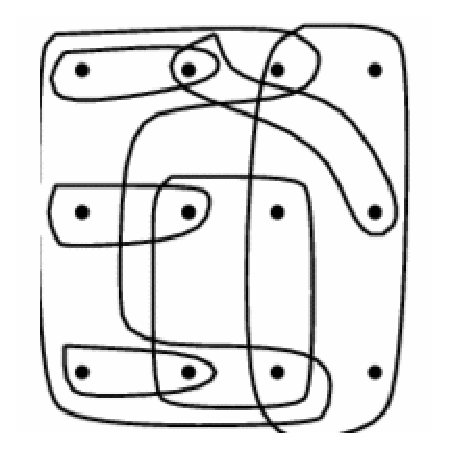
\includegraphics[width=0.6\textwidth]{02-background_and_motivation/img/set_cover_in}

(a)%
\end{minipage}\hfill{}%
\begin{minipage}[c]{0.45\textwidth}%
\centering

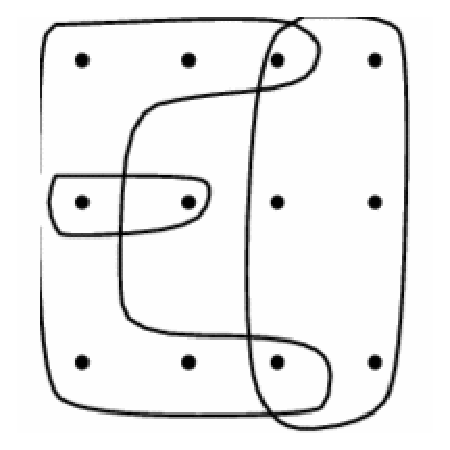
\includegraphics[width=0.6\textwidth]{02-background_and_motivation/img/set_cover_out}

(b)%
\end{minipage}\caption{The minimum set covering problem: (a) the problem input and (b) the
solution.\label{fig:The-minimum-set}}
\end{figure}


A different formulation considers the site selection problem as a
$p$-median problem, in which base station location is the only decision
variable considered. To each of the candidates solutions, an installation
cost is also associated. The $p$-median problem constitutes seeking
$p$ different locations each time, regardless of how distant the
sites are. The problem is to select one candidate site from each region
to install a base station such that the traffic capacity and the size
of the covered area are maximized with the lowest installation cost.


\subsection{Proposed solutions}

Aydin et al. \cite{Aydin:Heuristic.Optimization.Of.WCDMA} propose
a solution to the $p$-median problem based on three meta-heuristic
algorithms; a genetic algorithm, simulated annealing, and tabu search.
Their experimental study focuses on performance comparison between
the three algorithms.

A solution to the set covering problem is proposed by Hao et al. \cite{minimum.set.covering.problem:1997}.
A simulated annealing implementation was developed to solve the formulated
combinatorial problem. The results presented demonstrate the feasibility
of the proposed approach. Tutschku \cite{minimum.set.covering.problem:1998}
presents a specialized greedy algorithm to solve the same problem.
This work is part of the implementation of a planning tool prototype.
Mathar and Niessen \cite{minimum.set.covering.problem:2000} propose
a solution based on integer linear programming, which they claim finds
optimal solutions in most cases. They also introduce simulated annealing
as an approximate optimization technique. This approach substitutes
linear programming whenever an exact solution is out of reach because
of the complexity of the problem.

Amaldi et al. \cite{amaldi:planning.umts.base.station.location} offer
a discussion about the computational results of two different heuristics:
greedy search and tabu search. The problem formulation is based on
a set of candidate sites where the base stations can be installed,
an estimation of the traffic distribution and a propagation description
of the area to be covered. Some years later, the same authors \cite{Amaldi:Radio.planning.and.coveraga.optimization}
extended the problem formulation by also considering base station
configuration and hardware characteristics. In both works, they propose
a mixed integer programming model with which they aim to maximize
the trade-off between total traffic covered and total installation
costs. The only difference between the models is the constraint definition
of the linear program, where the constraints in \cite{amaldi:planning.umts.base.station.location}
are a subset of the constraints in \cite{Amaldi:Radio.planning.and.coveraga.optimization}.

Finally, Whitaker et al. \cite{GA.for.antenna.placement:2005} focus
on providing the required service coverage at the lowest possible
financial cost. Their framework supports the use of any multiple objective
optimization algorithm which seeks to approximate a Pareto front.
The performance of four different algorithms is explored, namely SEAMO,
SPEA2, NSGA-II and PESA.


\section{Optimizing antenna parameters}

There are many antenna parameters that control the coverage and interference
in the network, since the antenna shapes the emitted energy. Two important
parameters are the azimuth angle and the elevation angle (or tilt)
of the antenna. The antenna azimuth (shown in Figure \ref{fig:Antenna-azimuth})
is the direction in which the main beam of the horizontal pattern
points \cite{WCDMAforUMTS_RadioAccessForThirdGenerationMobileCommunications}.
The antenna tilt (shown in Figure \ref{fig:Antenna-tilt}) is defined
as the angle of the main beam of the antenna relative to the horizontal
plane \cite{WCDMAforUMTS_RadioAccessForThirdGenerationMobileCommunications}.
Both of these parameters have a great influence on network quality,
although antenna tilt requires less effort to implement, since most
modern radio networks already support remote electrical tilt. The
adjustment of these two parameters optimize some important aspects
of the network, namely:
\begin{itemize}
\item path loss between the base station and the mobile phone, since less
power is required for a connection, hence more power is available
for traffic; and
\item interference between neighboring cells, which leads to an overall
capacity increase.
\end{itemize}
\begin{figure}[h]
\centering

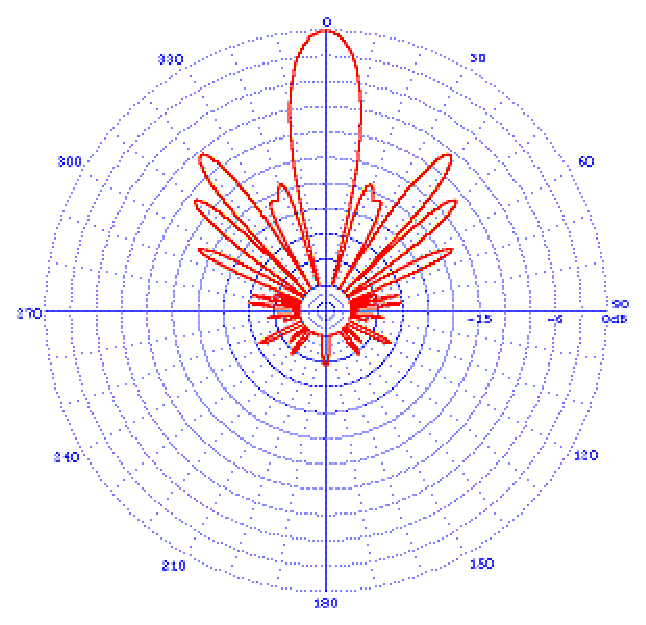
\includegraphics[width=0.3\textwidth]{02-background_and_motivation/img/azimuth}

\caption{A typical antenna azimuth pattern.\label{fig:Antenna-azimuth}}
\end{figure}


\begin{figure}
\centering

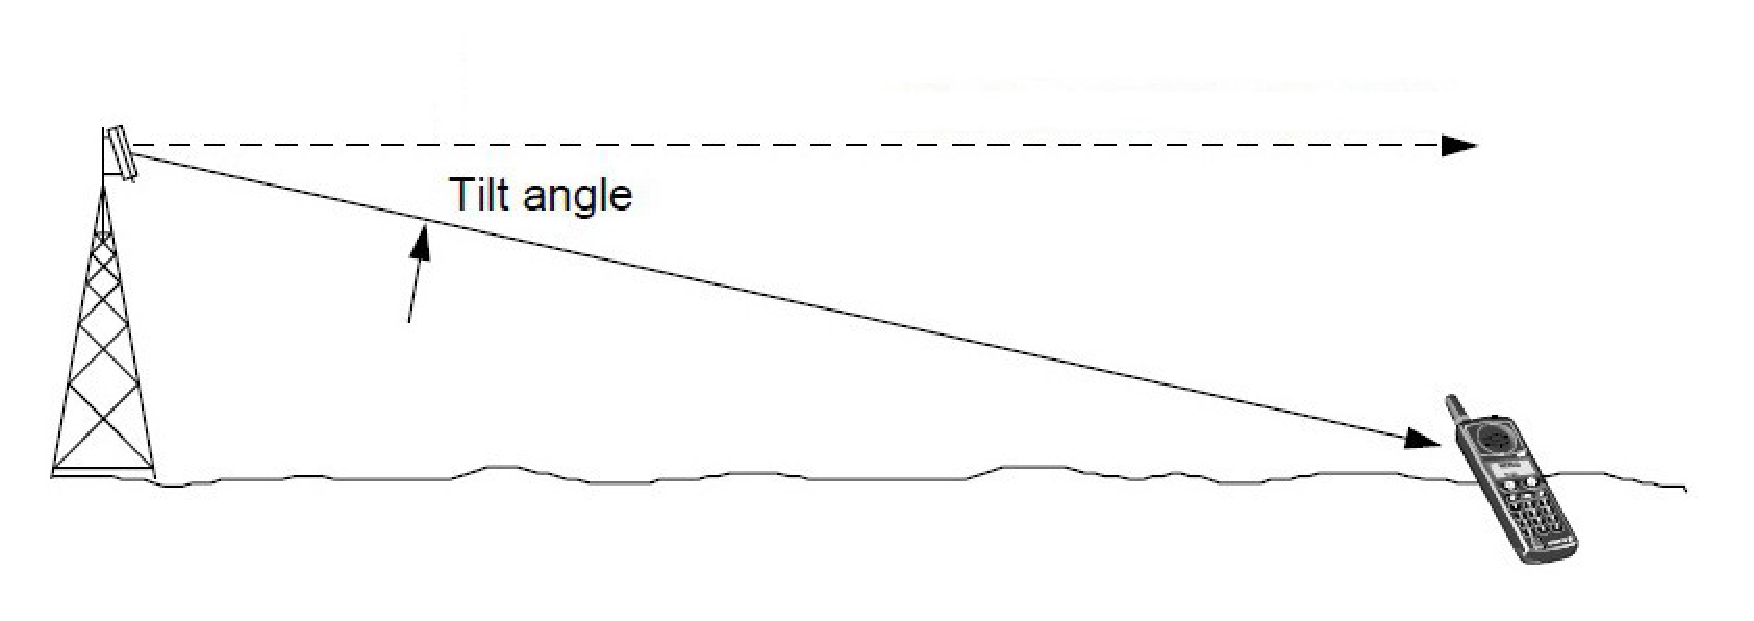
\includegraphics[width=0.6\textwidth]{02-background_and_motivation/img/tilt}

\caption{The antenna tilt angle with the horizontal plane.\label{fig:Antenna-tilt}}
\end{figure}



\subsection{Proposed solutions}

Karner \cite{MSc.antenna.optimization:2003} proposes an ``ad-hoc''
strategy for adjusting antenna azimuth and downtilt by analyzing the
structure of the network. The objective of this optimization is to
improve the results presented in \cite{Antenna.tilt.and.CPICH:2003}
by increasing the number of served users in the target area. In a
similar line of work, Jakl \cite{Jakl:PhD} included in his doctoral
thesis an antenna azimuth optimization algorithm, based on attempts
of avoiding coverage holes by properly adjusting the azimuth settings.

Siomina and Yuan \cite{Antenna.Configuration:2008} propose a framework
for automated optimization of antenna azimuth and tilt, including
both mechanical and electrical tilt. The implementation introduces
a simulated annealing algorithm that searches the solution space of
possible antenna configurations. The goal of the optimization is targeted
to address power sharing among cell channels and ultimately improve
High-Speed Downlink Packet Access (HSDPA) \cite{wiki:hsdpa} throughput.

Zhang et al. \cite{Antenna.azimuth.tilt:2009} present a method which
is composed of two optimization loops: the inner one and the outer
one. The inner loop concentrates on frequency planning while the outer
loop focuses on finding the optimal setting of antenna azimuth and
tilt for the current solution delivered by the inner loop. Although
frequency planning is not directly related to 3G network optimization,
we found this approach interesting enough to make a reference to it.
The inner loop could be easily replaced with some other optimization
target, e.g. common pilot channel power setting.


\section{Optimizing common pilot channel power}

The Common Pilot Channel (CPICH) is used as reference for handover
\cite{umts_world:handover}, cell selection \cite{3glteinfo:cellSelection},
and cell reselection \cite{flore2005:cell_reselection}. Whenever
a mobile phone is switched on, it tries to register with the cell
providing the highest received CPICH level. It also defines the effective
coverage area of the cell: according to the the CPICH power level,
the cell coverage area will enlarge or shrink. Consequently, by appropriately
adjusting the CPICH power at the base stations, the number of served
users per cell can be balanced among neighboring cells. This procedure
is called load balancing and it reduces interference, stabilizes network
operation, and facilitates radio resource management \cite{WCDMAforUMTS_RadioAccessForThirdGenerationMobileCommunications}.


\subsection{Proposed solutions}

Chen and Yuan \cite{CPICH.optimization:2008} optimize CPICH transmit
power starting from a uniform allocation (i.e. all cells are set with
the same transmit power level). Their objective is to enhance HSDPA
performance at cell edges while preserving control of R99 soft handover
\cite{wiki:soft_handover}. The solution approach is based on a linear-integer
mathematical model. A very similar problem and proposed solution is
presented by Siomina and Yuan \cite{CPICH.optimization:2007}. The
problem definition slightly differs from \cite{CPICH.optimization:2008}
as there is no reference to soft handover control. The solution is
also implemented as a linear program.

Olmos et al. \cite{CPICH.optimization:2003} apply simulated annealing
to the optimization of CPICH transmit powers in order to force mobile
phones to transmit to the best available cell in a service area. Their
results show decreased cell load with a consequently increased network
capacity.

Chen and Yuan \cite{CPICH.optimization:2009} present a two-phase
optimization algorithm for large-scale mobile networks. The algorithm
uses the total CPICH power consumption as a minimization objective.
The authors claim that the tabu-search-based algorithm can compute
near optimal solutions within a few seconds, even for large networks.


\section{Optimizing CPICH and antenna parameters}

Both the antenna tilt and azimuth directly affect the direction and
range in which the cell broadcasts its CPICH. Consequently, optimal
CPICH power is highly dependent on how the antenna tilt and azimuth
are configured at base stations. Ideal configuration of antenna tilt
and azimuth network-wise, with the objective of optimizing the CPICH
power consumption, is a challenging task. For this reason, many authors
have considered optimization methods that address all three parameters.


\subsection{Proposed solutions}

Varbrand et al. \cite{Coverage.optimization.on.CPICH.tilt.and.azimuth:2006}
approach the optimization of service coverage (see section \ref{sec:Optimizing-coverage})
by considering all three configuration parameters, namely: CPICH transmit
power, antenna tilt, and antenna azimuth. Their simulated annealing
algorithm searches the solution space of possible configurations in
order to find improvements in network performance and total transmitted
power. Interestingly, the algorithm is efficient enough to optimize
large networks without using excessive computing resources.

Siomina \cite{CPICH.and.antenna.tilt.optimization:2005} combines
optimization of base station antenna tilts and CPICH power to reduce
the total interference level and to improve network capacity. The
introduced algorithm optimizes the antenna downtilt setting so that
the total CPICH power in the network is minimized.

Neubauer et al. \cite{Antenna.tilt.and.CPICH:2003} present two optimization
algorithms for finding an optimal setting of antenna tilt and CPICH
power of the base stations. The first algorithm builds on a rule-based
approach, while the second one extends it by incorporating simulated
annealing. An evaluation of both techniques shows that the second
algorithm returns better results.

Jakl et al. \cite{GA.for.tilt.and.CPICH:2004} proposed a problem-specific
genetic algorithm to tackle the optimization of antenna tilts and
CPICH transmit powers. The goal of the optimization is to increase
network capacity. The implementation involves a deterministic fitness
selection scheme, a problem specific recombination operator and an
improved mutation operator. After the initial identification of the
best individuals, a local optimization technique is used to improve
their fitness.


\section{Optimizing coverage \label{sec:Optimizing-coverage}}

Coverage is maybe the most common optimization objective considered
in 3G network optimization. The objective function for coverage optimization
may be defined as follows:

\[
f_{cov}=\frac{A_{covered}}{A_{total}}
\]


where $A_{covered}$ represents the area covered by the network and
$A_{total}$ represents the total area under optimization. Thus, the
expression $f_{cov}$ represents the portion of the total area that
is actually under network coverage. This value ranges from 0 (no coverage)
to 1 (total coverage).

The area being optimized is usually divided in squares (or pixels)
of a certain size, which may vary from 10 to 100 meters, creating
a grid of a certain resolution. A square is considered covered, if
the signal to noise ratio is above a given threshold \cite{3GPP_TS_25.133}.
It is also common to use a test function $cov(x,y)$, which returns
1 if the square located at $(x,y)$ is covered, and 0 otherwise.


\subsection{Proposed solutions}

Siomina and Yuan \cite{Siomina:Minimum.pilot.power.for.service.coverage}
consider the problem of minimizing pilot power subject to the coverage
constraint. Their approach consists of mathematical programming models
and methods, based on a linear-integer mathematical formulation of
the problem. A special numerical analysis studies the trade-off between
service coverage and pilot power consumption for different test networks.

Capone et al. \cite{Amaldi:Radio.planning.and.coveraga.optimization}
investigate mathematical programming models for supporting decisions
on where to install new base stations and how to select their configuration
(antenna height and tilt, sector orientations, maximum emission power,
pilot signal, etc.) so to find a trade-off between maximizing coverage
and minimizing costs. The overall model takes into account signal-quality
constraints in both uplink and downlink directions, as well as the
power control mechanism and the CPICH signal.

Valkealahti et al. \cite{Coverage.balance:2002} propose a method
for automatic setting of CPICH power. The control algorithm applies
total transmission power measurements from the base station, neighboring
cells and mobile terminals to determine the pilot qualification. The
CPICH power is then periodically updated based on a group of heuristic
rules in order to improve coverage and load balance. A similar approach
is described by Parkinnen et al. \cite{Coverage.optimization.with.cost.function:2002}
where some network performance parameters are combined with service
coverage in a cost function. The pilot power of a cell is periodically
updated with a gradient descent method that minimizes the afore mentioned
function.


\section{Discussion}

In the field of 3G network optimization, comparing the efficiency
of different optimization methods has proven to be a very difficult
task. There are several reasons for this, among which we have identified
the following:
\begin{itemize}
\item The networks on which the experiments are carried out are not standardized.
Thus, it is problematic to set up an environment in which the presented
results may be reproduced.
\item There are no ``open'' implementations of 3G mobile network simulators.
On the contrary, there is a vast variety of proprietary (or ``closed'')
network simulators that only increase the ambiguity regarding the
experimental environment used for a certain network layout and configuration.
Moreover, some of the ``closed'' network simulators do not even
account on the built-in path loss estimation methods used.
\item Only a small part of the referenced optimization methods perform their
experiments on real-life networks, that have been already deployed
and are currently running. This fact creates a gap between the research
field and the industry (i.e. the application area) and it is counterproductive
for both the researchers and the network operators, since they don't
benefit from mutual collaboration.
\end{itemize}
We believe that the creation of a standardized framework would be
a great benefit in the field of 3G network optimization, as it would
allow researchers to compare different methods, results and solutions
in an easy, fast and objective manner. An effort in this direction
is the MOMENTUM project \cite{Momentum.project}. It was created with
the objective of setting up a standardized experimental environment
that would facilitate research cooperation and would ultimately benefit
from an improvement on the research field of 3G networks. The project
includes complete data about the terrain, properties of the service
area and hardware used in three different mobile networks. It offers
the researcher detailed information about real-life networks based
in Berlin, Lisbon and The Hague. As part of the package, there is
also a Java application programming interface (API) that eases the
implementation of some conventional tasks such as data parsing. The
main focus of project is on data, thus there is no network simulator
included. In any case, the researcher benefits from several included
traffic snapshots that help assessing different network configuration
settings. There have been no updates in the MOMENTUM project since
2005, when the last data corrections were introduced \cite{Momentum.project}.

In the context of this survey and after reviewing many different papers
on 3G network optimization, we can say that the MOMENTUM project has
not been widely adopted by the scientific community. Moreover, several
of the reviewed works do not offer detailed instructions on how to
resemble the experimental environment. Consequently, it is very complicated
(if not even impossible) to reproduce the presented results. Therefore,
the selection of optimization methods, based on the results presented
by their corresponding authors, is virtually meaningless, since the
results are not comparable with each other. For this reason, we have
decided to concentrate the following discussion on the optimization
methods used, leaving the results aside.


\subsection{The reproducibility problem}

A quick review of the state-of-the-art in 3G network optimization
indicates that software, providing good computational models, is a
very expensive tool for science. Moreover, since the vast majority
of this software is proprietary, it relies on closed source, formats
and protocols, which disclosure is explicitly forbidden by their licenses.
This fact creates a big hurdle to one of the key phases of scientific
methodology \cite{gauch2002scientific}: experimental reproducibility.


\subsection{Discussion about the presented methods}

Regarding the optimizations methods presented in previous chapters,
three distinctive groups emerge: genetic algorithms, linear programming
and other search methods.
\begin{description}
\item [{Genetic~algorithms}] These algorithms work on a population of
solutions that allows a more comprehensive search for optimal solutions.
As a direct consequence, an increase in running time is commonly observed.
The implementation effort of genetic algorithms is to some degree
higher than for simpler search methods (e.g. local search), but their
inherent structure greatly simplifies possible parallel implementations
and execution.
\item [{Linear~programming}] Linear optimization problems are widely used
in different optimization areas and there are many good software packages
to solve such problems. Consequently, if a problem can be modeled
as a continuous linear problem, there is usually no difficulty in
finding optimality. In the context of this survey, linear programming
has proven useful for coverage optimization in early network planning
stages.\\

\item [{Other~search~methods}] Other search methods%
\footnote{Namely, local search, simulated annealing and tabu search in the context
of this survey.%
} usually represent a compromise between running time and quality of
results. They rely on evaluating a great number of alternative configurations.
The number of parameters taken into account, as well as the evaluation
precision, directly influence their running time. These methods don't
excel in full simulation scenarios. On the other hand, some search
methods (e.g. tabu search) have powerful mechanisms to escape local
minima.
\end{description}
A short comparison of the optimization methods presented in this survey
is shown in Table \ref{tab:Comparison-of-optimization-methods}. The
comparison variables arise from the context in which the methods were
presented.

\begin{table}
\centering{\footnotesize \caption{A comparison among the presented optimization methods.\label{tab:Comparison-of-optimization-methods}}
}{\footnotesize \par}

{\footnotesize }%
\begin{tabular}{|c|c|c|}
\hline 
{\footnotesize Algorithm} & {\footnotesize Running time} & {\footnotesize Typical application}\tabularnewline
\hline 
\hline 
{\footnotesize Local search} & {\footnotesize Shorter} & {\footnotesize Solution quality improvement.}\tabularnewline
\hline 
{\footnotesize Tabu search} & {\footnotesize Shorter} & {\footnotesize Solution quality improvement.}\tabularnewline
\hline 
{\footnotesize Simulated annealing} & {\footnotesize Longer} & {\footnotesize Initial search of the solution space.}\tabularnewline
\hline 
{\footnotesize Genetic algorithm} & {\footnotesize Longer} & {\footnotesize Initial search of the solution space and solution quality
improvement.}\tabularnewline
\hline 
{\footnotesize Linear programming} & {\footnotesize (formulation dependent)} & {\footnotesize Coverage network planning.}\tabularnewline
\hline 
\end{tabular}
\end{table}



\section{Summary}

The variety of optimization problems that have been introduced in
the previous sections differ in many aspects like implementation,
running time and solution quality. Picking the right method for a
given situation depends on the optimization task and the desired results.
Since computation time is usually an important restriction, simpler
and faster methods may be preferable. 

Beside the convenience of a survey such as the one presented in this
work, it is very important to develop a feeling for the properties,
advantages and drawbacks of the respective methods. Moreover, radio
expert's recommendations regarding solution interpretation and feedback
from everyday network operation, are an essential input for creating
quality optimization methods. In this sense, and based on our own
experience, the expert's advice is irreplaceable and a most valuable
contribution to the research work.

Also, as it may be observed in some of the presented references, it
is often advisable to combine different methods. Therefore, a simple
optimization method may find a subset of reasonable parameter configuration,
whereas a more complex method could be applied afterward, to refine
the search. Sometimes it may also be useful to apply a simple search
method at the end to find better solutions in the vicinity of a current
promising one.
\cleardoublepage{}


\chapter{Framework design and implementation \label{chap:Framework-design-and-implementation}}

% First paragraph has no indentation.

\noindent There is a constant growing demand for hardware resources,
longer-processing times and more memory to follow the evolution of
3G radio networks \cite{maple2004parallel,crainic2006tackling,soldani2007autonomic}.
Fortunately, high-performance computer systems are increasingly accessible;
something made possible because of the emergence of computer clusters
and commodity hardware, capable of true parallel processing, e.g.
multi-core CPUs \cite{gorder2007multicore} and GPUs \cite{wen2011gpu}.
Moreover, the highly parallel structure present on GPUs makes them
more effective than CPUs for execution of algorithms where large blocks
of data need to be processed in parallel. Commodity GPUs have evolved
from being a graphic accelerator into a general-purpose processor.
They can achieve higher performance at lower power consumption and
lower costs when compared to conventional CPUs.

\vspace{3cm}


More than 20 years have passed since the world's first GSM mobile
call was made in Finland. Still, the coverage planning of the radio
network remains a key problem that all mobile operators have to deal
with. Moreover, it has proven to be a fundamental issue not only in
GSM networks, but also in modern standards such as the third generation
(3G) UMTS and the fourth generation (4G) LTE Advanced \cite{Saleh_On_the_coveraga_extension_in_LTE_networks:2010,Shabbir_Comparison_of_radio_propagation_models:2011,Siomina:Minimum.pilot.power.for.service.coverage,Valcarce_Applying.FDTD.to.the.coverage.prediction.of.WiMAX:2009}.
In radio networks is generally the case that the radio stations are
installed at fixed locations. For this reason, one of the primary
objectives of mobile-network planning is to efficiently use the allocated
frequency band to assure that the whole of the geographic area of
interest can be satisfactorily reached with the radio stations of
the network. To this end, radio-coverage prediction tools are of great
importance as it allows the network engineers to test different network
configurations before physically implementing the changes. Nevertheless,
radio-coverage prediction is a complex task due to the wide range
of various combinations of hardware and configuration parameters which
have to be analyzed in the context of different environments. The
complexity of the problem means that radio-coverage prediction can
be a computationally-intensive and time-consuming task, hence the
importance of fast and accurate prediction tools.

Although different mathematical models have been proposed for radio
propagation modeling, none of them excels in a network-wide scenario
\cite{Shabbir_Comparison_of_radio_propagation_models:2011}. A combination
of different models and parameters is generally needed in order to
calculate radio-propagation predictions for particular environments.
Moreover, since the number of deployed cells (transmitters) keeps
growing with the adoption of modern standards \cite{Saleh_On_the_coveraga_extension_in_LTE_networks:2010},
there is a clear need for a radio propagation tool that is able to
cope with larger work loads in a feasible amount of time.

Despite various options of commercial tools specialized in radio-propagation
modeling, the common thread among them is the restricted nature of
its usage, mostly dominated by black-box implementations. This fact
induces lack of adaptability, sometimes even combined with cumbersome
user interfaces that are not suitable for big batch jobs, involving
thousands of transmitters. Moreover, the evolution of any commercial
tool is strictly bounded to its vendor, forcing the user to adapt
its work-flow to it, when the opposite situation should be preferred.

To tackle the afore-mentioned issues, we present a high-performance
parallel radio-prediction tool for the open source Geographic Resources
Analysis Support System (GRASS). For its design, we have focused on
scalability, clean design and open nature of the tool, inspired by
the GRASS geographic information system (GIS). These facts make it
an ideal candidate for calculating radio-predictions of big problem
instances, i.e. real mobile networks containing thousands of transmitters.
This is also true for the scientific research community, since our
design may be used as a template for parallelization of computationally-expensive
tasks within the GRASS environment.


\subsection{Parallel computation on computer clusters}

In consideration of the high computational-intensity of predicting
the radio-coverage of a real mobile network, the use of a computer
cluster is required, i.e. a group of interconnected computers that
work together as a single system. To reach high levels of parallel
performance and scalability, this work discusses in detail the key
steps of parallel decomposition of the radio-coverage prediction problem
for real networks and the distribution of the computational load among
the computing nodes that belong to the cluster.

Such computer clusters typically consist of several commodity PCs
connected through a high-speed local network with a distributed file
system, like NFS \cite{Shepler_Network_file_system:2003}. One such
system is the DEGIMA cluster \cite{Hamada_Cluster_of_GPUs:2010} at
the Nagasaki Advanced Computing Center of the Nagasaki University.
This system ranked in the TOP 500 list of supercomputers until June
2012%
\footnote{http://www.top500.org%
}, and in June 2011 held the third place of the Green 500 list%
\footnote{http://www.green500.org%
} as one of the most energy-efficient supercomputers in the world.




\subsection{Objectives\label{sub:Objectives}}

The main goal of this work is to develop a radio prediction tool to
be used in large real-world network environments, such as the ones
currently deployed by several mobile operators around the world. To
achieve this, we have developed a high-performance parallel radio
prediction tool (PRATO) for radio networks. Therefore, our focus is
on the performance and scalability of PRATO, while other more dynamic
aspects of radio networks are not considered. Among these aspects
are code distributions, details of (soft) handover, and dynamics related
to radio resource management.



The performance evaluation of PRATO in a distributed computing environment
is a major objective of this work. Furthermore, by presenting a detailed
description of the design and implementation of the parallel version
of PRATO, we intend to provide guidelines on how to achieve high efficiency
levels of task parallelization in GRASS GIS. Additionally, we introduce
techniques to overcome several obstacles encountered during our research
as well as in related work, which significantly improve the quality
and performance of the presented implementation, e.g. the inability
to use GRASS in a threaded environment, lowering overhead of I/O operations,
saving simulation results asynchronously and independently from GRASS,
and improving load balancing with a new message-passing technique.



The paper is organized as follows. Section \ref{sec:Description-of-the-radio-coverage-prediction-tool}
gives a description of the radio prediction tool, including the propagation
model and GRASS GIS. Section \ref{sec:Design-and-implementation}
concentrates on the design principles and implementation details of
the radio propagation tool, for the serial and parallel versions.
Section \ref{sec:Simulations} discusses the experimental results
and their analysis. Finally, Section \ref{sec:Related-work} gives
an overview of relevant publications, describing how they relate to
our work, before drawing some conclusions.


\section{Description of the radio coverage prediction tool \label{sec:Description-of-the-radio-coverage-prediction-tool}}

PRATO is a high-performance radio-prediction tool for GSM (2G), UMTS
(3G) and LTE (4G) radio networks. It is implemented as a module for
the GRASS Geographical Information System (for details of GRASS see
Section \ref{sub:GRASS-GIS}). It can be used for planning the different
phases of a new radio-network installation, as well as a support tool
for maintenance activities related to network troubleshooting or upgrading. 

As a reference implementation, we have used the publicly available
radio coverage prediction tool, developed by Hrovat et al. \cite{Ozimek_Open.source.radio.coverage.prediction:2010}.
The authors of this work have developed a modular radio coverage tool
that performs separate calculations for radio-signal path loss and
antenna radiation patterns, also taking into account different configuration
parameters, such as antenna tilting, azimuth and height. The output
result, saved as a raster map, is the maximum signal level over the
target area, in which each point represents the received signal from
the best serving cell (transmitter). This work implements some well-known
radio propagation models, e.g. Okumura-Hata and COST 231, the later
is explained in more detail in Section \ref{sub:COST-231-model}.
Regarding the accuracy of the predicted values, the authors report
comparable results to those of a state-of-the-art commercial tool.
Therefore, we use the implementation developed by \cite{Ozimek_Open.source.radio.coverage.prediction:2010}
as the reference implementation for PRATO. Furthermore, to ensure
that our implementation is completely compliant with the afore-mentioned
reference, we have designed a comparison test that consists of running
both the reference and PRATO with the same input parameters. The test
results from PRATO and the reference implementation are identical.


\subsection{Propagation modeling\label{sub:COST-231-model}}

The COST-231 Walfisch-Ikegami radio-propagation model was introduced
as an extension of the well-known COST Hata model \cite{Shabbir_Comparison_of_radio_propagation_models:2011,Sarkar_Survey_of_radio_propagation_models:2003},
designed for frequencies above 2000~MHz. The suitability of this
model comes from the fact that it distinguishes between line-of-sight
(LOS) and non-line-of-sight (NLOS) conditions. Equation (\ref{eq:cost231_LOS})
describes the path loss when there is LOS between the transmitter
and the receiver.
\begin{equation}
PL_{\textrm{LOS}}(d)=42.64+26\log(d)+20\log(F),\label{eq:cost231_LOS}
\end{equation}
where $d$ is the distance (in kilometers) from the transmitter to
the receiver point, and $F$ is the frequency, expressed in MHz.

On the other hand, in NLOS conditions, the path loss is calculated
as

\begin{equation}
PL_{\textrm{NLOS}}(d)=L_{0}+L_{\textrm{RTS}}+L_{\textrm{MSD}},\label{eq:cost231_NLOS}
\end{equation}
where $L_{0}$ is the attenuation in free space, $L_{\textrm{RTS}}$
represents the diffraction from roof top to street, and $L_{\textrm{MSD}}$
represents the diffraction loss due to multiple obstacles.

In this work, as well as in the reference implementation \cite{Ozimek_Open.source.radio.coverage.prediction:2010},
the terrain profile is used for LOS determination. The wave-guide
effect in streets of big cities is not taken into account, because
the building data is not available. In order to compensate the missing
data, we include a correction factor, based on the land usage (clutter
data). This technique is also adopted by other propagation models
for radio networks, like the artificial neural networks macro-cell
model developed by Neskovic et al. \cite{Neskovic_Microcell_electric_field_strength_prediction_model:2010}.
Consequently, both Equations (\ref{eq:cost231_LOS}) and (\ref{eq:cost231_NLOS})
have an extra term for signal loss due to clutter ($L_{\textrm{CLUT}}$),
thus redefining the LOS and NLOS path losses as

\begin{equation}
PL_{\textrm{LOS}}(d)=42.64+26\log(d)+20\log(F)+L_{\textrm{CLUT}}\label{eq:cost231_LOS-1}
\end{equation}
and

\begin{equation}
PL_{\textrm{NLOS}}(d)=L_{0}+L_{\textrm{RTS}}+L_{\textrm{MSD}}+L_{\textrm{CLUT}}.\label{eq:cost231_NLOS-1}
\end{equation}



\subsection{GRASS Geographical Information System\label{sub:GRASS-GIS}}

As the software environment for PRATO we have chosen GRASS (Geographic
Resources Analysis Support System) \cite{neteler2002:GRASS_GIS},
which is a free and open-source software project that implements a
Geographical Information System (GIS). This GIS software was originally
developed at the US Army Construction Engineering Research Laboratories
and is a full-featured system with a wide range of analytical, data-management,
and visualization capabilities. Currently, the development of GRASS
GIS is supported by a growing community of volunteer developers.

The use of GRASS GIS as an environment for PRATO presents many advantages.
First, the current development of GRASS is primarily Linux-based.
Since the field of high performance computing is dominated by Linux
and UNIX systems, an environment with Linux support is critical for
this work. Software licensing is another important consideration for
choosing GRASS, since it is licensed under the GNU Public License
\cite{Stallman_GNU_License:1991} and imposes the availability of
the source code. This allows us to make potential modifications to
the system, thus adapting it for the parallel computation environment.
Moreover, being an open system, GRASS provided us with a great deal
of useful built-in functionality, capable of operating with raster
and vector topological data that can be stored in an internal format
or a relational database. For additional information about the GRASS,
we refer the reader to the numerous guides and tutorials available
online.


\section{Design and implementation \label{sec:Design-and-implementation}}

\begin{figure}
\centering

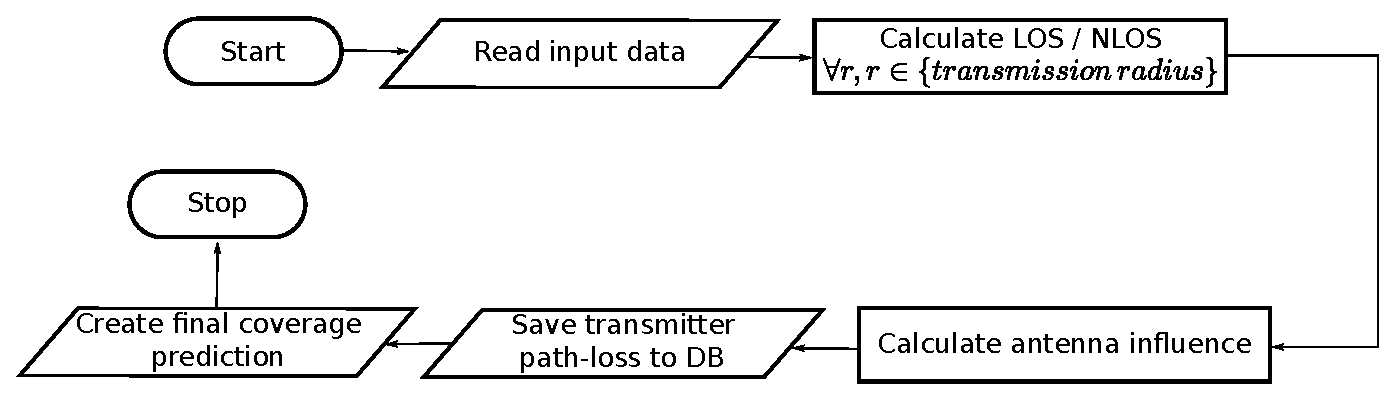
\includegraphics[width=0.67\columnwidth]{04-framework_design_and_implementation/img/serial_implementation_flow_diagram}

\caption{\textit{\emph{Flow diagram of the serial version.}}\textit{\label{fig:serial_version_flow_diagram}}}
\end{figure}


\begin{figure*}
\begin{minipage}[t]{0.49\textwidth}%
\centering

\includegraphics[width=0.8\columnwidth]{04-framework_design_and_implementation/img/isotrophic_calculation}

\caption{\textit{\emph{Example of raster map, showing the result of a path-loss
calculation from an isotropic source.\label{fig:path_loss-example}}}}
%
\end{minipage}\hfill{}%
\begin{minipage}[t]{0.49\textwidth}%
\centering

\includegraphics[width=0.8\columnwidth]{04-framework_design_and_implementation/img/antenna_calculation}

\caption{\textit{\emph{Example of raster map, showing the antenna influence
over the isotropic path-loss result.\label{fig:antenna-example}}}}
%
\end{minipage}
\end{figure*}



\subsection{Design of the serial version}

This section describes the different functions contained in the serial
version of PRATO, which is implemented as a GRASS module. Their connections
and data flow are depicted in \prettyref{fig:serial_version_flow_diagram},
where the parallelograms in the flow diagram represent input/output
(I/O) operations. 

Our design follows a similar internal organization as the radio planning
tool developed by Hrovat et al. \cite{Ozimek_Open.source.radio.coverage.prediction:2010},
but with some essential differences. Specifically, we have decided
to avoid the modular design to prevent the overhead of I/O operations
for communicating data between the components of the modular architecture.
Instead, we have chosen a monolithic design, in which all the steps
for generating the radio coverage prediction are calculated inside
one GRASS module. Regarding the way results are saved, our approach
employs a direct connection to an external database server, instead
of the slow built-in GRASS database drivers. To explicitly avoid tight
coupling with a specific database vendor, the generated output is
formatted in plain text, which is then forwarded to the database server.
Any further processing is achieved by issuing a query over the database
tables that contain the partial results for each of the processed
transmitters.


\subsubsection{Read input parameters\label{sub:Read-input-parameters}}

All input data are read in the first step (see ``Read input data''
in \prettyref{fig:serial_version_flow_diagram}), e.g. digital elevation
model, clutter data, transmitter configurations, and other service-dependent
settings. Their format differs based on the data they contain, namely:
\begin{itemize}
\item GRASS raster files are used for the digital elevation model and clutter
data, whereas
\item a text file is used for the transmitter configurations and other simulation-dependent
options.
\end{itemize}
Since the module accepts a considerable amount of input parameters,
they are read from a text-based initialization (INI) file. This is
far more practical than passing them as command-line parameters, which
would make them error-prune and difficult to read. Besides, the INI
file may contain configuration parameters for many transmitters. The
user selects which one(s) to use at run-time by passing a command-line
option.


\subsubsection{Isotropic path-loss calculation\label{sub:Path-loss-for-isotrophic-source}}

The first step here is to calculate which receiver points, $r$, are
within the specified transmission radius (see ``transmission radius''
in \prettyref{fig:serial_version_flow_diagram}). For these points,
the LOS and NLOS conditions are calculated, with respect to the transmitter
(see ``Calculate LOS/NLOS'' in \prettyref{fig:serial_version_flow_diagram}).
The following step consists of calculating the path loss for an isotropic
source (or omni antenna). This calculation is performed by applying
the COST-231 path-loss model, which was previously introduced in Section
\ref{sub:COST-231-model}, to each of the points within the transmission
radius around the transmitter. Depending on whether the receiver point
$r$ is in LOS or NLOS, either Equation~(\ref{eq:cost231_LOS-1})
or Equation~(\ref{eq:cost231_NLOS-1}) is respectively applied (see
``Apply COST-231, LOS'' or ``Apply COST-231, NLOS'' in \prettyref{fig:serial_version_flow_diagram}).

\prettyref{fig:path_loss-example} shows a portion of a raster map
with an example result of the isotropic path-loss calculation. The
color scale is given in dB, indicating the signal loss from the isotropic
source, located in the center. Also, the hilly terrain is clearly
distinguished due to LOS and NLOS conditions from the signal source.


\subsubsection{Antenna diagram influence\label{sub:Antenna-diagram-influence}}

This step considers the antenna radiation diagram of the current transmitter
and its influence over the isotropic path-loss calculation (see ``Calculate
antenna influence'' in \prettyref{fig:serial_version_flow_diagram}).
Working on the in-memory results generated by the previous step, the
radiation diagram of the antenna is taken into account, including
beam direction, electrical and mechanical tilt. \prettyref{fig:antenna-example}
shows a portion of a raster map, where this calculation step has been
applied to the results from \prettyref{fig:path_loss-example}. Notice
the distortion of the signal propagation that the antenna has introduced.


\subsubsection{Transmitter path-loss prediction\label{sub:Transmitter-path-loss-prediction}}

In this step, the coverage prediction of the transmitter is saved
in its own database table (see ``Save transmitter path-loss to DB''
in \prettyref{fig:serial_version_flow_diagram}), thus considerably
enhancing the write performance during the result-dumping phase, which
involves saving the path-loss results. This is accomplished by connecting
the standard output of the developed module with the standard input
of a database client. Naturally, the generated plain text should be
understood by the database server itself.


\subsubsection{Coverage prediction\label{sub:Final-coverage-prediction}}

The final radio coverage prediction, containing an aggregation of
the partial path-loss predictions of the involved transmitters, is
created in this step (see ``Create final coverage prediction'' in
\prettyref{fig:serial_version_flow_diagram}). The received signal
strength from each of the transmitters is calculated as the difference
between its transmit power and path loss for the receiver's corresponding
position. This is done for each point in the target area by executing
an SQL query over the tables containing the path-loss predictions
of each of the processed transmitters.

Finally, the output raster is generated, using the GRASS built-in
modules $v.in.ascii$ and $v.to.rast$, which create a raster map
using the results of the above-mentioned query as input. The raster
map contains the maximum received signal strength for each individual
point, as shown in \prettyref{fig:output_raster_example}. In this
case, the color scale is given in dBm, indicating the received signal
strength from the transmitters.

\begin{figure}
\centering

\includegraphics[width=0.95\columnwidth]{04-framework_design_and_implementation/img/final_coverage}

\caption{\textit{\emph{Example of raster map, displaying the final coverage
prediction of several transmitters. The color scale is given in dBm,
indicating the received signal strength.\label{fig:output_raster_example}}}}
\end{figure}



\subsection{Multi-paradigm parallel programming}

The implementation methodology adopted for PRATO follows a multi-paradigm
parallel programming approach in order to fully use the resources
of a computing cluster. To effectively use a shared memory multi-processor,
PRATO uses POSIX threads to implement parallelism \cite{Butenhof_Programming.with.POSIX.threads:1997}.
In a nutshell, POSIX thread is a POSIX standard for creating and manipulating
light-weight processes or threads. By using POSIX threads, multiple
threads can exist within the same process while sharing its resources.
For instance, an application using POSIX threads can execute multiple
threads in parallel by using the cores of a multi-core processor,
or use the system resources more effectively, thus avoiding process
execution-halt due to I/O latency by using one thread for computing
while a second thread waits for an I/O operation to complete. 

To use the computing resources of a distributed memory system, such
as a cluster of processors, PRATO uses the Message Passing Interface
(MPI) \cite{Gropp_Using_MPI:1999}. MPI is a message-passing standard
which defines syntax and semantics designed to function on a wide
variety of parallel computers. MPI enables multiple processes running
on different processors of a computer cluster to communicate with
each other. MPI was designed for high performance on both massively
parallel machines and on workstation clusters. It has been developed
by a broadly based committee of vendors, developers, and users.

In order to make the text more clear and to differentiate between
the programming paradigms used from here on, we will refer to a POSIX
thread simply as a `thread' and a MPI proccess as a `process'.


\subsection{Design of the parallel version\label{sub:Design-parallel}}

Keeping our focus on the performance of PRATO, we are introducing
a new distributed implementation to overcome computational-time constraints
that prevented the reference implementation from tackling big problem
instances \cite{Ozimek_Open.source.radio.coverage.prediction:2010}.

Some authors have already published their work on implementing parallel
versions of GRASS modules for solving different time-consuming tasks
\cite{Akhter_Porting_GRASS_raster_module_to_distributed_computing:2007,Campos_Parallel_modelling_in_GIS:2012,Sorokine_Parallel_visualization_in_GRASS:2007}.
However, one major drawback of GRASS as a parallelization environment
is that it is not thread-safe, meaning that concurrent changes to
a data set have undefined behavior. To overcome this problem, we present
a technique that saves the simulation results asynchronously and independently
from the GRASS environment, e.g. into an external database system.
This database system works also as an input source, serving data to
GRASS, whether it is used to aggregate the partial results of the
path-loss prediction or to visualize them. We also introduce a methodology
that allows the parallel implementation to be almost completely GRASS
independent. This means that a GRASS installation is needed on only
one of the nodes, i.e. the master node of the target computer cluster.
Also, a message-passing technique is proposed to distribute the work-load
among nodes hosting the worker processes. Using this technique, computing
nodes featuring more capable hardware receive more work than those
with weaker configurations, thus ensuring a better utilization of
the available computing resources despite hardware diversity.


\subsubsection{Master process\label{sub:Master-process}}

As it has been suggested before, the parallel version of PRATO follows
a master-worker model. The master process, for which the flow diagram
is given in \prettyref{fig:master_process}, is the only component
that should be run from within the GRASS environment. As soon as the
master process starts, the input parameters are read. This step corresponds
to ``Read input data'' in \prettyref{fig:master_process}, and it
is done in a similar way as in the serial version. In the next step,
the master process dynamically initiates the worker processes using
the available computing nodes (see ``Dynamic worker-process spawning''
in \prettyref{fig:master_process}), based on the amount of transmitters
for which the coverage prediction should be calculated. In other words,
this means that master process never starts more worker processes
than there are transmitters to be processed. However, most often is
the number of transmitters larger than the amount of available computing
nodes. Therefore, the master process can assign several transmitters
to each of the worker processes. For distributing the work among the
worker processes, the master process proceeds to decompose the loaded
raster data into arrays of basic-data-type elements, e.g. floats or
doubles, before dispatching them to the multiple worker processes
(see ``Input data broadcasting'' in \prettyref{fig:master_process}).
The decomposition of the data applies to the digital-elevation and
the clutter data only. In the next step, the master process starts
a message-driven processing loop (see ``Processing loop'' in \prettyref{fig:master_process}),
which main task is to assign and distribute the configuration data
of different transmitters among idle worker processes.

\begin{figure}
\centering

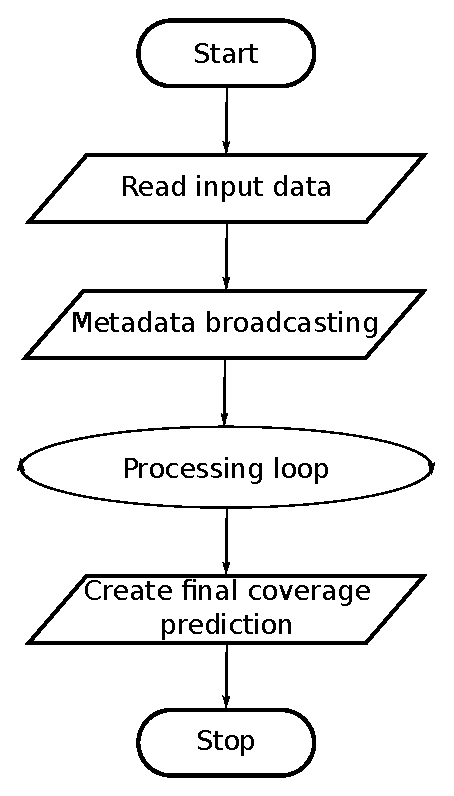
\includegraphics[width=0.4\columnwidth]{04-framework_design_and_implementation/img/master_process_flow_diagram}

\caption{\textit{\emph{Flow diagram of the master process.\label{fig:master_process}}}}
\end{figure}


The flow diagram shown in \prettyref{fig:processing_loop_in_master_process}
depicts in more detail the steps inside the ``Processing loop''
step of the master process. In the processing loop, the master process
starts by checking the available worker processes, which will calculate
the radio coverage prediction for the next transmitter. It is worth
pointing out that this step also serves as a stopping condition for
the processing loop itself (see ``Any worker still on?'' in \prettyref{fig:processing_loop_in_master_process}).
The active worker processes inform the master process they are ready
to compute by sending an idle message (see ``Wait for idle worker''
in \prettyref{fig:processing_loop_in_master_process}). The master
process then announces the idle worker process it is about to receive
new data for the next calculation, and it dispatches the complete
configuration of the transmitter to be processed (see ``Send keep-alive
message'' and ``Send transmitter data'' steps, respectively, in
\prettyref{fig:processing_loop_in_master_process}). This is only
done in case there are transmitters for which the coverage prediction
has yet to be calculated (see ``Any transmitters left?'' in \prettyref{fig:processing_loop_in_master_process}).
The processing loop of the master process continues to distribute
transmitter data among worker processes, which asynchronously become
idle as they finish the coverage-prediction calculations for the transmitters
they have been assigned by the master process. When there are no more
transmitters left, all the worker processes announcing they are idle
will receive a shutdown message from the master process, indicating
them to stop running (see ``Send stop message'' in \prettyref{fig:processing_loop_in_master_process}).
The master process will keep doing this until all worker processes
have finished (see ``Any worker still on?'' in \prettyref{fig:processing_loop_in_master_process}),
thus fulfilling the stopping condition of the processing loop.

\begin{figure}
\centering

\includegraphics[width=0.85\columnwidth]{04-framework_design_and_implementation/img/master_processing_loop_flow_diagram}

\caption{\textit{\emph{Flow diagram of the ``Processing loop'' step of the
master process.\label{fig:processing_loop_in_master_process}}}}
\end{figure}


Finally, the last step of the master process is devoted to creating
the final output of the calculation, e.g. a raster map (see ``Create
final coverage prediction'' in \prettyref{fig:master_process}).
The final coverage prediction of all transmitters is an aggregation
from the individual path-loss results created by each of the worker
processes during the ``Processing loop'' phase in \prettyref{fig:master_process},
which provides the source data for the final raster map. The aggregation
of the individual transmitter path-loss results is accomplished in
a similar way as in the serial version.


\subsubsection{Worker processes}

An essential characteristic of the worker processes is that they are
completely independent from GRASS, i.e. they do not have to run within
the GRASS environment nor use any of the GRASS libraries to work.
This aspect significantly simplifies the deployment phase to run PRATO
on a computer cluster, since no GRASS installation is needed on the
computing nodes hosting the worker processes.

The computations of the worker processes, for which the flow diagram
is given in \prettyref{fig:worker_process_flow_diagram}, are initialized
by data that are received from the master process at initialization
time (see ``Receive broadcasted data'' in \prettyref{fig:worker_process_flow_diagram}).
It is important to note that the received data contain the transmitter
and terrain-profile information which is common to all the coverage-prediction
calculations, therefore making each worker process capable of processing
any given transmitter.

The reason for the worker processes to be independent from GRASS arises
from the design of GRASS itself. Specifically, the existing GRASS
library, distributed with the GRASS GIS package, is not thread-safe,
because GRASS was designed as a system of small stand-alone modules
and not as a library for multi-threaded programs \cite{Blazek_GRASS_server:2004}.
Because of this limitation, it is not an option for a parallel implementation
to create separate threads for each worker process, since this would
mean worker processes should wait for each other to finish, before
accessing the target data. Consequently, the scalability of such implementation
would be very limited.

Because concurrent access to data within GRASS by multiple processes
yields undefined behavior, i.e. it is not thread-safe, the results
generated by the worker processes cannot be directly saved into the
GRASS data set. One possible solution would be to save the transmitter
path-loss prediction result through the master process, thus avoiding
concurrent access. However, sending intermediate results back to the
master process from the workers would represent a major bottleneck
for the scalability of the parallel version, since the results generated
by a parallel computation would have to be serially processed by the
master process alone. Instead, our approach allows each of the worker
processes to output its results into an external database server,
following an asynchronous and decoupled design. Each of the transmitter
path-loss prediction results are saved in separate tables, following
a similar design as the serial version. Moreover, worker processes
do this from an independent thread, which runs concurrently with the
calculation of the next transmitter received from the master process.
When compared to the serial version, the overlap between calculation
and communication achieved by the use of an auxiliary thread completely
hides the latency created by the result dumping task, and makes better
use of the system resources.

After the broadcasted data are received by all the worker processes,
each worker process proceeds to inform the master process that it
is ready (in an idle state) to receive the transmitter-configuration
data that defines which transmitter path-loss prediction to perform
(see ``Send idle message'' in \prettyref{fig:worker_process_flow_diagram}).
If the master process does not instruct to stop processing (see ``Has
stop message arrived?'' in \prettyref{fig:worker_process_flow_diagram}),
the worker process collects the transmitter configuration sent (see
``Receive transmitter data'' in \prettyref{fig:worker_process_flow_diagram}).
However, in case a stop message is received, the worker process will
wait for result-dumping threads to finish (see ``Wait for result-dump
threads'' in \prettyref{fig:worker_process_flow_diagram}) before
shutting down. The coverage calculation itself follows a similar design
as the serial version (see ``Coverage calculation'' in \prettyref{fig:worker_process_flow_diagram})
and it is executed for the received transmitter.

As it was mentioned before, the worker process launches an independent
thread to save the path-loss prediction of the target transmitter
to a database table (see ``Threaded save path-loss to DB'' in \prettyref{fig:worker_process_flow_diagram}).
It is important to note that there is no possibility of data inconsistency
due to the saving task being executed inside a thread, since path-loss
data from different workers belong to different transmitters and are
mutually exclusive. For this reason, there is no need for any concurrent
I/O overlapping \cite{Liao_Scalable_design_and_implementations_for_MPI_parallel_overlapping:2006}.

\begin{figure}
\centering

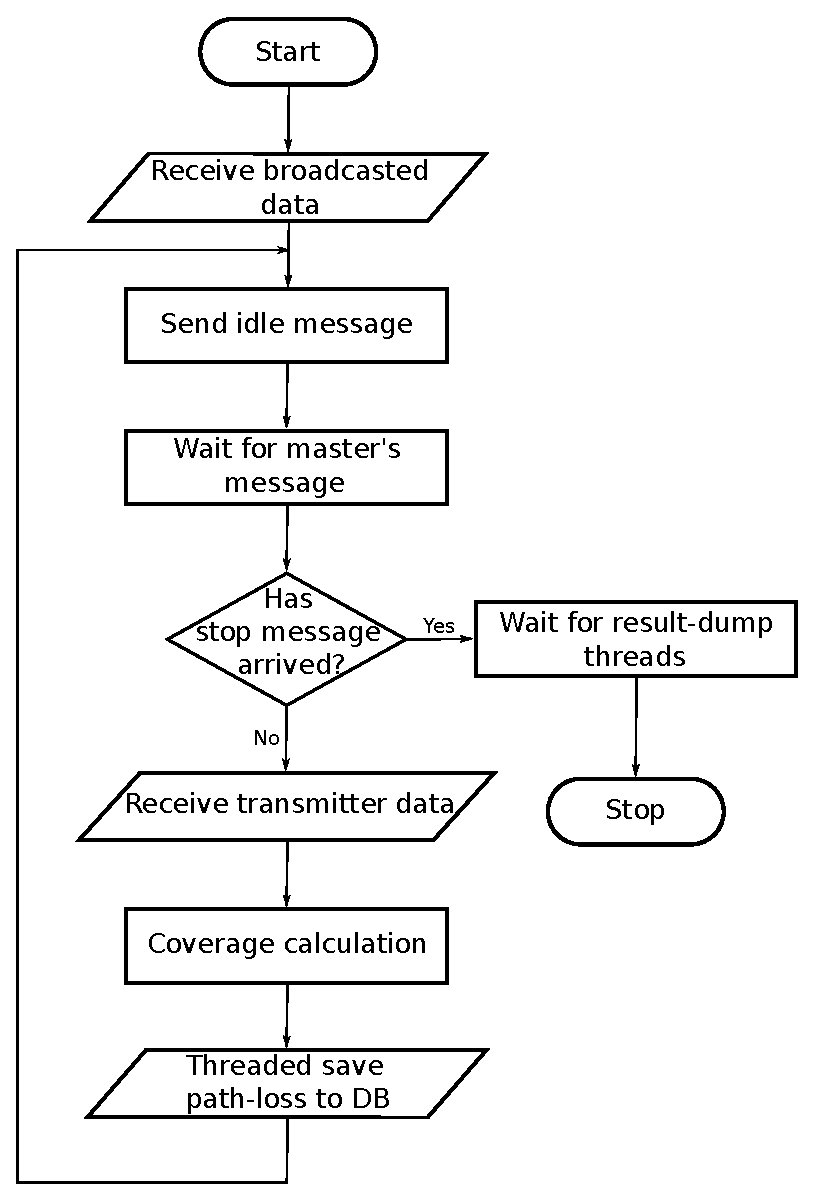
\includegraphics[width=0.7\columnwidth]{04-framework_design_and_implementation/img/worker_process_flow_diagram}

\caption{\textit{\emph{Flow diagram of a worker process.\label{fig:worker_process_flow_diagram}}}}
\end{figure}



\subsubsection{Master-worker communication\label{sub:Master-worker-communication}}

The selected message-passing technique introduced in this work might
seem too elaborated, but important reasons lay behind each of the
messages passed between master and worker processes. These decisions
are supported by the experimental results, introduced in Section~\ref{sec:Simulations}.

The first reason to implement the message-passing technique is to
support heterogeneous computing environments. In particular, our approach
focuses on taking full advantage of the hardware of each computing
node, thus explicitly avoiding the possible bottlenecks introduced
by the slowest computing node in the cluster. In other words, computing
nodes that deliver better performance get more calculations assigned
to the worker processes they host. The main advantages of this technique
are simplicity and negligible overhead, which contrast with more elaborated
approaches for parallel-task allocation in heterogenous clusters \cite{Bosque_A_parallel_computational_model_for_heterogenous_clusters:2006}.

A second reason for selecting a message-passing technique is related
to the flexibility for load balancing, which is of great importance
on heterogeneous cluster. This can be seen in \prettyref{fig:worker_process_flow_diagram}
where the master process, before delivering the transmitter-configuration
data, sends a message to the worker process indicating that it is
about to receive more work. This a priori meaningless message has
a key role in correctly supporting computer clusters. In general,
there are many different ways a parallel program can be executed,
because the steps from the different processes can be interleaved
in various ways and a process can make non-deterministic choices \cite{Siegel_Verification_of_halting_properties_for_MPI_programs:2007},
which may lead to situations such as race conditions \cite{Clemencon_MPI_Race_detection:1995}
and deadlocks. A deadlock occurs whenever two or more running processes
are waiting for each other to finish, and thus neither ever does.
To prevent the parallel version of PRATO from deadlocking, message
sending and receiving should be paired, being equal number of send
and receive messages on the master and worker sides \cite{Siegel_Verification_of_halting_properties_for_MPI_programs:2007}.

\prettyref{fig:master_worker_communication} depicts a diagram of
the master-worker message passing, from which the transmitter-data
transmission has been excluded for clarity. Note how each idle message
sent from the worker process is paired with an answer from the master
process, whether it is a keep-alive or a stop message.

\begin{figure}
\centering

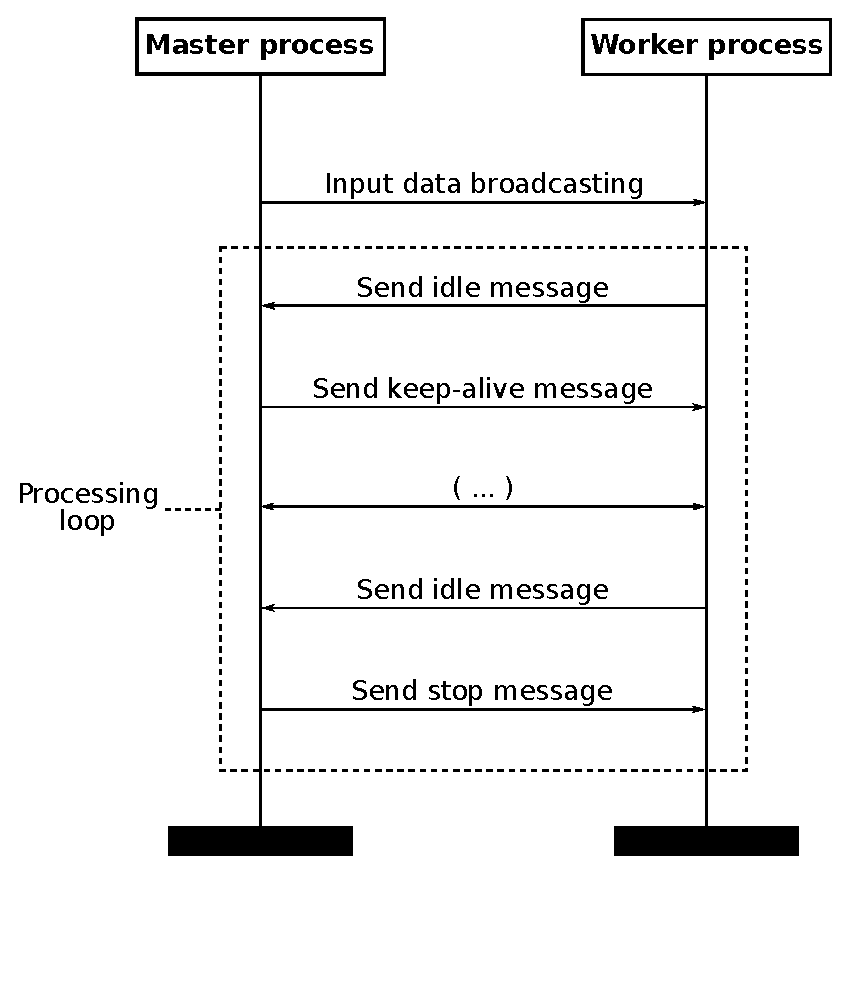
\includegraphics[width=0.85\columnwidth]{04-framework_design_and_implementation/img/master_worker_communication_diagram}

\caption{\textit{\emph{Communication diagram, showing message passing between
master and one worker process.\label{fig:master_worker_communication}}}}
\end{figure}



\section{Simulations \label{sec:Simulations}}

This section presents the simulations and analysis of the parallel
version of PRATO. Our aim is to provide an exhaustive analysis of
the performance and scalability of the parallel implementation in
order to determine if the objectives of this work are fulfilled. The
most common usage case for PRATO is to perform a radio-coverage prediction
for multiple transmitters, therefore, a straight forward parallel
decomposition is to divide a given problem instance by transmitter,
for which each coverage prediction is calculated by a separate worker
process.

The following simulations were carried out on 34 computing nodes of
the DEGIMA cluster. DEGIMA is a computer cluster located at the Nagasaki
Advanced Computing Center (NACC), in the University of Nagasaki, Japan.
The computing nodes are connected by a LAN, over a Gigabit Ethernet
interconnect, and share a NFS partition, from which all input and
intermediate files are accessed. 

Each computing node of DEGIMA features one of two possible configurations,
namely:
\begin{itemize}
\item Intel Core i5-2500T quad-core processor CPU, clocked at 2.30 GHz,
with 16 GB of RAM; and
\item Intel Core i7-2600K quad-core processor CPU, clocked at 3.40 GHz,
also with 16 GB of RAM.
\end{itemize}
During the simulation runs, the nodes equipped with the Intel i5 CPU
host the worker processes, whereas the master process and the PostgreSQL
database server (version 9.1.4) run each on a different computing
node, featuring an Intel i7 CPU. The database server is the only node
not writing or reading data from the common NFS partition. Instead,
all I/O is done on the local file system, which is mounted on a 8~GB
RAM disk.

All nodes are equipped with a Linux 64-bit operating system (Fedora
distribution). As the message passing implementation we use OpenMPI,
version 1.6.1, which has been manually compiled with the distribution-supplied
gcc compiler, version 4.4.4.


\subsection{Test networks}

To test the parallel performance of PRATO, we have prepared different
problem instances that emulate real radio networks of different sizes.
In order to create synthetic test data-sets with an arbitrary number
of transmitters we use the data of a group of 10 transmitters, which
we randomly replicate and distribute over the whole target area. The
configuration parameters of these 10 transmitters were taken from
the UMTS network deployed in Slovenia by Telekom Slovenije, d.d. The
path-loss predictions are calculated using the COST-231. The digital
elevation model has an area of 20,270~km$^{2}$, with a resolution
of 25~m$^{2}$, the same as the clutter data, which contains different
levels of signal loss based on the land usage. For all the points
within a transmission radius of 20~km around each transmitter, we
assume that the receiver is positioned 1.5~m above the ground, and
the frequency is set to 2040~MHz.


\subsection{Weak scalability}

This set of simulations is meant to analyze the scalability of the
parallel implementation in cases where the workload assigned to each
process (one MPI process per processor core) remains constant as we
increase the number of processor cores and the total size of the problem,
i.e. the number of transmitters deployed over the target area is directly
proportional to the number of processor cores and worker processes.
We do this by assigning a constant number of transmitters per core
while increasing the number of cores hosting the worker processes.
Consequently, we tackle larger radio-network instances as we increase
the number of cores. Here we test for the following numbers of transmitters
per worker/core: $\{5,10,20,40,80\}$, and increase the number of
workers per core from 1 to 128 in powers of 2.

Problems particularly well-suited for parallel computing exhibit computational
costs that are linearly dependent on the problem size. This property,
also referred to as algorithmic scalability, means that proportionally
increasing both the problem size and the number of cores results in
a roughly constant time to solution. Therefore, with this set of experiments,
we would like to investigate how well-suited the coverage-prediction
problem is for parallel computing environments.


\subsubsection{Results and discussion}

The results collected after the simulations for the weak-scalability
experiments are shown in Table \ref{tab:results_weak_scaling}. All
measurements express wall-clock times in seconds for each problem
instance, defined as number of transmitters per core (TX/core). Wall-clock
time represents real time that elapses from the start of the master
process to its end, including time that passes waiting for resources
to become available. They are plotted in \prettyref{fig:weak_scalability_time},
\textit{\emph{where the wall-clock time axis is expressed in base-10
logarithmic scale, whereas the axis representing the number of cores
is expressed in base-2 logarithmic scale.}}

\begin{table}
\caption{\textit{\emph{Wall-clock times (in seconds) of the simulation results
for weak scalability.\label{tab:results_weak_scaling}}}}


\centering

{\footnotesize }%
\begin{tabular}{ccccccccc}
\cmidrule{2-9} 
 & \multicolumn{8}{c}{{\footnotesize Number of cores}}\tabularnewline\addlinespace
\midrule 
{\footnotesize TX/core} & {\footnotesize 1} & {\footnotesize 2} & {\footnotesize 4} & {\footnotesize 8} & {\footnotesize 16} & {\footnotesize 32} & {\footnotesize 64} & {\footnotesize 128}\tabularnewline
\midrule
{\footnotesize 5} & {\footnotesize 92} & {\footnotesize 99} & {\footnotesize 118} & {\footnotesize 122} & {\footnotesize 123} & {\footnotesize 124} & {\footnotesize 125} & {\footnotesize 126}\tabularnewline
{\footnotesize 10} & {\footnotesize 140} & {\footnotesize 152} & {\footnotesize 171} & {\footnotesize 175} & {\footnotesize 177} & {\footnotesize 179} & {\footnotesize 180} & {\footnotesize 182}\tabularnewline
{\footnotesize 20} & {\footnotesize 244} & {\footnotesize 260} & {\footnotesize 278} & {\footnotesize 282} & {\footnotesize 284} & {\footnotesize 285} & {\footnotesize 287} & {\footnotesize 290}\tabularnewline
{\footnotesize 40} & {\footnotesize 451} & {\footnotesize 470} & {\footnotesize 491} & {\footnotesize 497} & {\footnotesize 500} & {\footnotesize 502} & {\footnotesize 504} & {\footnotesize 509}\tabularnewline
{\footnotesize 80} & {\footnotesize 865} & {\footnotesize 892} & {\footnotesize 920} & {\footnotesize 925} & {\footnotesize 928} & {\footnotesize 931} & {\footnotesize 937} & {\footnotesize 948}\tabularnewline
\bottomrule
\end{tabular}
\end{table}


\begin{figure}
\centering

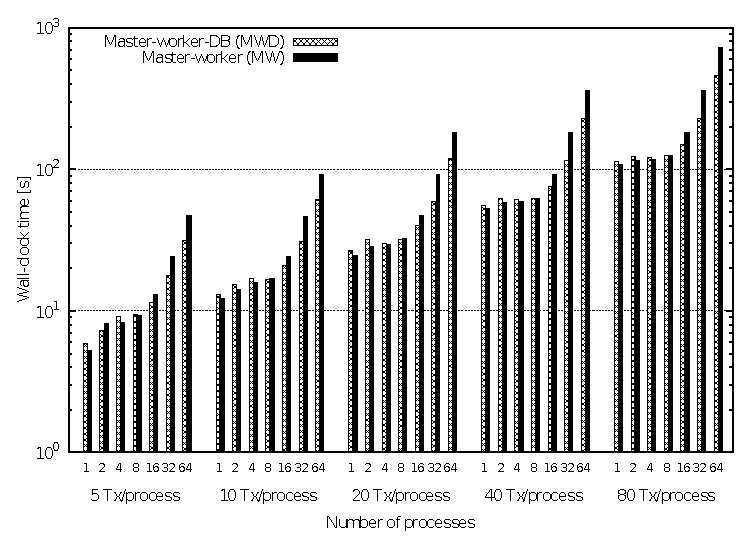
\includegraphics[width=1\columnwidth]{04-framework_design_and_implementation/img/weak_scaling-time_plot}

\caption{\textit{\emph{Measured wall-clock time for weak-scalability experiments
as shown in Table \ref{tab:results_weak_scaling}.}}\textit{ }\textit{\emph{Experiments
performed assigned one MPI worker process per available core. The
wall-clock time axis is expressed in base-10 logarithmic scale, whereas
the axis representing the number of cores is expressed in base-2 logarithmic
scale.\label{fig:weak_scalability_time}}}}
\end{figure}


The time measurements observed from the weak-scalability results show
that the wall-clock times do not grow rapidly, especially when the
number of cores is more than 8. Moreover, these times are almost constant
for bigger problem instances, revealing that the achieved level of
scalability gets close-to-linear as the amount of transmitters-per-core
increases. Certainly, the parallel version of PRATO scales especially
well when challenged with a big number of transmitters (10240 for
the biggest instance) over 128 cores. This fact shows PRATO would
be able to calculate the radio coverage prediction for real networks
in a feasible amount of time, since many operational radio networks
have already deployed a comparable number of transmitters, e.g. the
3G network within the Greater London Authority area, in the UK \cite{Number_of_base_stations_in_England}. 

Not being able to achieve perfect weak scalability is due to a number
of factors. Specifically, the overhead time of the serial sections
of the master process grow proportionally with the number of cores,
although the total contribution of this overhead remains low for large
problem sizes. Moreover, the communication overhead grows linearly
with the number of cores used.

To confirm these arguments, we analyze the times of each of the steps
taken by the master process relative to the total processing time.
To this end, we have created plots for three problem instances 5,
20 and 80 transmitters per core, which are shown in \prettyref{fig:weak_scaling-relative_times}.
The relative-processing-time plots follow the formula

\begin{equation}
RT=\frac{t_{\textrm{rd}}+t_{\textrm{ps}}+t_{\textrm{db}}+t_{\textrm{pl}}+t_{\textrm{cp}}}{t_{\textrm{total}}},\label{eq:relative_processing_time}
\end{equation}


\noindent where $t_{\textrm{rd}}$ is the ``Read input data'' wall-clock
time, $t_{\textrm{ps}}$ is the wall-clock time of the ``Dynamic
worker-process spawning'' step, $t_{\textrm{db}}$ is the wall-clock
time of the ``Input data broadcasting'' step, $t_{\textrm{pl}}$
is the wall-clock time of the ``Processing loop'' step, $t_{\textrm{cp}}$
is the wall-clock time of the ``Create final coverage prediction''
step, and $t_{\textrm{total}}$ is the total wall-clock processing
time. For a reference of the different steps taking part of the master
process, see \prettyref{fig:master_process}.

\begin{figure*}
\begin{minipage}[t]{0.31\textwidth}%
\centering

\includegraphics[width=1\columnwidth]{04-framework_design_and_implementation/img/weak_scaling_relative_time_plot_5}%
\end{minipage}\qquad{}%
\begin{minipage}[t]{0.31\textwidth}%
\centering

\includegraphics[width=1\columnwidth]{04-framework_design_and_implementation/img/weak_scaling_relative_time_plot_20}%
\end{minipage}\qquad{}%
\begin{minipage}[t]{0.31\textwidth}%
\centering

\includegraphics[width=1\columnwidth]{04-framework_design_and_implementation/img/weak_scaling_relative_time_plot_80}%
\end{minipage}

\caption{Relative times for the weak-scalability experiments.\emph{ }\textit{\emph{The
relative-processing time axes are expressed in linear scale, whereas
the axes representing the number of cores are expressed in base-2
logarithmic scale.\label{fig:weak_scaling-relative_times}}}}
\end{figure*}


From the relative-times plots, we see that, as we increase the number
of nodes, the largest fraction of the run-time is spent on the parallel
processing of transmitters, which scales notably well for larger problem
instances. The plotted relative times show that there is no dependency
between the relative processing times and the number of cores used,
confirming the good weak-scalability properties noted before. Additionally,
in all three plots we may observe a ``jump'' in the relative time
for the ``Input data broadcasting'' step that takes place when comparing
the result from 4 to 8 cores, i.e. from one to two computing nodes,
as each node hosts ``1 worker per core'' or a total of ``4 workers
per node''. This ``jump'' is due to the use of network communication
when more than one computing node participates in the parallel processing.
In addition, we may also conclude that the network infrastructure
has not been saturated with the data-passing load, since the relative
times for input-data broadcasting do not grow exponentially from 8
cores onward. Regarding the ``Create final coverage prediction''
step, we may see that as we increase the number of cores the relative
times grow proportionally for all three problem sizes.


\subsection{Strong scalability\label{sub:Strong-scalability}}

This set of simulations is meant to analyze the impact of increasing
the number of computing cores for a given problem size, i.e. the number
of transmitters deployed over the target area does not change, while
only the number of cores used is increased. Here we test for the following
number of transmitters: $\{64,128,256,512,1024,2048,4096\}$, and
increase the number of workers per core from 1 to 128 in powers of
2 for each problem size.


\subsubsection{Results and discussion}

The results of the time measurements collected after the simulations
for the strong-scalability experiments are shown in Table \ref{tab:results_strong_scaling}.
All times are expressed in seconds. These wall-clock time measurements
are plotted in \prettyref{fig:strong_scalability_time}, \textit{\emph{where
the time axis is expressed in base-10 logarithmic scale, whereas the
axis representing the number of cores is expressed in base-2 logarithmic
scale.}}

\begin{table}
\caption{\textit{\emph{Wall-clock times (in seconds) of the simulation results
for strong scalability.\label{tab:results_strong_scaling}}}}


\centering

{\footnotesize }%
\begin{tabular}{cccccccc}
\cmidrule{2-8} 
 & \multicolumn{7}{c}{{\footnotesize Number of transmitters}}\tabularnewline\addlinespace
\midrule 
{\footnotesize No. cores} & {\footnotesize 64} & {\footnotesize 128} & {\footnotesize 256} & {\footnotesize 512} & {\footnotesize 1024} & {\footnotesize 2048} & {\footnotesize 4096}\tabularnewline
\midrule
{\footnotesize 1} & {\footnotesize 714} & {\footnotesize 1392} & {\footnotesize 2740} & {\footnotesize 5437} & {\footnotesize 10830} & {\footnotesize 21562} & {\footnotesize 43217}\tabularnewline
{\footnotesize 2} & {\footnotesize 386} & {\footnotesize 734} & {\footnotesize 1419} & {\footnotesize 2791} & {\footnotesize 5535} & {\footnotesize 10996} & {\footnotesize 21987}\tabularnewline
{\footnotesize 4} & {\footnotesize 232} & {\footnotesize 408} & {\footnotesize 751} & {\footnotesize 1432} & {\footnotesize 2811} & {\footnotesize 5549} & {\footnotesize 11042}\tabularnewline
{\footnotesize 8} & {\footnotesize 155} & {\footnotesize 242} & {\footnotesize 409} & {\footnotesize 754} & {\footnotesize 1441} & {\footnotesize 2817} & {\footnotesize 5549}\tabularnewline
{\footnotesize 16} & {\footnotesize 113} & {\footnotesize 156} & {\footnotesize 244} & {\footnotesize 414} & {\footnotesize 759} & {\footnotesize 1447} & {\footnotesize 2821}\tabularnewline
{\footnotesize 32} & {\footnotesize 92} & {\footnotesize 114} & {\footnotesize 159} & {\footnotesize 245} & {\footnotesize 414} & {\footnotesize 760} & {\footnotesize 1449}\tabularnewline
{\footnotesize 64} & {\footnotesize 82} & {\footnotesize 94} & {\footnotesize 115} & {\footnotesize 159} & {\footnotesize 245} & {\footnotesize 420} & {\footnotesize 764}\tabularnewline
{\footnotesize 128} & {\footnotesize -} & {\footnotesize 83} & {\footnotesize 94} & {\footnotesize 116} & {\footnotesize 159} & {\footnotesize 248} & {\footnotesize 423}\tabularnewline
\bottomrule
\end{tabular}
\end{table}


\begin{figure}
\centering

\includegraphics[width=1\columnwidth]{04-framework_design_and_implementation/img/strong_scaling-time_plot}

\caption{\textit{\emph{Measured wall-clock time for strong-scalability experiments
as shown in Table \ref{tab:results_strong_scaling}. Experiments performed
assigned one MPI worker process per available core. The wall-clock
time axis is expressed in base-10 logarithmic scale, whereas the axis
representing the number of cores is expressed in base-2 logarithmic
scale.\label{fig:strong_scalability_time}}}}
\end{figure}


The time measurements show that small problem sizes per core have
a relatively large proportion of serial work and communication overhead.
Therefore, the performance deteriorates as the number of transmitters
per core approaches one. It can be observed in \prettyref{fig:strong_scalability_time}
that as we increase the number of transmitters used to solve a given
problem size, the slope of the curve generated by the progression
of wall-clock times tends to a flat line, i.e. as we increase the
number of transmitters there is no reduction in compute time. This
idea is more clearly noted in the test with smaller problem instances,
e.g. 64, 128 and 256 transmitters. In contrast, for the problems with
a number of transmitters larger than 512, the relative contribution
of the non-parallel steps to the wall-clock time is smaller, and a
larger portion of the time is spent on computing the transmitters
coverage in parallel (see Section \ref{sub:Design-parallel} for details
on the steps of PRATO algorithm). A more detailed discussion of the
reasons for the loss of parallel efficiency will be presented towards
the end of this section.

\begin{figure*}
\begin{minipage}[t]{0.45\textwidth}%
\centering

\includegraphics[width=1\columnwidth]{04-framework_design_and_implementation/img/strong_scaling-speedup_plot}

\caption{\textit{\emph{Measured speedup for strong-scalability experiments.}}\textit{
}\textit{\emph{The speedup axis is expressed in base-2 logarithmic
scale, whereas the axis representing the number of cores is expressed
in base-2 logarithmic scale.\label{fig:strong_scalability_speedup}}}}
%
\end{minipage}\hfill{}%
\begin{minipage}[t]{0.45\textwidth}%
\centering

\includegraphics[width=1\columnwidth]{04-framework_design_and_implementation/img/strong_scaling-efficiency_plot}

\caption{\textit{\emph{Measured parallel efficiency for strong-scalability
experiments.}}\textit{ }\textit{\emph{The parallel-efficiency axis
is expressed in linear scale, whereas the axis representing the number
of cores is expressed in base-2 logarithmic scale.\label{fig:strong_scalability_efficiency}}}}
%
\end{minipage}
\end{figure*}


In order to observe how well the application scales when compared
against a base case, we have also measured the performance of the
parallel implementation in terms of the speedup, which is defined
as

\begin{equation}
S(NP)=\frac{execution\, time\, for\, base\, case}{execution\, time\, for\, NP\, cores},\label{eq:speedup}
\end{equation}


\noindent where $NP$ is the number of cores executing the worker
processes. As the base case for comparisons we have chosen the parallel
implementation running on only one core and decided against using
the serial implementation. We consider that the serial implementation
is not a good base comparison for the parallel results as it does
not reuse resources between each transmitter coverage calculation
and it does not overlap I/O operations with transmitter computations.
In practice, this means that several concatenated runs of the serial
version would be considerably slower than the parallel but single
worker implementation, because the serial implementation is not able
to use all of the memory bandwidth and computing resources simultaneously.
Therefore such comparison would be entirely biased towards the parallel
implementation, showing super-linear scaling and speedups which would
not be real, as the parallel version is better equipped to make use
of the system resources by means of multiple threads.

Using the speedup metric, linear scaling is achieved when the obtained
speedup is equal to the total number of processors used. However,
it should be noted that perfect speedup is almost never achieved,
due to the existence of serial stages within an algorithm and communication
overheads of the parallel implementation \cite{Cruz_Particle.Flow.Simulation:2010}. 

\prettyref{fig:strong_scalability_speedup} shows the speedup of the
parallel implementation for up to 128 cores (running one worker process
per node), and compares seven different problem sizes with 64, 128,
256, 512, 1024, 2048 and 4096 transmitters deployed over the target
area. The number of transmitters used in these problem sizes are comparable
to several operational radio networks that have already been deployed
in England, e.g. Bedfordshire County with 69 UMTS base stations, Cheshire
County with 132 UMTS base stations, Hampshire County with 227 UMTS
base stations, West Midlands with 414 UMTS base stations, and Greater
London Authority with 1086 UMTS base stations \cite{Number_of_base_stations_in_England}.
Moreover, consider that it is common for a single UMTS base station
to host multiple transmitters. 

We can see that the significant reductions in wall-clock time for
large problem sizes shown in \prettyref{fig:strong_scalability_time}
are directly correlated with the speedup factors shown in \prettyref{fig:strong_scalability_speedup}.

\begin{figure*}
\begin{minipage}[t]{0.31\textwidth}%
\centering

\includegraphics[width=1\columnwidth]{04-framework_design_and_implementation/img/strong_scaling-relative_time_plot_256}%
\end{minipage}\qquad{}%
\begin{minipage}[t]{0.31\textwidth}%
\centering

\includegraphics[width=1\columnwidth]{04-framework_design_and_implementation/img/strong_scaling-relative_time_plot_1024}%
\end{minipage}\qquad{}%
\begin{minipage}[t]{0.31\textwidth}%
\centering

\includegraphics[width=1\columnwidth]{04-framework_design_and_implementation/img/strong_scaling-relative_time_plot_4096}%
\end{minipage}

\caption{Relative times for the strong-scalability experiments.\emph{ }\textit{\emph{The
relative-processing time axes are expressed in linear scale, whereas
the axes representing the number of cores are expressed in base-2
logarithmic scale.\label{fig:strong_scaling-relative_times}}}}
\end{figure*}


To study how well PRATO utilizes the available computing resources
we consider the parallel efficiency of the implementation, i.e. how
well the parallel implementation makes use of the available processor
cores. The definition of parallel efficiency is as follows:

\begin{equation}
E(NP)=\frac{S(NP)}{NP},
\end{equation}


\noindent where $S(NP)$ is the speedup as defined in Equation (\ref{eq:speedup}),
and $NP$ is the number of cores executing worker processes. \prettyref{fig:strong_scalability_efficiency}
shows the parallel efficiency of the parallel implementation for different
problem sizes as we increase the number of processing cores. 

The ideal case for a parallel application would be to utilize all
available resources, in which case the parallel efficiency would be
constantly equal to one as we increase the core count. From the plot
in \prettyref{fig:strong_scalability_efficiency}, we may observe
that the efficiency is less than one, hence the computational resources
are under utilized. In accordance to the previous analysis, the under
utilization of the computing resources is more significant for the
smaller problem sizes, where number of assigned transmitters per core
approaches one. This is due to the increased relative influence introduced
by serial and communication overheads, without which the parallel
implementation would not be feasible. On the other hand, the relative
time contribution of the serial and communication overheads is significantly
reduced as the work-load per core increases. Unsurprisingly, these
results confirm what it has previously been suggested during the weak-scaling
analysis, i.e. it is not worth parallelizing small problem instances
over a large number of nodes, since the time reduction due to computations
that make use of the extra parallel resources is surpassed by the
extra parallel initialization and communication overhead.

Similarly as in the weak-scaling test, we study the relative contribution
of each of the steps of the master process as we increase the number
of cores used for a fixed problem size. In this case, we have created
plots for three problem instances, namely 256, 1024 and 4096 transmitters,
which are shown in \prettyref{fig:strong_scaling-relative_times}.
The relative times shown are calculated using the formula depicted
in Equation (\ref{eq:relative_processing_time}).

We may observe the non-parallel steps comprising ``Read input data'',
``Dynamic worker-process spawning'', ``Input data broadcasting''
and ``Final coverage prediction'' contribute with a larger portion
of time as we increase the number of cores, because the total wall-clock
processing time decreases. Additionally, the low parallel efficiency
for small problem sizes, particularly for 256 transmitters (left-most
plot in \prettyref{fig:strong_scaling-relative_times}), is validated
as we see the relative small proportion of the radio-coverage calculation
(``Processing loop'') compared to the serial steps of the process.


\subsection{Load balancing}

In this section, we analyze the level of utilization of the computing
resources available at the computing nodes hosting the worker processes.
Computing-resource utilization is achieved by partitioning the computational
workload and data across all processors. Efficient workload distribution
strategies should be based on the processor speed, memory hierarchy
and communication network \cite{Clarke_Dynamic_load_balancing:2011}.

The parallel implementation of PRATO performs load-balancing using
point-to-point messages (see Section \ref{sub:Master-worker-communication})
between master and worker processes. When a worker process issues
an idle message (see ``Send idle message'' in \prettyref{fig:master_worker_communication}),
the worker process will block until the message arrives to the master
process. A similar situation occurs when the master process signals
a worker back, whether to indicate it to shutdown or to continue working.
Since the process-to-core mapping is one-to-one, blocking messages
typically waste processor cycles on a computing node \cite{Bhandarkar_Adaptive_load_balancing_for_MPI:2001}.
Specifically, we would like to verify the penalties that such synchronization
technique has on the scalability of the parallel implementation.

We evaluate the load empirically \cite{Watts_A_practical_approach_to_dynamic_load_balancing:1998}
by using the following metric as an indicator of the load balancing
among processes:

{\small 
\begin{equation}
LB(NP)=\frac{minimum\, execution\, time\, among\, NP\, cores}{processing\, loop\, time\, of\, master\, process},
\end{equation}
}{\small \par}

\noindent where $NP$ is the number of cores executing worker processes.
Taking the processing-loop time of the master process ensures we measure
the overhead of the message passing during the time while the coverage
prediction is being executed by the workers. This means that the time
measurement is performed excluding the serial parts of the process,
i.e. after the common data have been broadcasted to all worker processes
(``Input data broadcasting'' in \prettyref{fig:master_process}),
until the beginning of the last step (``Create final coverage prediction''
in \prettyref{fig:master_process}).

High performance is achieved when all cores complete their work within
the same time, hence showing a load-balancing factor of one. On the
other hand, lower values indicate disparity between the run times
of the various worker processes sharing the parallel task, thus reflecting
load imbalance.


\subsubsection{Results and discussion}

For this set of experiments, we have chosen the same problem sizes
as for strong scalability in Section \ref{sub:Strong-scalability},
where the coverage predictions are calculated up-to 128 cores, running
on 32 computing nodes.

\begin{figure}
\centering

\includegraphics[width=1\columnwidth]{04-framework_design_and_implementation/img/strong_scaling-load_balancing_plot}

\caption{\textit{\emph{Load balancing among worker processes.\label{fig:load_balancing}}}}
\end{figure}


From the plot shown in \prettyref{fig:load_balancing}, it is clear
that the influence of the message-passing overhead over the processing
time is inversely proportional to the amount of work each worker process
receives. Additionally, for the biggest problem instances (1024, 2048
and 4096 transmitters), parallel-process execution times are within
95\% of a perfect load-balancing factor, and within 90\% for problem
sizes with 256 and 512 transmitters, showing a very good performance
of the dynamic task assignment, driven by our message-passing technique.
For problem instances of 64 and 128 transmitters, the parallel-process
times are within 80\% of the perfect load balancing, showing that,
as the number of transmitters per core approaches to one, latencies
introduced by several hardware and OS-specific factors (e.g. TurboBoost,
process affinity, etc.) are influential over the total process time.
Particularly, message-passing is not able to compensate these latencies
as it is executed only once per worker process.

It is worth pointing out that the very good load-balancing factors
shown here are not only merit of the message-passing technique. The
result dumping of partial path-loss predictions, performed by the
worker processes in a separate thread into an external database server,
prevents data synchronization from occurring at each iteration of
the parallel process, consequently improving the load-balancing factors
significantly.


\section{Related work \label{sec:Related-work}}

As it has been mentioned before, the reference implementation for
PRATO is the work done by Hrovat et al. \cite{Ozimek_Open.source.radio.coverage.prediction:2010}.
The reported results show a comparable quality to those of a professional
radio-planning tool. Since the results of the conducted comparison
tests showed identical results between PRATO and this work, we may
conclude that PRATO reaches solutions of comparable quality to those
of a professional tool. However, a performance comparison with this
work has not been performed, because it only deals with serial implementations. 

A different example of a GIS-based open-source radio planning tool,
called Q-Rap, has been presented in \cite{QRap}. Developed by the
University of Pretoria and the Meraka Institute of South Africa, the
software was made publicly available in May 2010. Its design is geared
towards an end-user tool with a graphical user interface, not appropriate
for big batch jobs involving thousands of transmitters, or even parallel
job execution. It is implemented as a plug-in for the Quantum GIS
(QGIS) open source system \cite{QuantumGIS}.

The task-parallelization problem within the GRASS environment has
been addressed by several authors in different works. Campos et al.
\cite{Campos_Parallel_modelling_in_GIS:2012} present a collection
of GRASS modules for watershed analysis. Their work concentrates on
different ways of slicing raster maps to take advantage of a potential
MPI implementation, but there are no guidelines for work replication.
Moreover, the hardware specification, on which the experiments have
been run, is missing, making it very difficult to build upon this
work.

On the field of high-performance computing, Akhter et al. \cite{Akhter_Porting_GRASS_raster_module_to_distributed_computing:2007}
have presented implementation examples of a GRASS raster module, used
to process vegetation indexes for satellite images, for MPI and Ninf-G
environments. The main drawback with their methodology is the compulsory
use of GRASS libraries in all the computing nodes that take part in
the parallel calculation, making them more difficult to setup. Moreover,
the authors explicitly acknowledge a limitation in the performance
of their MPI implementation for big processing jobs. The restriction
appears due to the computing nodes being fixed to a specific range,
since the input data are equally distributed among worker processes,
creating an obstacle for load balancing in heterogeneous environments.
It is worth pointing out that in the parallel implementation of PRATO
we specifically address this problem with our message-passing technique.

Similarly, Huang et al. \cite{Huang_Cluster_based_parallel_GIS:2011}
use the parallel inverse distance weighting interpolation algorithm
as a parallel-pattern example. Although it is not explicitly noted,
it can be concluded that the computing nodes make use of the GRASS
environment, again making them more difficult to setup. Moreover,
since the amount of work is evenly distributed among all processes
(including the master one), their approach would also show decreased
efficiency in heterogeneous environments.


\section{Summary}

We have presented the design and implementation of PRATO, a parallel
radio-coverage prediction tool for GRASS GIS. Extensive simulations
were performed in the DEGIMA computer cluster of the Nagasaki Advanced
Computing Center. The results have been analyzed to determine the
level of scalability of the implementation, as well as the impact
of the introduced patterns for parallel algorithm design within GRASS
GIS.

The conducted analysis shows that PRATO is able to calculate the radio-coverage
prediction of real-world mobile networks in a reduced amount of time
with a high scalability level. The promising results also show the
great potential of our approach to parallelize other time-consuming
tasks for GRASS GIS, although this point still has to be fully demonstrated.
Particularly, the gathered results suggest that our approach would
be also beneficial in the area of mobile network optimization, where
thousands of simulations take part of the evaluation step during an
optimization process. Still, further research is needed on how this
method may be fully exploited.

Nevertheless, as PRATO is a free and open-source software project,
it can be readily modified and extended to support, for example, other
propagation models and post-processing algorithms. This characteristic
defines a clear advantage when compared to commercial and closed-source
tools.


\cleardoublepage{}


\chapter{Service-Coverage Optimization \label{chap:06-Experimental-evaluation-the-service-coverage-problem}}

% First paragraph has no indentation.

\noindent The high-performance of PRATO, the radio-coverage simulation
framework presented in Chapter~\ref{chap:04-Framework-design-and-implementation},
allows dealing with big problem instances in a reduced amount of time.
Additionally, it enables tackling optimization problems that, because
of their size, are out-of-reach of traditional approaches, mainly
due to the computational-time complexity of their objective-function
evaluation.

In this chapter, the challenge is to exploit PRATO for solving one
of the classic optimization problems of radio networks: the service-coverage
problem. Considering the minimization of the total amount of pilot
power subject to a full coverage constraint, a novel optimization
approach is introduced. The presented method, based on parallel autonomous
agents, gives very good solutions to the problem in an acceptable
amount of time. The parallel implementation takes full advantage of
GPU hardware in order to achieve considerable speedup. The analysis
of the experimental results, considering six real-world radio networks
of different sizes, studies solution-quality and performance aspects.

The content of this chapter extends the research work published by
the author in~\cite{Benedicic_Pilot.power.optimization:2010} and~\cite{Benedicic-A_GPU_based_parallel_agent_optimization_approach:2013}.
The rest of this chapter is organized as follows. Section~\ref{sec:06-Motivation}
gives a description of the coverage problem and its motivation from
the mobile operator's perspective. In Section~\ref{sec:06-Related-work},
a short overview of related research works is given, before introducing
the key elements of the service-coverage problem in Section~\ref{sec:06-Radio_network_model},
and formally defining it in Section~\ref{sec:06-Problem-definition}.
The parallel-agent approach, as well as the strategies used for result
comparison, are presented in Section~\ref{sec:06-Optimization-approaches},
followed by the simulations and their analyses in Section~\ref{sec:06-Simulations}.


\section{Motivation \label{sec:06-Motivation}}

Solving the service-coverage problem for radio networks has received
a great deal of attention in the past years. Its complexity demands
the confluence of different skills in areas such as propagation of
radio signals, telecommunications and information systems, among others.

Even several decades after the launch of the first commercial GSM
network, service-coverage planning remains a key problem that all
mobile operators have to deal with. Its intricacy arises from the
wide range of different combinations of configuration parameters and
their evaluation-time complexity.

Regardless of the mobile technology used, e.g., GSM, UMTS or LTE,
a lower transmit power generates less interference, which, in turn,
translates into more capacity of the radio link (see Chapter~\ref{chap:02-Principles_of_mobile_radio_networks}).
Additionally, reducing the transmit-power usage is also related to
issues regarding human exposure to the electromagnetic fields generated
by BS antennas~\cite{Esposito_Genetic.optimization.for.optimum.3G.network.planning:2010}.
During the past few years, public opinion has been extremely sensitive
regarding this issue, and many countries have already imposed safety
standards to limit the electromagnetic field levels produced by antennas
in a given range.

From the UMTS perspective, minimizing pilot-power usage leaves more
power available for increased network capacity. This is especially
important if the traffic and other channels are configured relative
to the pilot channel~\cite{WCDMAforUMTS_RadioAccessForThirdGenerationMobileCommunications}.
Moreover, as the demand for internet access and data services increases~\cite{Cunningham_Network.growth.theory.and.evidence:2010},
so does the pressure on existing network infrastructure, making parameter
optimization the only viable solution in the short-term~\cite{Nawrocki-Understanding_UMTS_radio_network_modelling_and_optimisation:2006}.

\bigskip{}


The idea of using autonomous agents for optimization is not new. It
has proven to be a solid optimization approach for solving different
types of problems, not only within the area of radio networks~\cite{Cheung_Realtime.video.using.agent.over.3G.networks:2005,Esposito_Genetic.optimization.for.optimum.3G.network.planning:2010},
but also in other fields~\cite{Valcarce_Applying.FDTD.to.the.coverage.prediction.of.WiMAX:2009,Vasile_Hybrid.multiagent.approach.for.optimization:2009}.
The increased computational-time complexity when dealing with big
problem instances is tackled using a parallel, agent-based algorithm
on GPU. This minimizes the overhead when deploying a larger number
of agents working in parallel over the service area, only limited
by the amount of memory available on the GPU.


\section{Related work \label{sec:06-Related-work}}

There are several approaches in the literature that address the service-coverage
problem in radio networks~\cite{Amaldi-Radio_planning_and_coverage_optimization_of_3G_networks:2008,Nawrocki-Understanding_UMTS_radio_network_modelling_and_optimisation:2006,Siomina_Pilot.power.optimization:2004}.
Some of them even claim to achieve near-optimal solutions~\cite{Siomina:Minimum.pilot.power.for.service.coverage}.
As a matter of fact, most formulations are only useful for small network
instances and often fail when challenged with larger, real-world networks.

A genetic-algorithm approach for solving the service-coverage problem
for GSM networks was presented in~\cite{Lieska-Radion_coverage_optimization_with_genetic_algorithms:1998}.
The proposed solution is based on the physical distribution of BSs
in order to maximize coverage. The simulations were performed on a
test network with 40 candidate sites for BS antennas.

In~\cite{Siomina:Minimum.pilot.power.for.service.coverage}, Siomina
and Yuan considered the problem of minimizing the total amount of
pilot power for UMTS networks, subject to a full coverage constraint.
They tackled the problem with an iterative linear-programming approach,
reporting very good results for some test networks, containing from
15 to 65 base stations. The authors noted that bigger problem instances
could not be solved because of hardware constraints on the target
platform.

As for LTE networks, the service-coverage problem was addressed in~\cite{Thampi-A_sparse_sampling_algorithm_for_self_optimization_of_coverage_in_LTE:2012}.
The authors presented an algorithm, based on reinforcement learning,
to tackle three aspects of the coverage problem, i.e., coverage holes,
weak coverage and pilot pollution. The experimental simulations, performed
on 3 BSs, used different antenna-tilt configurations as the proposed
solutions.

The service-coverage problem, as presented in this chapter, corresponds
to achieving full coverage of the target area, without coverage holes.


\section{Radio-network model \label{sec:06-Radio_network_model}}

Extending the representation of a radio-network model from~\cite{Nawrocki-Understanding_UMTS_radio_network_modelling_and_optimisation:2006},
this section presents the definitions of the elements included in
the mathematical model used for the simulations.

The goal here is to analyze the state of the network in a given situation,
i.e., a \textquoteleft{}snapshot\textquoteright{} at an arbitrary
instance. Radio-network planning tools, including the commercial ones,
typically rely on static analysis~\cite{Niemela-Performance_of_static_WCDMA_simulator:2005}.

A snapshot consists of a set of UEs having individual properties,
such as location and equipment type, that provides an estimate of
the average network behavior. The static approach inherently ignores
dynamic effects that influence the system, like fast power control,
but the analysis relies on having multiple independent snapshots to
produce an average behavior.

Another alternative is to consider using a dynamic tool for radio-network
planning~\cite{Hamalainen-Advanced_WCDMA_radio_network_simulator:1999,Hoppe-Fast_planning_of_efficient_WCDMA_radio_networks:2001}.
Dynamic simulation considers all Radio-Resource Management~(RRM\nomenclature[A]{RRM}{Radio-resource management})
functionality, as well as user mobility. However, when compared to
the static approach, a major disadvantage of the dynamic simulation
is the large computational time it requires. This clearly excludes
the possibility of achieving fast performance evaluations of a network,
which is one of the objectives of this thesis.

Considering that the performance of a static approach was demonstrated
to provide sufficiently accurate results compared to a fully dynamic
approach~\cite{RadioNetworkPlanningAndOptimisationForUMTS,Laiho-Verification_of_WCDMA_network_planning_prediction_with_dynamic_simulations:2001},
the former one is implemented in this work.

For additional information regarding mathematical models for radio
networks and signal propagation, see~\cite{RadioNetworkPlanningAndOptimisationForUMTS,Nawrocki-Understanding_UMTS_radio_network_modelling_and_optimisation:2006,Stuber-Principles_of_mobile_communication:2011}.


\subsection{Basic elements}

Consider a radio network with a set of antenna installations (cells),
$C$\nomenclature[S]{$C$}{Set of antenna installations (cells) in a mobile network}.
A RSG of a given resolution represents a geographical area, $A_{\mathrm{total}}$,
within which a set of UEs, $M$\nomenclature[S]{$M$}{Set of mobile devices or users of a mobile network},
is spatially distributed over the pixels of $A_{\mathrm{total}}$.
Further, $l_{cm}^{\downarrow}$\nomenclature[S]{$l_{cm}^{\downarrow}$}{Downlink attenuation factor between cell $c\in C$ and mobile $m\in M$}
is defined as the downlink attenuation factor between cell $c\in C$
and UE $m\in M$. Similarly, $l_{mc}^{\uparrow}$\nomenclature[S]{$l_{mc}^{\uparrow}$}{Uplink attenuation factor between mobile $m\in M$ and cell $c\in C$}
represents the uplink attenuation factor between UE $m$ and cell
$c$. The attenuation factor values are calculated by performing signal-propagation
predictions for every pair $(c,m)$, using the radio-propagation model
introduced in Section~\ref{sub:04-Radio_propagation_model}. These
predictions already include losses and gains from cabling, hardware,
and user equipment.

The amount of power allocated to the pilot signal of cell $c$ is
denoted as $p_{c}$\nomenclature[S]{$p_{c}$}{Pilot-power setting of cell $c\in C$},
and it can adopt any value from the sorted set of available pilot
power levels, $P_{c}=\{p_{c}^{1},p_{c}^{2},...,p_{c}^{k}\}$\nomenclature[S]{$P_{c}$}{Set of candidate pilot power settings for cell $c\in C$},
where $p_{c}^{k}$ is the maximum power.

Based on the introduced elements, the received pilot power from cell
$c$ to UE $m$ is $l_{cm}^{\downarrow}p_{c}$.


\subsection{Coverage}

A UE $m$ within the area $A_{\mathrm{covered}}$ is under service
coverage if at least one cell $c$ covers it. Cell coverage is provided
to a UE $m$ from a cell $c$ if its signal-to-interference ratio,
$\mathrm{SINR}(c,m)$\nomenclature[S]{$\mathrm{SINR}(c,m)$}{Signal-to-interference ratio from cell $c\in C$ to mobile $m\in M$},
at the RSG pixel where $m$ is located, is not lower than a given
threshold, $\gamma^{\mathrm{cov}}$\nomenclature[S]{$\gamma^{\mathrm{cov}}$}{Signal-to-interference ratio coverage threshold}:

\begin{equation}
\mathrm{SINR}(c,m)=\frac{l_{cm}^{\downarrow}p_{c}}{\mathrm{N}_{0}+\sum_{i\in C}l_{im}^{\downarrow}p_{i}}\ge\gamma^{\mathrm{cov}},\label{eq:06-Signal_to_interference_ratio}
\end{equation}


\noindent where $\mathrm{N}_{0}$\nomenclature[S]{$\mathrm{N}_0$}{Thermal noise}
is the thermal noise~\cite{RadioNetworkPlanningAndOptimisationForUMTS}.
For convenience, a binary function is defined to determine the coverage
of a UE $m$ by a cell $c$. So, for any pair $(c,m)$, the coverage
of UE $m$ by cell $c$ is defined as:

\begin{equation}
\mathrm{cov}(c,m)=\begin{cases}
1 & if\,\mathrm{SINR}(c,m)\ge\gamma^{\mathrm{cov}}\\
0 & otherwise
\end{cases}.
\end{equation}


\noindent \nomenclature[S]{$\mathrm{cov}(c,m)$}{Binary function to assert the coverage of a mobile $m\in M$ from a cell $c\in C$}

\noindent A set, denoted as $C_{m}$\nomenclature[S]{$C_{m}$}{Subset of cells, $C_m\subset C$, that cover a mobile $m\in M$},
$C_{m}\subset C$, contains all the cells covering a UE $m$. From
this set, the cell with the highest $\mathrm{SINR}(c,m)$ is referred
to as the best server, and denoted as $c_{m}^{*}$\nomenclature[S]{$c_{m}^*$}{Best-serving cell of mobile $m\in M$}.

\noindent Notice that the described radio-network model is easily
adaptable for different mobile technologies, e.g., GSM, UMTS and LTE.
For example, if solving the service-coverage problem for UMTS, it
would be reasonable to assume that all cells in the network operate
at maximum power, and adapt Equation~(\ref{eq:06-Signal_to_interference_ratio})
accordingly. This is, from the interference point of view, the worst-case
scenario~\cite{chen2008automated,Siomina:Minimum.pilot.power.for.service.coverage}.
This assumption guarantees that even under heavy user traffic full
coverage of the service area is maintained, due to the cell-breathing
principle~\cite{WCDMAforUMTS_RadioAccessForThirdGenerationMobileCommunications}.


\section{Problem definition \label{sec:06-Problem-definition}}

In the problem of optimization of pilot powers for service coverage,
the objective is to find a set of pilot-power settings for all cells
in the network, such that the total pilot power used is minimized,
and a given service coverage criteria is fulfilled. In other words,
solving the service-coverage problem corresponds to finding the pilot
power levels $p_{c}$, for all cells $c\in C$, such that coverage
of at least $b$ UEs is guaranteed, while the total amount of pilot
power used is minimized. Here, full coverage of the service area is
being considered, thus $b=\vert M\vert$. Consequently, the optimization
objective is defined as follows:

\begin{equation}
f_{\mathrm{cov}}^{*}=\min\sum_{c\in C}p_{c},\, p_{c}\in P_{c}\label{eq:06-Objective_function}
\end{equation}


\noindent \nomenclature[S]{$f_{\mathrm{cov}}^{*}$}{Objective function of the coverage problem }

\noindent subject to

\begin{equation}
\frac{\sum_{m\in M}\mathrm{cov}(c_{m}^{*},m)}{b}=1.\label{eq:06-Coverage_constraint}
\end{equation}


\bigskip{}


It has been proved that the problem of pilot-power optimization for
full coverage of the service area is $NP$-hard, since it can be reduced
to the set-covering problem~\cite{Varbrand_Mathematical.programming.approach:2003}.
Consequently, as long as $P\neq NP$, it is unfeasible that a polynomial-time
algorithm exists, which is able to find an exact solution to this
problem.


\section{Optimization approaches \label{sec:06-Optimization-approaches}}

Since some of the analyzed problem instances are part of a real mobile
network deployed in Slovenia by Telekom Slovenije, d.d., there are
no references in the literature of other optimization techniques dealing
with exactly the same data set. For this reason, two different strategies
for setting the pilot power are being presented. They should provide
a basis for the comparison of the experimental results. The first
strategy is the attenuation-based pilot power, which was used in~\cite{Siomina_Pilot.power.optimization:2004,Siomina:Minimum.pilot.power.for.service.coverage}
for result-comparison criteria. In this strategy, a pixel of the service
area is always covered by the cell with the maximum attenuation-factor
value, i.e., the minimum path loss. The second strategy is the proposed
parallel-agent approach, a detailed description of which is given
in Section~\ref{sub:06-Parallel_agent_approach}.


\subsection{Attenuation-based approach}

The first heuristic for setting the pilot power of all cells in the
network is known as attenuation-based, since it relies on the downlink-attenuation
factor, $l_{cm}^{\downarrow}$. A UE located on some pixel of the
service area is always covered by the cell with the minimum path loss,
i.e., the highest $l{}_{cm}^{\downarrow}$ value. Whenever the maximum
available power, $p_{c}^{k}$, is the same for all the cells in the
network, this is equivalent to selecting the cell with the minimum
required pilot power to cover a UE $m$. Hence, under this assumption,
the cell $c$ covering UE $m$ is identified as:

\begin{equation}
p_{cm}^{\mathrm{att}}=\min p_{c}\,\forall c\in C\iff\mathrm{cov}(c,m)=1\label{eq:06-Attenuation_based-power}
\end{equation}


Picking the cells conforming to Equation~(\ref{eq:06-Attenuation_based-power})
and setting the pilot powers accordingly, full coverage of the service
area is achieved. The solution exhibits a total pilot power defined
as:

\begin{equation}
f_{\mathrm{cov}}^{\mathrm{att}}=\sum_{c\in C}\max p_{cm}^{\mathrm{att}}.
\end{equation}


The procedure to find a cell $c$ for every UE $m$ in the service
area consists in sorting, in descending order, all UEs by their attenuation-factor
values, $l_{cm}^{\downarrow}$. The solution is thus established by
the first $b$ UEs of the sorted sequence, taking the maximum pilot-power
setting for a cell into account, i.e., $p_{cm}^{\mathrm{att}}$.


\subsection{Parallel-agent approach \label{sub:06-Parallel_agent_approach}}

In the parallel-agent approach, a set of autonomous worker agents
explore the target geographical area, $A_{\mathrm{total}}$, in order
to optimize the pilot-power consumption. Each agent randomly moves
over the $A_{\mathrm{total}}$ as it dictates different changes to
the pilot power of the cells. PRATO, the radio-coverage framework
presented in Chapter \ref{chap:04-Framework-design-and-implementation},
performs the objective-function evaluations and radio-propagation
predictions based on the proposed changes of the agents.

The moving process during the optimization is strictly random. However,
several physical properties that are exclusive to the service-coverage
problem are being exploited during the exploration of the search space.
Additionally, whenever the current solution breaks any of the given
constraints, the optimization process is guided back to the space
of valid solutions, providing a mechanism for improving exploration
and escaping from local optima.

Because the behavior of the agents is independent between each other,
a parallel implementation is fairly straight-forward to achieve. Figure~\ref{fig:06-Architecture_of_the_system_on_GPU}
shows the architecture of the agent-optimization system. In this GPU-only
architecture, agents work in a parallel and autonomous manner, while
the evaluator reacts to their changes.

\begin{figure}
\centering

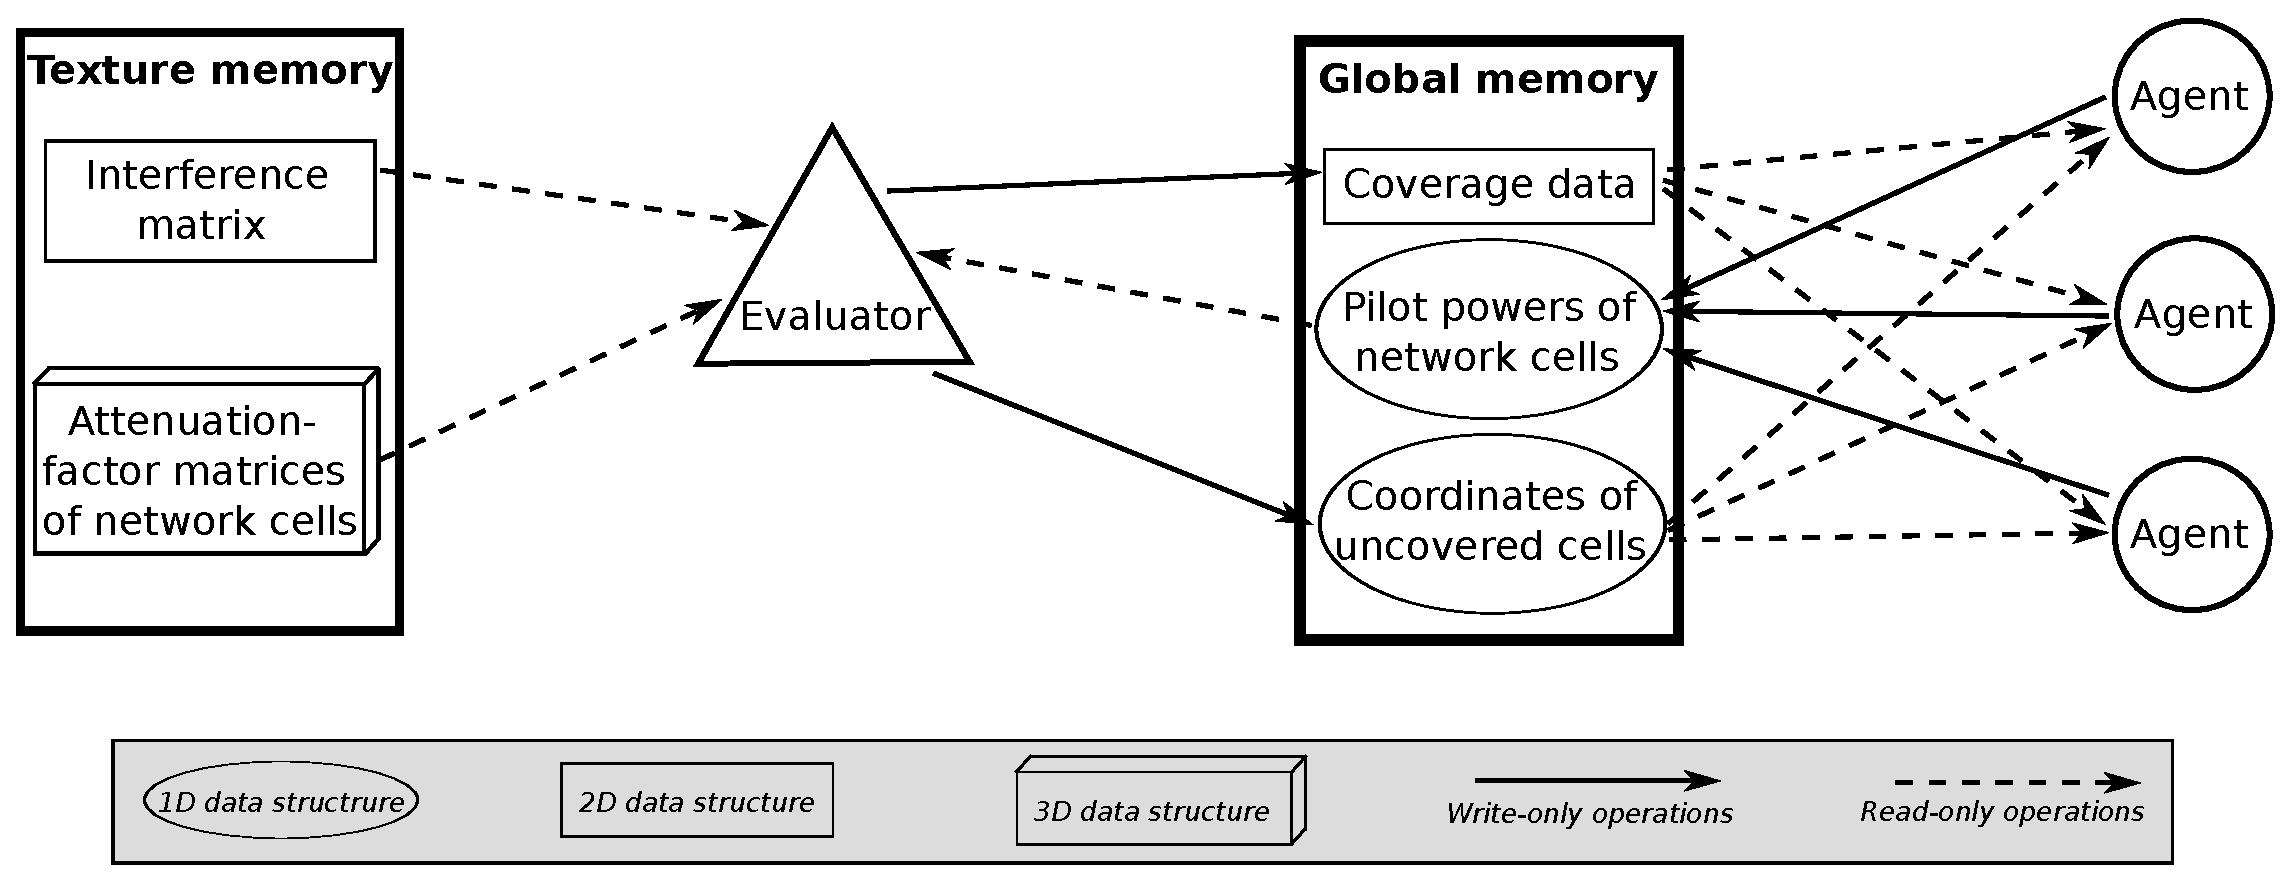
\includegraphics[width=1\textwidth]{06-experimental_evaluation-service_coverage/img/architecture}

\caption{Architecture of the parallel, agent-based optimization system on GPU.\emph{\label{fig:06-Architecture_of_the_system_on_GPU}}}
\end{figure}



\subsubsection{Objective-function evaluation}

The evaluator represents a central component of the optimization system.
It reacts to the pilot-power changes by recalculating the objective-function
value. Recall that the objective-function evaluation involves the
radio-coverage prediction of the service area and the calculation
of the total pilot power used by the cells in the target network.

After a short initialization, during which the attenuation-factor
matrices of all the cells and the interference matrix are calculated,
the evaluator computes the coverage of the service area based on the
pilot powers supplied as the initial solution. Initial solutions are
randomly generated from valid pilot-power settings that conform to
the full coverage constraint.

The evaluator also maintains a special part of the memory (see ``Coordinates
of uncovered cells'' in Figure~\ref{fig:06-Architecture_of_the_system_on_GPU})
that is intended for registering uncovered areas, i.e., $\overline{A_{\mathrm{covered}}}$.
If Equation~(\ref{eq:06-Coverage_constraint}) does not hold, the
``special'' agents randomly select a location from this portion
of memory so that a valid solution may be reached again.

It is worth mentioning that the evaluator itself has no influence
in the optimization process from a quality point-of-view. Its task
is to provide feedback and updated information to the agents that
move through the service area. From a performance point-of-view, the
importance of the evaluator is significant, as it will be shown in
the following sections.

\bigskip{}


The evaluation of the objective function was completely implemented
on the GPU using OpenCL (see Section~\ref{sub:02-OpenCL}). The reason
behind this decision is the impact objective-function evaluation has
on the performance of the optimization system as a whole, as discussed
in Section~\ref{sub:02-Black_box_optimization}. The implementation
of the agents is also based on the GPU, which drastically reduces
the number of data transfers between CPU and GPU, since all problem
elements are available on the GPU during the optimization process.
Consequently, careful memory utilization and organization are critical
to successfully accommodate all involved problem elements on the GPU,
the memory of which is significantly smaller than the RAM available
in desktop computers.


\subsubsection{Autonomous agents}

The agents apply the pilot-power changes only considering local information.
Each of them encapsulates a set of steps that is consistently applied
as it randomly moves through the service area of the network. Whenever
an agent arrives at a new location, the set of covering cells is calculated,
i.e., $C_{m}$.

The step set an agent applies following this point is directly related
to $\vert C_{m}\vert$, whereas its movement is determined by $\vert\overline{A_{\mathrm{covered}}}\vert$,
i.e., the area without service coverage.

The behavior of an agent is dictated by the pseudo-code shown in Algorithm~\ref{alg:07-Agent-behavior}.
The first four steps are responsible for guiding its movements. The
coordinates are randomly selected from two sets, $A_{\mathrm{total}}$
and $\overline{A_{\mathrm{covered}}}$. Only ``special'' agents
may move to a location without service coverage, and they apply the
step set $SS_{0}$ for as long as the solution is not valid. The portion
of ``special'' agents used for correcting a solution is a parameter
of the optimization process. During the following steps of Algorithm~\ref{alg:07-Agent-behavior},
the agent applies step sets $SS_{0}$ and $SS_{1}$ based on the number
of cells in $C_{m}$.

\begin{algorithm}
\centering

\caption{Pseudo-code representing the behavior of an agent.\textit{\label{alg:07-Agent-behavior}}}


\begin{algorithmic}
\Repeat
	\If{$is\_special\_agent()$ $\mathbf{and}$ $\overline{A_{\mathrm{covered}}}>0$}
		\State $l \gets pick\_random\_location(\overline{A_{\mathrm{covered}}})$
	\Else
		\State $l \gets pick\_random\_location(A_{\mathrm{total}})$
	\EndIf
	\State $move(l)$
	\If{$\vert C_{m}\vert=0$}
		\State $apply(SS_{0})$
	\Else
		\If{$\vert C_{m}\vert\ge 1$}
			\State $apply(SS_{1})$
		\EndIf
	\EndIf
\Until{$stopping\_criterion()$}
\end{algorithmic}
\end{algorithm}


If the current location of the agent is not covered by any cell, i.e.,
$\vert C_{m}\vert=0$, the step set $SS_{0}$ is applied (see Algorithm~\ref{alg:07-Agent_step_set_0}).
At the beginning, the cell with the lowest path loss, $c'$, that
may cover a UE at this location, is selected. If several cells have
the same $l_{cm}^{\downarrow}$ value, one of them is randomly chosen.
Once $c'$ is uniquely identified, the agent changes its pilot power
by $inc\_rate$~dB.

\begin{algorithm}
\centering

\caption{Pseudo-code representing the step set $SS_{0}$, which is applied
by the agents in areas without service coverage.\textit{\label{alg:07-Agent_step_set_0}}}


\begin{algorithmic}
\Repeat
	\State $c'\gets cell\_with\_min\_path\_loss(m)$
	\State $p_{c'}\gets adjust\_power(c',inc\_rate)$
\Until{$p_{c'}\in P_{c'}$}
\end{algorithmic}
\end{algorithm}


\begin{algorithm}
\centering

\caption{Pseudo-code representing the step set $SS_{1}$, which is applied
by the agents in areas with service coverage.\label{alg:07-Agent_step_set_1}}


\begin{algorithmic}
\Repeat
	\State $c'\gets pick\_random\_cell(C_{m})$
	\State $p_{c'}\gets adjust\_power(c',dec\_rate)$
\Until{$p_{c'}\in P_{c'}$}
\end{algorithmic}
\end{algorithm}


The step set $SS_{1}$, the pseudo-code of which is listed in Algorithm~\ref{alg:07-Agent_step_set_1},
is applied if the location of the agent is under the coverage of one
or more cells, i.e., $\vert C_{m}\vert\ge1$. The first step randomly
selects a cell from the set $C_{m}$, followed by a decrease of the
pilot power of cell $c'$. Ideally, every pixel of the geographical
area has to be covered by exactly one network cell, although this
is just a representation of a perfect solution that is unreachable
because of irregularities in the network topology and the terrain.

In both step sets, $SS_{0}$ and $SS_{1}$, the agent makes sure that
the new pilot power setting, $p_{c'}$, is an element of $P_{c'}$.
If this is not the case, cell $c'$ is discarded and another cell
is repeatedly selected at the beginning of both step sets, until this
condition is satisfied.

The values $inc\_rate$ and $dec\_rate$ are configurable parameters
that should be set before starting the optimization process. They
indicate the relative adjustment (expressed in dB) of the pilot power
of cell $c'$. On the one hand, lowering the pilot power of a cell
decreases the interference it creates within its coverage area and
those of their neighbors. Since the $\mathrm{SINR}(c,m)$ value increases
with lower interference, the coverage of $m$ may be achieved by a
neighbor cell with the same or lower pilot power. On the other hand,
increasing the pilot power of the cell with the minimum path loss
improves the coverage by evenly distributing the power among different
network cells. This cell is, on average, the nearest one to the location
of a UE $m$.

\bigskip{}


With the objective-function evaluation running on the GPU, a new performance
bottleneck appeared. The limitation factor in this case was the CPU-to-GPU
data transfers that occurred in each iteration of the optimization
process (see Section~\ref{sec:02-CUDA}).

The GPU kernel of the agents is launched as one thread block that
contains one thread per deployed agent. The thread block is organized
in a one-dimensional grid. The initial location of each agent is randomly
generated using the current system time as a random seed. Since OpenCL
provides no function for random-number generation, a simplified version
of Marsaglia's generator~\cite{Marsaglia_Seeds.for.random.number.generator:2003}
was implemented.

The analysis each agent does about the received signals at the current
location is saved into the shared memory of the thread block. It contains
the network cell and its pilot-power setting. Since both numbers are
of type \emph{short}, each of which takes up two bytes, there is enough
space in a 16~KB shared-memory block to allocate 4,096 agents. The
last step involves saving the new pilot powers into global memory.
This step is performed by only one of the threads within the thread
block in order to avoid memory-access conflicts. Updated pilot powers
are saved in negative form to indicate that coverage re-calculation
is needed for these cells. In case there are several updated pilot
powers for one network cell, the median is calculated and applied
as the new pilot power.

Even though coalesced access is not achieved by the GPU kernel of
the agents, its sole implementation provided enhanced performance.
This performance gain appears because of the lower number of data
transfers between the CPU and the GPU, since most data are available
in global memory. Moreover, the GPU kernel also produces the truly
parallel behavior of the agents, as they all apply the pilot-power
changes at the same time.


\section{Simulations \label{sec:06-Simulations}}


\subsection{Test networks}

The test networks, Net$_{1}$, Net$_{2}$ and Net$_{3}$, are subsets
of the real radio network deployed by Telekom Slovenije, d.d. The
path-loss predictions were calculated using the radio-propagation
model presented in Section~\ref{sub:04-Radio_propagation_model}.
A DEM with a 25~m$^{2}$ resolution was used as the terrain-profile
data. The requirements for the coverage threshold, $\gamma^{\mathrm{cov}}$,
were provided by experts of the Radio Network department of Telekom
Slovenije, d.d.

Net$_{1}$ is deployed over a densely populated urban area. For this
reason, the value of $\gamma^{\mathrm{cov}}$ is lower here, since
network capacity is the dominating factor, whereas coverage is flexible
because of a larger cell density, i.e., more BSs per surface unit.
Net$_{2}$ represents a network deployed over a rural area, meaning
that the network capacity can be reduced at the cost of a better coverage,
since the user density is lower. The last network, Net$_{3}$, represents
a suburban area with a densely populated, but relatively small, downtown
center, where a compromise between the network capacity and the coverage
has to be achieved.

The second group of test networks, including Net$_{4}$, Net$_{5}$
and Net$_{6}$, is part of the publicly available MOMENTUM project~\cite{Momentum.project}.
Test network Net$_{4}$ represents the city of Berlin (Germany), Net$_{5}$
represents the city of The Hague (Netherlands), and Net$_{6}$ is
the largest network optimized in~\cite{Siomina:Minimum.pilot.power.for.service.coverage},
representing a reduced version of Net$_{4}$. All networks include
information about BS locations, path-loss predictions and realistic
antennas, which are part of the scenarios provided by the MOMENTUM
project.

Network configurations that represent what could be an initial-network
setup by common-planning standards~\cite{WCDMAforUMTS_RadioAccessForThirdGenerationMobileCommunications}
were produced using the attenuation-based approach. Such configurations
can be easily calculated by a network planner. Table~\ref{tab:06-Test_network_sizes}
lists the number of BSs and cells per test network, as well as the
size of the geographical area. Different network-parameter values
used during the simulations are shown in Table \ref{tab:06-Test_network_parameters}.

\begin{table}
\caption{Sizes of the test networks used for experimentation of the service-coverage
problem, in terms of equipment and geographical area.\emph{\label{tab:06-Test_network_sizes}}}


\centering

{\small{}}%
\begin{tabular}{ccccc}
\cmidrule{2-5} 
 & {\small{Number of base stations}} & {\small{Number of cells}} & {\small{Surface {[}km$^{2}${]}}} & {\small{Resolution {[}m$^{2}${]}}}\tabularnewline\addlinespace
\midrule
{\small{Net$_{1}$}} & {\small{26}} & {\small{77}} & {\small{100.00}} & {\small{25}}\tabularnewline
{\small{Net$_{2}$}} & {\small{8}} & {\small{23}} & {\small{306.25}} & {\small{25}}\tabularnewline
{\small{Net$_{3}$}} & {\small{45}} & {\small{129}} & {\small{405.00}} & {\small{25}}\tabularnewline
{\small{Net$_{4}$}} & {\small{65}} & {\small{193}} & {\small{56.25}} & {\small{50}}\tabularnewline
{\small{Net$_{5}$}} & {\small{12}} & {\small{36}} & {\small{16.00}} & {\small{50}}\tabularnewline
{\small{Net$_{6}$}} & {\small{50}} & {\small{148}} & {\small{56.25}} & {\small{50}}\tabularnewline
\bottomrule
\end{tabular}
\end{table}


\begin{table}
\caption{Network parameters of the test networks used for the service-coverage
problem.\emph{\label{tab:06-Test_network_parameters}}}


\centering

\begin{tabular}{cccc}
\cline{2-4} 
 & $p_{c}^{k}$ & $\mathrm{N}_{0}$ & $\gamma^{\mathrm{cov}}$\tabularnewline
\hline 
Net$_{1}$ & 15.00 W & 1.55$\cdot10^{-14}$ W & 0.010\tabularnewline
Net$_{2}$ & 19.95 W & 1.55$\cdot10^{-14}$ W & 0.020\tabularnewline
Net$_{3}$ & 15.00 W & 1.55$\cdot10^{-14}$ W & 0.015\tabularnewline
Net$_{4}$ & 19.95 W & 1.55$\cdot10^{-14}$ W & 0.010\tabularnewline
Net$_{5}$ & 19.95 W & 1.55$\cdot10^{-14}$ W & 0.010\tabularnewline
Net$_{6}$ & 19.95 W & 1.55$\cdot10^{-14}$ W & 0.010\tabularnewline
\hline 
\end{tabular}
\end{table}



\subsection{Parameter settings of the parallel-agent approach \label{sub:06-Algorithm_parameter_settings}}

The parameter settings for the optimization algorithm were determined
after some experimentation with the test networks. The parameter settings
for each test networks are listed in Table~\ref{tab:06-Parameter_settings}.

\begin{table}
\caption{Parameter settings of the parallel-agent approach for each test network.\emph{\label{tab:06-Parameter_settings}}}


\centering

\begin{tabular}{ccccc}
\cmidrule{2-5} 
 & Agents & $inc\_rate$ {[}dB{]} & $dec\_rate$ {[}dB{]} & Pilot-power changes\tabularnewline\addlinespace
\midrule
Net$_{1}$ & 16 & 0.2 & -0.1 & 10,000\tabularnewline
Net$_{2}$ & 16 & 0.2 & -0.1 & 10,000\tabularnewline
Net$_{3}$ & 16 & 0.2 & -0.1 & 10,000\tabularnewline
Net$_{4}$ & 6 & 1.0 & -0.1 & 10,000\tabularnewline
Net$_{5}$ & 2 & 1.0 & -0.1 & 10,000\tabularnewline
Net$_{6}$ & 6 & 1.0 & -0.1 & 10,000\tabularnewline
\bottomrule
\end{tabular}
\end{table}


Using a higher $inc\_rate$ than $dec\_rate$ reflects the behavior
of the agents when full coverage of the service area is not guaranteed.
In practice, areas without service coverage usually appear as irregular
islands. The stopping criteria were set by limiting the total number
of pilot-power changes an agent is allowed to make. The value was
set to 10,000, even though for some of the test networks the best
solutions were found in the first quarter of the experiment.

\bigskip{}


All experiments were performed on a multi-core Intel i7 2.67~GHz
desktop computer with 6~GB of RAM running a 64-bit Linux operating
system. The GPU hardware used was an nVidia GeForce GTX~660~Ti.
The implementation language used was C, combined with OpenCL and OpenMPI
extensions.


\subsection{Results}

The results achieved by the parallel-agent approach, which are listed
in Table~\ref{tab:06-Optimization_results}, improved the optimization
objective significantly. They show that the pilot-power usage was
reduced in all networks while the service area was kept under full
coverage. Moreover, the parallel-agent solution for Net$_{1}$ improved
the attenuation-based setting by more than 300~\%. As for Net$_{2}$,
the observed improvement is around 232~\%, while the improvement
for Net$_{3}$ is more than 170~\%. 

The last test network, Net$_{6}$, is the same as N6 in~\cite{Siomina:Minimum.pilot.power.for.service.coverage}.
When comparing these results to those of~\cite{Siomina:Minimum.pilot.power.for.service.coverage},
an improvement of almost 3~\% can be observed in the solution provided
by the parallel-agent approach, i.e., 0.778 against 0.759 for the
average pilot power of Net$_{6}$.

\begin{table}
\caption{Optimization results after applying two different approaches for solving
the service-coverage problem. All values are expressed in Watts.\emph{\label{tab:06-Optimization_results}}}


\centering

\begin{tabular}{crccrc}
\cmidrule{2-6} 
 & \multicolumn{2}{c}{Attenuation-based} &  & \multicolumn{2}{c}{Parallel agents}\tabularnewline\addlinespace
\cmidrule{2-3} \cmidrule{5-6} 
 & Total power & Average pilot power &  & Total power & Average pilot power\tabularnewline\addlinespace
\cmidrule{1-3} \cmidrule{5-6} 
Net$_{1}$ & 419.292 & 5.445 &  & 137.064 & 1.780\tabularnewline
Net$_{2}$ & 78.297 & 3.404 &  & 33.344 & 1.450\tabularnewline
Net$_{3}$ & 1,014.113 & 7.861 &  & 582.954 & 4.519\tabularnewline
Net$_{4}$ & 179.876 & 0.932 &  & 145.715 & 0.755\tabularnewline
Net$_{5}$ & 73.872 & 2.052 &  & 34.884 & 0.969\tabularnewline
Net$_{6}$ & 147.014 & 0.993 &  & 112.332 & 0.759\tabularnewline
\bottomrule
\end{tabular}
\end{table}



\subsection{Performance analysis}

The graphs shown in Figures~\ref{fig:06-Convergence_Net1}, \ref{fig:06-Convergence_Net2}
and~\ref{fig:06-Convergence_Net3} depict the convergence of the
parallel-agent approach after ten independent runs for test networks
Net$_{1}$, Net$_{2}$ and Net$_{3}$, respectively. Only feasible
solutions were plotted, i.e., the solutions that meet the full-coverage
constraint. Unfeasible solutions were marked with a value of inferior
quality than the worst solution found: 428 for Net$_{1}$, 129 for
Net$_{2}$, and 1,435 for Net$_{3}$.

From the graphs of Net$_{1}$ (see Figure~\ref{fig:06-Convergence_Net1})
and Net$_{2}$ (see Figure~\ref{fig:06-Convergence_Net2}), a good
initial convergence can be observed. This is followed by a steady
improvement of the intermediate solutions. In Net$_{1}$, no additional
solution improvement is noticed towards the end of the optimization
process. This fact suggests that the stopping criteria is suitable
for this problem instance. A similar situation is observed for Net$_{2}$
that also shows a flat profile towards the end. From the graph of
Net$_{3}$ (see Figure~\ref{fig:06-Convergence_Net3}), a slower
initial convergence, followed by a steady improvement of intermediate
solutions and no significant solution enhancement towards the end,
can be observed. This convergence profile suggests that this problem
instance presents a more difficult optimization case than for Net$_{1}$
and Net$_{2}$. Indeed, this is the largest test network in terms
of surface area. However, further investigation is needed to confirm
this hypothesis. Nevertheless, the parallel-agent approach improved
the pilot-power usage of this test network by almost 75~\%.

\begin{figure}[h]
\centering

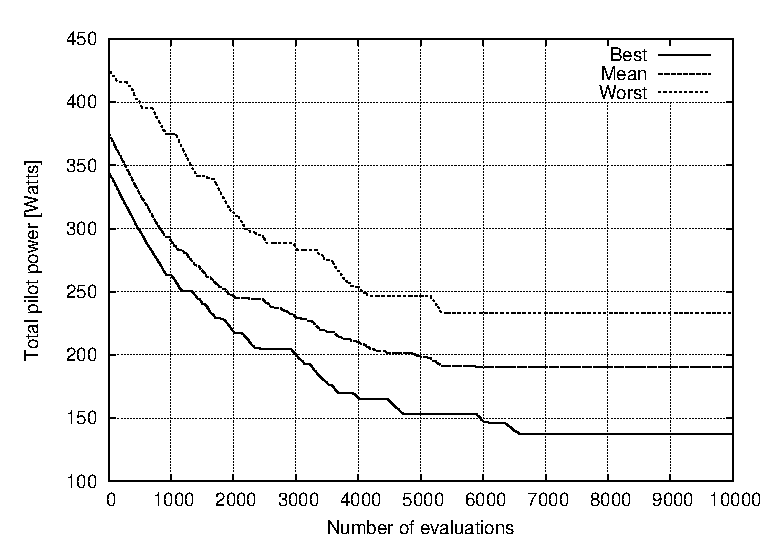
\includegraphics[width=0.7\textwidth]{06-experimental_evaluation-service_coverage/img/convergence_first}

\caption{Convergence profile of the parallel-agent approach for the test network
Net$_{1}$, deployed over an urban area.\emph{\label{fig:06-Convergence_Net1}}}
\end{figure}


\begin{figure}[h]
\centering

\includegraphics[width=0.7\textwidth]{06-experimental_evaluation-service_coverage/img/convergence_second}

\caption{Convergence profile of the parallel-agent approach for the test network
Net$_{2}$, deployed over a rural area.\emph{\label{fig:06-Convergence_Net2}}}
\end{figure}


\begin{figure}[h]
\centering

\includegraphics[width=0.7\textwidth]{06-experimental_evaluation-service_coverage/img/convergence_third}

\caption{Convergence profile of the parallel-agent approach for the test network
Net$_{3}$, deployed over a suburban area.\emph{\label{fig:06-Convergence_Net3}}}
\end{figure}


\bigskip{}


In the following, the speed-performance analysis of the experimental
simulations is presented. This analysis covers the running times during
the optimization of the first three test networks, i.e., Net$_{1}$,
Net$_{2}$ and Net$_{3}$. The running times were measured for each
implementation, and the average times, calculated after ten independent
runs, are given. The number of pilot-power changes per agent was limited
to 1,000, while all other algorithm parameters were kept at the same
values as in Section~\ref{sub:06-Algorithm_parameter_settings}.

Table~\ref{tab:06-Performance_analysis} lists the average wall-clock
times in seconds for the different implementations and test networks.
The implementations include: the CPU-MPI implementation that consists
of objective-function evaluation on CPU and parallel agents over MPI,
the GPU-MPI implementation that consists of objective-function evaluation
on GPU and parallel agents over MPI, and the GPU-GPU implementation
that consists of objective-function evaluation and parallel agents
on the same GPU. The CPU-MPI implementation is the basis for the speedup
calculation of the other two implementations.

The function evaluation on the GPU that communicates with the agents
over MPI provides the second measured setup. The evaluator implementation
takes advantage of shared memory for thread collaboration within a
thread block and texture memory for constant elements, as is it was
explained in Section~\ref{sub:04-GPU_worker_implementation}. Still,
the speedup is considerable but improvable, since numerous data transfers
between CPU and GPU are needed for the agents to access optimization-related
information. The last result set presents measurements for the complete
GPU implementation, including objective-function evaluation and agents
on the same device. The improved speedup delivered by this combination
highlights the impact that CPU-to-GPU memory transfers have on the
overall system performance. This fact is supported by the second and
third measured setups, the speedups of which exhibit, on average,
a four-fold improvement. It is also interesting to note how the speedup
gain increases with the problem-instance size. This fact confirms
that larger problem instances have a greater benefit from a parallel
implementation in terms of computational time.

\begin{table}
\caption{Wall-clock times (in seconds) and speedup factors for the different
implementations of the objective-function evaluation and the parallel
agents, as measured during the experimentation of the service-coverage
problem.\label{tab:06-Performance_analysis}}


\centering

\begin{tabular}{cccccccc}
\cmidrule{2-8} 
 & \multicolumn{1}{c}{CPU-MPI} &  & \multicolumn{2}{c}{GPU-MPI} &  & \multicolumn{2}{c}{GPU-GPU}\tabularnewline\addlinespace
\cmidrule{2-2} \cmidrule{4-5} \cmidrule{7-8} 
 & Avg. time {[}s{]} &  & Avg. time {[}s{]} & Speedup &  & Avg. time {[}s{]} & Speedup\tabularnewline\addlinespace
\cmidrule{1-2} \cmidrule{4-5} \cmidrule{7-8} 
Net$_{1}$ & 4,105 &  & 872 & 4.71 &  & 206 & 19.93\tabularnewline
Net$_{2}$ & 774 &  & 304 & 2.55 &  & 124 & 6.24\tabularnewline
Net$_{3}$ & 5,981 &  & 1,283 & 4.66 &  & 249 & 24.02\tabularnewline
\bottomrule
\end{tabular}
\end{table}



\section{Summary}

This chapter presented a novel optimization approach for solving the
well-known service-coverage problem in radio networks. The problem
addressed the full coverage of a geographical area using a minimum
amount of pilot power. The newly introduced parallel-agent approach
was successfully tested in six networks that represent real-world
scenarios. The experimental results show that the parallel-agent approach
is able to find better solutions than some heuristics, like the presented
attenuation-based approach. Moreover, the algorithm successfully tackled
larger networks, thus overcoming the obstacles of other state-of-the-art
optimization methods regarding problem-instance size~\cite{Siomina_Pilot.power.optimization:2004,Siomina:Minimum.pilot.power.for.service.coverage}.

Compared to a different optimization approach in the literature~\cite{Siomina:Minimum.pilot.power.for.service.coverage},
the solution-quality of the parallel-agent approach showed a quality
improvement. The proposed solutions, calculated for the same problem
instance as in~\cite{Siomina:Minimum.pilot.power.for.service.coverage},
were improved at the cost of a longer running time. It is worth mentioning
that it is feasible for the optimization algorithm to take a longer
time to reach the solution, since design problems, as the service-coverage
one, are usually solved offline. A comparison and analysis of the
performance of the radio-coverage prediction for real-world, radio-network
planning is later provided in Chapter~\ref{chap:08-Real-world_network_planning}.

Different implementations of the parallel-agent approach, combining
a serial version on CPU, parallel processes over MPI and GPU kernels,
were presented. In particular, GPU architectures enable the implementation
of parallel heuristics in a natural way while substantially improving
the computational-time performance. To the best of the author's knowledge,
the parallel-agent approach as presented in this chapter, has not
yet been described in the related literature.

\cleardoublepage{}


\chapter{Experimental evaluation: the SHO alignment problem \label{chap:Experimental-evaluation-the-SHO-alignment-problem}}

% First paragraph has no indentation.

\noindent This chapter introduces a static network simulator to find
downlink and uplink SHO areas. By introducing a penalty-based objective
function and some hard constraints, we formally define the problem
of balancing SHO areas in UMTS networks. The state-of-the-art mathematical
model used and the penalty scores of the objective function are set
according to the configuration and layout of a real mobile network,
deployed in Slovenia by Telekom Slovenije, d.d.. The balancing problem
is then tackled by three optimization algorithms, each of them belonging
to a different category of metaheuristics. We report and analyze the
optimization results, as well as the performance of each of the optimization
algorithms used.


\section{Introduction and motivation \label{sec:Introduction}}

In mobile networks, handover is one of the main features that allows
user's mobility \cite{WCDMAforUMTS_RadioAccessForThirdGenerationMobileCommunications}.
The concept behind the handover operation is simple: when a user moves
from the coverage area of a cell to the coverage area of a neighboring
cell, the system creates a new connection with the latter cell and
disconnects the user from the former one, while keeping the current
connection active. Soft-handover (SHO), on the other hand, is a possibility
available in mobile networks using the Wideband Code Division Multiple
Access (WCDMA) technology, which the Universal Mobile Telecommunications
System (UMTS) employs. SHO enhances handover functionality by allowing
a user to potentially operate on multiple radio links in parallel.
Since different users are separated by unique spreading codes, the
detection of single user's signal is implemented by despreading with
the same code sequence used in the transmitter \cite{WCDMAforUMTS_RadioAccessForThirdGenerationMobileCommunications}.

Every mobile terminal constantly monitors the common pilot power channel
(CPICH) of the connected cell and its neighbors. The information about
these measurements is sent to the network by the user terminal (i.e.
mobile). The SHO condition depends on the relative received signal
quality from different cells and the SHO window, which triggers the
addition of a cell to the user's active set. Depending on radio propagation
characteristics and different transceiver capabilities, the radio
transmission can gain more than 3 dB out of a SHO situation \cite{WCDMAforUMTS_RadioAccessForThirdGenerationMobileCommunications}.
From this point of view, SHO is a method to reduce interference and
improve radio quality, particularly at the cell border where radio
coverage is of inferior quality. In UMTS Release 99 \cite{3GPP_R99},
SHO is specified to work from the network towards the user (i.e. downlink),
and from the user towards the network (i.e. uplink).

With the introduction of High Speed Packet Access (HSPA) as an improvement
of the performance existing in WCDMA protocols, the role SHO plays
in mobile network configuration and functioning slightly changed.
The key difference is that High Speed Downlink Packet Access (HSDPA)
does not support SHO, while the High Speed Uplink Packet Access (HSUPA)
does. This particular distinction has some key implications in the
balanced distribution of SHO areas, and thus in the quality of HSPA
services \cite{holma2006hsdpa}.



\begin{figure*}[tp]
\centering

\includegraphics[width=3.7in]{07-experimental_evaluation-sho_balancing/img/network_normal}\includegraphics[width=3.7in]{07-experimental_evaluation-sho_balancing/img/network_problem}\\\vskip -0.3in(a)\hspace*{3.6in}(b)

\caption{HSUPA traffic and uplink interference with: (a) balanced downlink
and uplink SHO conditions; (b) unbalanced downlink and uplink SHO
conditions.\label{fig:problem_illustration}}
\end{figure*}


Despite several built-in mechanisms that allow the network to overcome
different problems due to the lack of SHO during a HSDPA connection,
some abnormal cases do arise, especially in those areas where there
is SHO capability in the uplink, but none in the downlink. An example
of such a case is depicted in Figure \ref{fig:problem_illustration},
which shows interference behavior during a HSPA connection in normal
SHO conditions (a), and in unbalanced SHO conditions (b). Graph data
are actual radio network statistics, taken from the mobile network
deployed in Slovenia by Telekom Slovenije, d.d.. The graph on the
left (a) shows a normal HSUPA-enabled service situation, in which
the measured interference is proportional to the traffic being served.
Note how the noise rises with the increased traffic on cell 1, while
its neighbor (cell 2) has almost no interference nor traffic. Moreover,
the graph profile for both traffic and noise of cell 1 are almost
identical. The graph on the right (b) depicts a problematic situation,
where the noise level does not only rise on the cell serving the HSUPA
services (cell 1), but also on the neighboring one. Notice how the
interference level rises on the cell that has almost no traffic (cell
2). It is clear that the source of this noise rise is generated by
the active connection on cell 1, which shows an increase in HSUPA
traffic. However, the noise level profile on cell 2 does not follow
its traffic, as it did in the normal situation (a). This is due to
cell 2 not being part of the active set. Such situations appear when
the UL coverage is larger than the DL coverage. Interestingly enough,
this seems to be an exceptional case, as Holma and Toskala write in
\cite{holma2006hsdpa} when describing soft handover in Chapter 5:

''... There is no obvious reason why the serving E-DCH cell would
not be the same as the serving HSDPA cell, and this is also required
to be the case in the specifications.''

Given the described context, the challenge is to achieve the correct
balance or distribution of downlink and uplink SHO areas within a
working UMTS network. Therefore, the network has to be fine-tuned
to achieve a better SHO-area balancing, and thus avoiding the appearance
of problematic situations as shown in Figure \ref{fig:problem_illustration}.
This clearly implies that the mobile network configuration should
not be excessively altered, since other aspects of the network are
working well before starting the optimization process. Hence, we have
decided to define an optimization problem which objective is to find
a CPICH power level configuration for all the cells in the working
network, such that the balance of downlink and uplink SHO areas is
improved and other network aspects are preserved. The optimization
process takes into account different kinds of hardware (e.g. amplifiers,
cables, and antennas), but only the CPICH powers of the cells are
to be changed.

In this paper we utilize a static network simulator, based on a state-of-the-art
mathematical model \cite{nawrocki2006understanding}, to find downlink
and uplink SHO areas. By introducing a penalty-based objective function
and some hard constraints, we formally define the problem of balancing
SHO areas in UMTS networks. The mathematical model and the penalty
scores of the objective function are set according to the configuration
and layout of a real mobile network, deployed in Slovenia by Telekom
Slovenije, d.d.. The SHO settings are also taken from actual network
configuration, still they were adapted to closely model interference
and other dynamics present in the network. The balancing problem is
then tackled by three optimization algorithms, each of them belonging
to a different category of metaheuristics. The optimization results,
as well as the performance of each of the optimization algorithms
used, are afterwards analyzed.

The remainder of this paper is organized as follows: in Section \ref{sec:Related-work-1}
we give an overview of other works related to CPICH-power and SHO
optimization in UMTS. The static network model is presented in Section
\ref{sec:Static_network_model}, where all the elements of the mathematical
model and the objective function are defined. In Section \ref{sec:Optimization-algorithms}
we introduce and shortly describe the optimization algorithms used
to tackle the balancing problem. The simulations, including their
environment and parameter setup, are described in Section \ref{sec:Simulations-1},
followed by their results in Section \ref{sec:Results}. We conclude
with Section \ref{sec:Conclusion} by giving a conclusion and guides
for future work.




\section{Related work \label{sec:Related-work-1}}

SHO optimization has received quite some attention from the scientific
community in the last years. This mainly relates to the importance
it has within deployed networks that provide high speed services such
as video telephony \cite{chen2010_impact_of_soft_handover} and Internet
access by means of HSPA \cite{chen2011_coverage_planning_for_optimizing_HSDPA}.

Some authors tackle optimization problems at the planning stage of
the network \cite{Eisenblatter_OptimizationMethodsForUMTSRadioNetworkPlanning,ghosh2011_optimising_CDMA_cell_planning},
considering, among other variables, base station locations and hardware.
The fact is that most mobile operators are unable to apply these contributions
to a live network since the planning phase has long been concluded.
Moreover, the great majority of the base stations have already been
deployed and their hardware also installed. Therefore, from the mobile
operator's point of view, mainly parameter and software optimization
are the tools available when it comes to improvement of the quality
of service and troubleshooting the network in the short term.

Optimizing SHO by means of CPICH is an established way of enhancing
network capacity when high speed services like HSDPA an HSUPA coexist
with legacy technologies \cite{chen2008cpich}. The CPICH transmit
power is typically between 5\% to 10\% of the total downlink transmit
power of the base station \cite{RadioNetworkPlanningAndOptimisationForUMTS},
but there is no standardized method to fi{}nd a CPICH power setting.
A number of existing approaches to resolve this issue exist in the
related literature (see \cite{WCDMAforUMTS_RadioAccessForThirdGenerationMobileCommunications,Siomina_PilotPowerManagementInWCDMANetworksCoverageControlWithRespectToTrafficDistribution,Ying_CPICHPowerSettingsInIrregularWCDMAMacroCellularNetworks}).
The most eff{}ective ones are those based on optimization methods
\cite{Eisenblatter_OptimizationMethodsForUMTSRadioNetworkPlanning,GarciaLozano_CPICHPowerOptimisationByMeansOfSimulatedAnnealingInAnUTRAFDDEnvironment,RadioNetworkPlanningAndOptimisationForUMTS,UMTSRadioNetworkPlanning_OptimizationAndQoSManagementForPracticalEngineeringTasks,siomina2008minimum}.
Such a wide spectrum of proposed procedures is directly related to
the diverse criteria taken into account when assigning the CPICH power
of a cell. The fundamental reason behind this fact is that the CPICH
power is a common factor of various optimization problems in UMTS
networks.

To the best of our knowledge, there is no reference in the literature
to a simulation-based approach to find active downlink and uplink
SHO areas. Additionally, as far as we know, the SHO balancing problem
as described in this paper has not yet been tackled by any formal
optimization method.


\section{Mobile network model \label{sec:Static_network_model}}

Following the representation of a static network model from \cite{nawrocki2006understanding},
this section addresses the definitions of all the elements included
in the mathematical model used for the simulations.

Our goal here is to analyze the state of the network in a given situation,
e.g. a \textquoteleft{}snapshot\textquoteright{} at an arbitrary instance.
A snapshot consists of a set of users (or mobiles) having individual
properties, such as location, and equipment type. The static approach
inherently ignores dynamic effects that influence the system, like
fast power control \cite{nawrocki2006understanding}.

The mathematical model links the SHO settings with CPICH power settings
for each cell, the best-server pattern, and the network coverage.


\subsection{Basic elements}

We start by considering a UMTS network with a set of antenna installations
(cells), $N$. A pixel grid of a given resolution represents the service
area, $A$, within which there is a set of mobiles, $M$. We denote
$L_{im}^{\downarrow}$ as the downlink attenuation factor between
cell $i\in N$ and mobile $m\in M$. Similarly, we define $L_{mi}^{\uparrow}$
as the uplink attenuation factor between mobile $m$ and cell $i$.
The attenuation factor values are calculated by performing signal
propagation predictions for every pair $(i,m)$, $i\in N$, $m\in M$,
using the commercial radio planning tool TEMS$^{TM}$ CellPlanner
\cite{tems}, which is used in the Radio Network Department at Telekom
Slovenije, d.d.. These predictions already include losses and gains
from cabling, hardware, and user equipment.

By introducing a change step of 0.01~dB and bounding the CPICH power
of a cell $i$ to $\pm2$~dB, relative to the CPICH power setting
the cell had before optimization, we define a finite set of candidate
CPICH power settings for cell $i$ as $P_{i}=\{p_{i}^{1},p_{i}^{2},...,p_{i}^{K}\}$.
By limiting the possible CPICH power settings a cell $i$ may have,
we are delineating two important aspects of the problem. First, since
we are optimizing a live network, we do not want the algorithms to
create complete new configurations, but just to fine-tune existing
ones. Second, the problem complexity is lowered, because the size
of the search space is smaller.


\subsection{Coverage}

A mobile $m$ within the area $A$ is under network coverage if at
least one cell $i$ covers it. We define the downlink coverage by
means of the received signal code power (RSCP) \cite{WCDMAforUMTS_RadioAccessForThirdGenerationMobileCommunications}.
Following the current network settings, and including a margin for
interference derived from HSDPA \cite{holma2006hsdpa}, the RSCP threshold
is set to -115~dBm ($3.16227766\cdot10^{-12}$~mW). So, for any
pair $(i,m)$, $i\in N$, $m\in M$, the coverage of mobile $m$ by
cell $i$ is defined as

\begin{equation}
cov{}_{im}=\begin{cases}
1 & if\, RSCP_{im}\ge-115\, dBm\\
0 & otherwise
\end{cases}.
\end{equation}


If $m$ is covered by more than one cell, we refer to the cell with
the highest RSCP as the best server, an we denote it as $i^{*}$.


\subsection{SHO areas \label{sub:SHO-areas}}

To obtain a realistic outline of the areas where a mobile may potentially
maintain connections to more than one cell, we use a static version
of the active set \cite{nawrocki2006understanding}. Therefore, we
introduce a SHO window, $\gamma^{\mathrm{SHO}}$, and a \textit{\emph{maximum}}
active set size, $n^{\mathrm{MAX}}$. Both parameters are taken from
the current configuration of the network. The cells to which a mobile
$m\in M$ may maintain concurrent connections are part of the set 



\noindent where $i\in N$, $L_{i^{*}m}^{\downarrow}$ is the downlink
attenuation factor of the cell with the strongest signal (best server),
and $p_{i^{*}}$ is its CPICH power. Since the number of elements
in $SHO_{m}^{\downarrow}$ is at most $n^{\mathrm{MAX}}$, the weakest
links are removed if there are more present. This method is well suited
for configurations with no hysteresis, since dynamic effects are ignored
in static models \cite{nawrocki2006understanding}. 

Additionally, in the uplink, we define the set of cells to which a
mobile can potentially be in SHO as



\noindent where $i\in N$, $L_{mi}^{\uparrow}$ is the uplink attenuation
factor from mobile $m$ to cell $i$, and $P_{m}^{\uparrow}$ is the
uplink transmit power of mobile $m$.

Because of the static nature of the model, we are neglecting mobility
and interference by narrowing the SHO window to 2~dB \cite{nawrocki2006understanding}.


\subsection{Optimization objective}

Using the elements defined in Section \ref{sec:Static_network_model},
we have constructed an objective function in cooperation with a team
of radio engineers of the Radio Network Department at Telekom Slovenije,
d.d.. The objective function is constructed as a weighted sum, containing
different costs that penalize the occurrence of specific SHO conditions
in downlink and uplink, which may potentially cause the aforementioned
malfunctioning, introduced in Section \ref{sec:Introduction}.

A cost-based objective function is the most natural and straight-forward
way of defining the optimization objective. Besides it is easily extendable
to include other future circumstances and it also defines the mutual
importance of the different situations taken into account at the optimization
phase.

Hence, the definition of the objective function for the balancing
problem is the minimization of the sum of penalty scores given as



where 

and
\begin{itemize}
\item $pf_{\mathrm{COV}}$ represents the penalty factor for uncovered areas,
\item $pf_{\mathrm{SHO}}^{\uparrow}$ represents the penalty factor for
uplink SHO areas where SHO is not possible in the downlink, and
\item $pf_{\mathrm{SHO}}^{\downarrow}$ represents the penalty factor for
downlink SHO areas where SHO is not possible in the uplink.
\end{itemize}

\section{Optimization algorithms \label{sec:Optimization-algorithms}}

We tackled the problem of balancing SHO areas using three fundamentally
different optimization algorithms, namely:
\begin{itemize}
\item differential evolution, from the family of evolutionary algorithms;
\item differential ant-stigmergy algorithm, from the family of swarm-intelligence
algorithms; and
\item simulated annealing, from the group of classic metaheuristic algorithms,
targeted at combinatorial optimization problems.
\end{itemize}
Each of these algorithms shall minimize the objective function value
by adopting essentially disparate approaches, hence the diversity
of applying algorithms belonging to different families to solve the
same optimization problem. In this way we want to find out whether
any of the presented approaches is better suited for solving our problem.

In the following sections we give a short introduction about their
functioning and controlling parameters.


\subsection{Differential evolution}

Differential evolution (DE) \cite{storn1997_Differential_evolution}
is a simple and powerful evolutionary algorithm proposed for global
optimization. A wide range of optimization problems have been solved
by applying DE \cite{das2010_differential_evolution_state_of_the_art}.
The algorithm exhibits a parallel direct search method, which utilizes
$D$-dimensional parameter vectors. The balancing problem is expressed
in each component of a vector $X$ of the population, which maps to
the CPICH power of one cell under optimization:

\begin{equation}
X_{aG}=\left\{ x_{1},x_{2},\ldots x_{i},\ldots,x_{D}\right\} ,\label{eq:DE_mapping}
\end{equation}
where $x_{i}\in P_{i}$ represents a candidate CPICH power setting
of cell $i$, and $G$ indicates the generation of an individual $a$
in the population. Since there are $|N|$ cells in the mobile network,
it follows that $D=|N|$.

In each generation, DE produces new parameter vectors by adding the
weighted difference between two population vectors to a third one
\cite{storn1997_Differential_evolution}. The resulting vector is
retained if it yields a lower objective function value than a predetermined
population member; otherwise, the old vector is kept.

There are different variants of DE. We have chosen the most popular
one to solve our optimization problem, called \emph{DE/rand/1/bin}.
The nomenclature used to name this variant indicates the way the algorithm
works:
\begin{itemize}
\item \emph{DE }denotes the differential evolution algorithm,
\item \emph{rand }indicates that the individuals selected to compute the
mutation values are randomly chosen,
\item 1\emph{ }specifies the number of pairs of selected solutions used
to calculate the weighted difference vector, and
\item \emph{bin }means that a binomial recombination operator is used.
\end{itemize}
We considered four parameters to control the search process of DE:
the population size, the maximum number of generations for the algorithm
to run, the crossover constant, and the mutation scaling factor.

An extensive description of DE and its variants may be found in \cite{price2005differential_evolution}.


\subsection{Differential ant-stigmergy algorithm}

Based on the metaheuristic Ant-Colony Optimization (ACO) \cite{dorigo2006ant_colony_optimization},
the differential ant-stigmergy algorithm (DASA) \cite{korosec2010_DASA}
provides a framework to successfully cope with high-dimensional numerical
optimization problems. It creates a fine-grained discrete form of
the search space, representing it as a graph. This graph is then used
as the walking paths for the ants, which iteratively improve the temporary
best solution.

The mapping between the balancing problem and DASA is similar to the
one depicted in Equation (\ref{eq:DE_mapping}):

\begin{equation}
X_{a}=\left\{ x_{1},x_{2},\ldots x_{i},\ldots,x_{D}\right\} \label{eq:DASA_mapping}
\end{equation}


In this case, each ant, $a$, creates its own solution vector, $X_{a}$,
during the minimization process. At the end of every iteration, and
after all the ants have created solutions, they are evaluated to establish
if any of them is better than the best solution found so far.

There are six parameters that control the way DASA explores the search
space: the number of ants, the discrete base, the pheromone dispersion
factor, the global scale-increasing factor, the global scale-decreasing
factor, and the maximum parameter precision.

For a more in-depth explanation about these parameters and the DASA
algorithm itself, we refer the reader to \cite{korosec2010_DASA}.


\subsection{Simulated annealing}

As the third optimization algorithm to tackle the balancing problem
we have chosen simulated annealing (SA) \cite{Kirkpatrick_OptimizationBySimulatesAnnealing},
a classic metaheuristic algorithm often used when the search space
is discrete. SA has proved to be a solid optimization algorithm, capable
of giving high-quality solutions to a wide scope of optimization problems
\cite{Suman_SurveyOfSimulatedAnnealing}.

At each time step during the process, the system under optimization
is in a given \emph{state}. The objective function maps a system state
to a value known as the \emph{energy} of the system in that state.
A \emph{move} in the search space represents a change in the state
of the system. After making a move, the system may exhibit lower or
higher energy, depending on the results of the objective function.
When dealing with minimization problems, a better state always describes
lower energy than the previous one.

SA incorporates the notion of \emph{temperature}, by which the probability
of moving the current state of the system into a worst one is lowered
as the temperature decreases. Exploration of the search space is thus
induced at higher temperature, whereas exploitation appears at lower
temperature, when only improving moves are accepted.

Table \ref{tab:SA_move} shows the pseudo-code of a move in the search
space of possible CPICH power settings, resulting in a new state of
the system.

\begin{table}
\centering

\caption{Pseudo-code: a move in the search space of SA.\textit{\label{tab:SA_move}}}


\begin{tabular}{c|l}
\hline 
Step & \tabularnewline[\doublerulesep]
\hline 
1 & $i'=random\, cell(N)$\tabularnewline
 & $\mathbf{do}$\tabularnewline
2 & $\,\,\, if\, rand()<0.5\, then\, p_{i'}^{\mathrm{NEW}}=p_{i'}+0.01$\tabularnewline
 & $\,\,\, else\, p_{i'}^{\mathrm{NEW}}=p_{i'}-0.01$\tabularnewline
3 & $\mathbf{while}\, p_{i'}^{\mathrm{NEW}}\notin P_{i'}$\tabularnewline
4 & $p_{i'}=p_{i'}^{\mathrm{NEW}}$\tabularnewline
\end{tabular}
\end{table}


At the first step, a cell, $i'$, is randomly selected from the set
of all cells in the network, $N$. In step 2, a change of +0.01~dB
or -0.01~dB is applied with 50\% probability to $p_{i'}$. The current
CPICH power of cell $i'$ is expressed in dBm. The randomly generated
CPICH power setting, $p_{i'}^{\mathrm{NEW}}$, is checked for validity
in step 3, i.e. it must be an element of the set $P_{i'}$. If $p_{i'}^{\mathrm{NEW}}$
is not a valid CPICH power, step 2 is executed again, generating another
random CPICH power. Finally, in step 4, the CPICH power of cell $i$
is replaced by $p_{i'}^{\mathrm{NEW}}$.

It is important to note that, as long as $|P_{i'}|>1$, the algorithm
shown in Table \ref{tab:SA_move} shall never be trapped in an endless
loop. On the other hand, if $|P_{i'}|<2$, there are no candidate
CPICH powers for cell $i'$ and thus no possibility of optimization
by means of CPICH power adjustment.

Notice also that the acceptance of a move in the search space is left
to SA and its stochastic components.


\section{Simulations \label{sec:Simulations-1}}

The simulations are performed using a standard Monte-Carlo method,
assuming the mobile users are uniformly distributed. The path-loss
data were calculated in advance, using the commercial radio planning
tool TEMS$^{TM}$ CellPlanner \cite{tems}. The SHO conditions of
different users depend on the relative received signal quality from
different cells and the SHO window, which triggers the addition of
a cell to the user's active set \cite{WCDMAforUMTS_RadioAccessForThirdGenerationMobileCommunications}.


\subsection{Test network \label{sub:Test-network}}

The test network used for the simulations is a subset of the real
UMTS network deployed in Slovenia by Telekom Slovenije, d.d.. It represents
a network extending over a hilly terrain, combining both rural and
middle-dense suburban areas, which contains 25 cells within an area
of more than 150 $km^{2}$. Table \ref{tab:Test-network-properties.}
shows some properties of the test network used.



\begin{table}
\caption{Test network properties. \label{tab:Test-network-properties.}}


\centering

\begin{tabular}{c|c}
\hline 
Number of cells & $25$\tabularnewline
Coverage threshold (RSCP) & $-115\, dBm$\tabularnewline
SHO window ($\gamma^{\mathrm{SHO}}$) & $2\, dB$\tabularnewline
User equipment ($P_{m}^{\uparrow}$) & $21\, dBm$, power class 4\tabularnewline
Pixel resolution & $25\, m^{2}$\tabularnewline
Population density & $398/km^{2}$\tabularnewline
\hline 
\end{tabular}
\end{table}



\subsection{Penalty factors}

After extensive experimentation, and working in cooperation with the
radio engineers from the Radio Network Department at Telekom Slovenije,
d.d., the penalty factors from Equation (\ref{eq:objective_function})
are set to the following values:
\begin{itemize}
\item $pf_{\mathrm{COV}}=15$,
\item $pf_{\mathrm{SHO}}^{\uparrow}=13$, and
\item $pf_{\mathrm{SHO}}^{\downarrow}=3$.
\end{itemize}
It is clear that coverage is the most important quality aspect from
the network point of view (penalty factor $pf_{\mathrm{COV}}$). Moreover,
it imposes the biggest constraint to the optimization process, since
the balance between SHO areas should not sacrifice network coverage.
Another important characteristic that emerges from these values is
the preference for minimizing areas where SHO capability is available
in the uplink, but not in the downlink (penalty factor $pf_{\mathrm{SHO}}^{\uparrow}$).
As it has been described in Section \ref{sec:Introduction}, one of
the consequences of such SHO arrangement produces serious interference
rise in neighboring cells (Figure \ref{fig:problem_illustration}),
which may also result in service inaccessibility. The last factor
$pf_{\mathrm{SHO}}^{\downarrow}$ imposes a penalty value over areas
where SHO capability is available in the downlink, but not in the
uplink. Remember that when accessing HSPA services, SHO is available
only in the uplink. For this reason, the link throughput may benefit
from SHO in the uplink if it is available. The relative lower importance
of the last penalty factor compared with the other ones is directly
related to the consequences of such unbalancing of SHO areas may have
on the network. In this case only HSPA throughput is affected, while
the service accessibility should not be an issue, given there is enough
uplink coverage \cite{holma2006hsdpa}.


\subsection{Algorithm parameters}

In this section we enumerate the parameters and their values used
during the optimization process. In all three cases we have followed
the naming conventions as they appear in the original publications
\cite{Kirkpatrick_OptimizationBySimulatesAnnealing,korosec2010_DASA,storn1997_Differential_evolution}.


\subsubsection{DE}

The parameters controlling the behavior of the DE algorithm have been
set as follows:
\begin{itemize}
\item $NP=100$, the population size;
\item $G_{max}=1000$, the maximum number of generations for the algorithm
to run;
\item $CR=0.8$, the crossover constant; and
\item $F=0.5$, the mutation scaling factor.
\end{itemize}

\subsubsection{DASA}

As for DASA, we have set the parameters to the following values:
\begin{itemize}
\item $m=10$, the number of ants;
\item $b=10,$ the discrete base;
\item $q=0.2$, the pheromone dispersion factor;
\item $s_{+}=0.01$, the global scale-increasing factor;
\item $s_{-}=0.01$, the global scale-decreasing factor; and 
\item $e=1.0^{-2}$, the maximum parameter precision.
\end{itemize}

\subsubsection{SA}

There are only two parameters controlling SA, the initial temperature
and the total number of iterations or evaluations:
\begin{itemize}
\item $t_{initial}=125$,
\item $it=100,000$.
\end{itemize}
SA also allows to define the way the temperature is lowered during
the annealing process. In this case, we have used the exponential-lowering
schema.


\subsection{Experimental environment}

All experiments were carried out on a 4-core Intel i7 2.67~GHz desktop
computer with 6~GB of RAM running a 64-bit Linux operating system.
The implementation languages used were C and Python, with the latter
mostly used as \textquoteleft{}glue\textquoteright{} to hold the different
implementation parts together, as well as for I/O operations. To lower
the time needed to run one optimization round, we have implemented
the entire objective function evaluation using OpenCL and executed
it on a nVidia GeForce GTX 260. This individual improvement exhibited
more than 15x execution time speed-up when compared to the original
CPU-only version.


\section{Results \label{sec:Results}}


\subsection{Algorithm performance}

In this section we examine the performance of the three selected algorithms
in terms of solution quality and convergence speed. All experimental
results were obtained after 30 independent runs, each of them limited
to a maximum of 100,000 evaluations. The gathered results are shown
in Table~\ref{tab:algorithm_performance}.

\begin{table}
\centering

\caption{Algorithm performance after 30 runs\textit{\emph{.}}\textit{\label{tab:algorithm_performance}}}


\begin{tabular}{ccccc}
\toprule 
 & Best & Worst & Mean & Std. deviation\tabularnewline\addlinespace
\midrule
DE & 2,286,292.00 & 2,286,541.00 & 2,286,517.09 & 62.06\tabularnewline
DASA & 2,286,446.00 & 2,286,633.00 & 2,286,592.00 & 26.19\tabularnewline
SA  & 2,293,350.00 & 2,295,570.00 & 2,294,626.50 & 663.75\tabularnewline
\bottomrule
\end{tabular}
\end{table}




As we may observe, DE reaches the lowest objective function value,
closely followed by DASA. Likewise, both algorithms reach very similar
results for the worst, mean and standard deviation values. SA, on
the other hand, did not achieve similar values, since its results
are behind those of DE and DASA. Notice that even the best SA solution
is no better than the worst solution of DASA. Moreover, the standard
deviation exhibited by SA is many times bigger to those of DASA and
DE, inducing the greater level of variance of its results.

\begin{figure}
\centering

\includegraphics[width=1\columnwidth]{07-experimental_evaluation-sho_balancing/img/convergence}\\\vskip -0.3in

\caption{Algorithm convergence for the best obtained results.\label{fig:algorithm_convergence}}
\end{figure}


\begin{table*}
\centering

\caption{Optimization results.\textit{\label{tab:optimization-results}}}


\begin{tabular}{ccccccc}
\toprule 
 & Uncovered area & Covered area, no SHO & Normal SHO area & no SHO$^{\downarrow}$, SHO$^{\uparrow}$ & SHO$^{\downarrow}$, no SHO$^{\uparrow}$ & Total\tabularnewline\addlinespace
\midrule
Before optimization & 63.00 \% & 15.11 \% & 15.73 \% & 1.80 \% & 4.36 \% & 100.00 \%\tabularnewline
\cmidrule{2-7} 
DE solution & 60.23 \% & 16.13 \% & 16.09 \% & 1.47 \% & 6.08 \% & 100.00 \%\tabularnewline
DASA solution & 60.24 \% & 16.16 \% & 16.90 \% & 1.46 \% & 5.24 \% & 100.00 \%\tabularnewline
SA solution & 60.42 \% & 16.55 \% & 15.97 \% & 1.56 \% & 5.50 \% & 100.00 \%\tabularnewline
\cmidrule{2-7} 
DE improvement & +4.40 \% & +6.75 \% & +2.29 \% & +18.33 \% & -39.45 \% & ---\tabularnewline
DASA improvement & +4.38 \% & +6.95 \% & +7.44 \% & +18.88 \% & -20.18 \% & ---\tabularnewline
SA improvement & +4.09 \% & +9.53 \% & +1.52 \% & +13.33 \% & -26.15 \% & ---\tabularnewline
\cmidrule{2-7} 
Avg. improvement & +4.29 \% & +7.74 \% & +3.75 \% & +16.85 \% & -28.59 \% & ---\tabularnewline
\bottomrule
\end{tabular}
\end{table*}


\begin{figure*}
\centering

\begin{minipage}[t]{0.5\textwidth}%
\centering

\includegraphics[width=1\textwidth]{07-experimental_evaluation-sho_balancing/img/sho_areas_initial}\vskip -0.3in

\caption{Spatial distribution of SHO areas, before optimization.\label{fig:sho_areas_initial}}
%
\end{minipage}\hfill{}%
\begin{minipage}[t]{0.5\textwidth}%
\centering

\includegraphics[width=1\textwidth]{07-experimental_evaluation-sho_balancing/img/sho_areas_final}\vskip -0.3in

\caption{Spatial distribution of SHO areas, after optimization.\label{fig:sho_areas_final}}
%
\end{minipage}
\end{figure*}


The convergence of the best-recorded run of each of the three algorithms
is shown in Figure \ref{fig:algorithm_convergence}. It is worth mentioning
that every optimization run starts from a different solution, randomly
constructed by picking a CPICH power setting, $p_{i}^{k}$, from every
$P_{i}=\{p_{i}^{1},p_{i}^{2},...,p_{i}^{K}\}$, $1\le k\le|P_{i}|$,
$\forall i\in N$. Notice how fast DASA converges to a good solution.
After a number of evaluations without improvement, DASA resets itself
and continues searching from a new random point within the search
space \cite{korosec2010_DASA}, hence the jagged profile on the graph.
Similarly, DE converges considerably fast, although not as fast as
DASA does. It this case, DE does not reset itself if the current solution
cannot be improved. Despite this, and based on the flat profile the
graph exhibits towards the end of the optimization run, we are confident
that 100,000 evaluations is an adequate stopping criterion for this
algorithm. The last algorithm, SA, slowly converges towards the best
solution found, even though it is not as good as the solutions found
by DE and DASA. 

The three convergence profiles shown in Figure \ref{fig:algorithm_convergence}
give a clearer notion about the way these algorithms explore the search
space of the balancing problem.

Running times of the algorithms are intentionally omitted, since the
implementations used are fundamentally different and therefore not
comparable.


\subsection{Interpretation}

Table \ref{tab:optimization-results} presents the analysis of the
obtained results from the network point of view. After 30 independent
runs of each of the three algorithms, the best results obtained where
evaluated for improvement and decline of each of the measured network
aspects. The results are shown in Table \ref{tab:optimization-results},
where '+' indicates improvement and '-' indicates decline of the given
criteria. We may observe that the measured criteria have been significantly
improved. The only exception is the measure labeled as \textquoteleft{}SHO$^{\downarrow}$,
no SHO$^{\uparrow}$\textquoteleft{}, which shows an expected change,
since it is the optimization aspect with the lowest penalty factor
value.

Coverage has been improved with an average of 4.29\%, whereas the
coverage area where there is no SHO capability has been increased
7.74\% in average. The SHO areas, where this facility is available
in both the downlink and uplink, has also been improved 3.75\% in
average. This particular improvement is interesting from the optimization
point of view, because it had no explicit penalty factor set. Therefore
we understand this enhancement as a consequence of the completeness
of criteria, taken into account in the objective function.

The second most important optimized aspect in the balancing problem
is the proportion of areas with uplink SHO and no SHO in the downlink
(labeled as \textquoteleft{}no SHO$^{\downarrow}$, SHO$^{\uparrow}$\textquoteleft{}
in Table \ref{tab:optimization-results}). This particular condition
has been improved by almost 17\% in average, greatly reducing the
possibility of interference in neighboring cells when serving HSPA
traffic. The last measured aspect takes into account areas with downlink
SHO and no SHO in the uplink (labeled as \textquoteleft{}SHO$^{\downarrow}$,
no SHO$^{\uparrow}$\textquoteleft{} in Table \ref{tab:optimization-results}).
This condition, although it hasn't improved, does not expose the mobile
network to malfunctioning, only to reduced throughput within these
specific areas. However, the reduced throughput is relative, since
there are many cells capable of serving HSDPA data access, as the
downlink SHO condition confirms. For this reason, the serving cell
should not only deliver HSDPA, but should also take care of the user
signaling and power control, received in the uplink. Obviously, this
is only feasible in areas where uplink coverage is guaranteed.

It is worth mentioning that these results were obtained for a working
mobile network with live data. Moreover, the hard constraints imposed
to the optimization process (CPICH power limited within the $\pm$2
dB interval) ensure that the resulting configuration may be immediately
applied to the mobile network. This fact can be contrasted with the
spatial distribution of each of the optimized aspects, before and
after applying the optimization results, as it is shown in Figures
\ref{fig:sho_areas_initial} and \ref{fig:sho_areas_final}.

The lack of any prominent visual change in Figures \ref{fig:sho_areas_initial}
and \ref{fig:sho_areas_final} is a desired consequence of the fine-tuning
procedure the network has been exposed to. Still, the improvements
are present precisely over the areas that are most exposed to malfunctioning
due to unbalanced SHO, e.g. their borders.


\section{Summary \label{sec:Conclusion}}

We have presented the problem of balancing SHO areas in UMTS networks
and characterized some of the consequences unbalanced SHO areas have
on the quality of HSPA services. By using a static network simulator,
based on a state-of-the-art mathematical model, we have located downlink
and uplink SHO areas. Both the mathematical model and the penalty
scores of the objective function have been set according to the configuration
and layout of a real mobile network, deployed in Slovenia by Telekom
Slovenije, d.d.. The balancing problem has been tackled by three optimization
algorithms, namely DE, DASA and SA. To the best of our knowledge,
there is no reference in the literature to a simulation-based approach
to find active SHO areas in the downlink and uplink. Additionally,
as far as we know, the SHO balancing problem, as described in this
paper, has not yet been tackled by any formal optimization method.

All three algorithms were able to improve the given network configuration,
being DE the most successful one. Based on this fact, we may say that
DE was the best suited algorithm for solving our problem. The presented
results confirm that a great proportion of the non-aligned SHO areas,
that were present before the optimization, were corrected, therefore
significantly reducing the possibility of HSPA-service failures within
these areas. Additionally, network coverage has been improved, while
all other essential network services were not altered. 

One of the key advantages of the presented method is that it targets
the optimization of a deployed network, for which the focus is put
on fine-tuning an existing configuration instead of creating complete
new solutions. Furthermore, a deployed network has a great number
of hard-constraints that should be taken into account at the optimization
stage, yet our approach is simple and versatile enough for it to be
used in practically any working UMTS network. Moreover, our model
is applicable for mobile networks in heterogeneous environments, because
it imposes no restrictions regarding cell layout or radio propagation
characteristics.

To further improve the presented results, dynamic effects, such as
fast power control, should be included in the simulations, since it
is a valuable element of a WCDMA mobile system. Another extension
of the current work is to incorporate antenna tilt as an additional
objective of the optimization process. This should certainly include
experimentation with models and algorithms that support multiobjective
optimization.
 

\cleardoublepage{}


\chapter{Framework parameter tuning \label{chap:Framework-parameter-tuning}}

% First paragraph has no indentation.

\noindent This chapter \ref{chap:Framework-parameter-tuning} deals
with the automatic tuning of parameters of the mathematical models,
used for radio propagation predictions. Namely, based on field measurements,
the configurable parameters of the mathematical models used by the
framework may be automatically tuned to minize the deviation from
the prediction to the actual state of the network.


\section{Introduction???}

Even after almost 10 years after the launch of the first commercial
UMTS network, service coverage planning remains a key problem that
all mobile operators have to deal with. Its intricacy arises from
the wide range of different combinations of hardware, configuration
parameters and their evaluation-time complexity. 

Although different mathematical models have been proposed for radio
propragation modelling, none of them excels in a network-wide scenario.
A combination of different models and parameters is generally needed
in order to calculate radio-propagation predictions within a bearable
error range. Of course, the number of possible combinations of models
and parameters grows exponentially if we also take into account various
environmental characteristics, such as population density, terrain
relief, land use, and a continously growing number of network cells,
that are indeed compulsory for keeping the error low.

Some of them are more suitable for free space propagation. Others
are better for urban environments, a third groups is even better only
at suburban or rural enviroments. Specifically, when talking about
radio propagation models, threre are manly three clearly distinguishable
groups, namely: statistical models, deterministic models, and combinatorial
models.

Statistical models ... ???

Deterministic ???

Combinatorial ???

Despite an interesting pallete of options of commercial tools, available
for radio propagation modelling, the common thread among all of the
them is the restricted nature of its usage and the lack of adaptation
with cumbersume user interfaces.

In this work, we present a self-adaptive radio propagation tool. The
tool can fine-tune itself before-hand with field measurements in order
to maximize the precision of the radio propagation prediction in the
target area.




\section{Related work???}

In \cite{Ozimek_Open.source.radio.coverage.prediction:2010}, Hrovat
et al. developed a radio planning tool for the GRASS GIS system. Their
work was based on well-known radio propagation models (e.g. Okumura-Hata
and COST 231), and a reverse-engineered one, based on a commercial
tool by Ericsson. The results reported show that the open source radio
planning tool shields comparable results to those of the commercial
tools. Moreover, both tools have similar stddev from field measurements.


\section{Problem description}

Our main objective is improve the quality performance of a given mathematical
model, used for radio-propagation calculations, by fine-tuning its
configurable parameters as per-cell basis. In order to do this, we
will combine field measurements in a feedback loop with an optimization
algorithm over the parameters of the mathematical model.

The idea is to automatically adapt the parameters of the mathematical
model for each of the cells targeted by the optimization. That is,
starting from an a-priori best-known set of parameters, manually calculated
by the radio engineers at Telekom Slovenije, d.d., the algorithm should
optimize the model parameters so that an error measurement of the
radio-propagation prediction to a given set of field measurements
is minimized.

By fine-tuning the model parameters per cell, we achieve region independence
since the field measurements are used as reference. Moreover, we aim
at lowering the error of the model that is tuned for different types
of regions, e.g. urban, suburban and rural. The use of an automated
system, backed by a database, effectively facilitates the daily tasks
of calculating radio-propagation predictions, since the optimized
parameters for a specific cell are directly read from a database.
Therefore, it is feasible for the radio engineer to manage many independent
sets of optimized parameters for numerous cells. Moreover, the user
would decide whether to re-run the parameter optimization, or just
read the already optimized parameters directly from the database.
Additionally, the level of accuracy for the radio-propagation prediction
may be limited, by either setting an optimization-time limit or an
minimum error limit, during which the system fine-tunes the parameters
of the mathematical model.

???

Indeed, based on experimental results showed in \cite{Ozimek_Open.source.radio.coverage.prediction:2010},
we are already confident that well-known models, like Okumura-Hata
and COST 231, provide good results in a feasible amount of time. This
means that with no ``evolved'' mathematical models whatsoever, the
results should be satisfactory for the average case, having the extra
value of the calculation speed gained on GPUs. Moreover, the good
results showed by these well-known models provide a favorable starting
point for the evolution of potential better models.

???


\section{Problem elements}

In this section we introduce all the elements taking part of the self-adaptive
radio propagation tool.


\subsection{Ericsson 9999 model \label{sub:Ericsson-9999-model}}

This radio-propagation model was introduced by Ericsson in 2006, as
an extension of the well-known Hata model {[}ref!Comparison\_2\_11{]},
designed for frequencies up to 2000~MHz. The suitability of this
model comes from the fact that it contains a number of adjustable
parameters, which adapt the model according to a given scenario. Equation
(\ref{eq:ericsson9999}) describes the path loss as evaluated by this
model.

\begin{multline}
pl(d,\beta)=a_{0}+a_{1}\log(d)+a_{2}\log(H_{A})+\\
a_{3}\log(d)\log(H_{A})-3.2\left[\log(11.75\cdot H_{R})\right]^{2}+\\
44.49\log(F)-4.78\left[\log(F)\right]^{2},\label{eq:ericsson9999}
\end{multline}


where $\beta=(a_{0},a_{1},a_{2},a_{3})$ is the vector containing
the tuning parameters of the model, $d$ is the distance (in kilometers)
from the transmitter to the topography point, $H_{A}$ is the effective
antenna height (in meters) of the transmitter, $H_{R}$ is the antenna
height (in meters) of the receiver, and $F$ is the frequency, expressed
in MHz.


\subsection{Differential ant-stigmergy algorithm}

As the optimization algorithm we have chosen the differential ant-stigmergy
algorithm (DASA).

Based on the metaheuristic Ant-Colony Optimization (ACO) \cite{dorigo2006ant_colony_optimization},
the DASA \cite{korosec2010_DASA} provides a framework to successfully
cope with high-dimensional numerical optimization problems. It creates
a fine-grained discrete form of the search space, representing it
as a graph. This graph is then used as the walking paths for the ants,
which iteratively improve the temporary best solution.

The mapping between the balancing problem and DASA is similar to the
one depicted in Equation (\ref{eq:DASA}):

\begin{equation}
X_{a}=\left\{ x_{1},x_{2},\ldots x_{i},\ldots,x_{D}\right\} \label{eq:DASA}
\end{equation}


In this case, each ant, $a$, creates its own solution vector, $X_{a}$,
during the minimization process. At the end of every iteration, and
after all the ants have created solutions, they are evaluated to establish
if any of them is better than the best solution found so far.

There are six parameters that control the way DASA explores the search
space: the number of ants, the discrete base, the pheromone dispersion
factor, the global scale-increasing factor, the global scale-decreasing
factor, and the maximum parameter precision.

For a more in-depth explanation about these parameters and the DASA
algorithm itself, we refer the reader to \cite{korosec2010_DASA}.


\subsection{Field measurements}

The field measurements were taken using a small truck equipped with
the spectrum analyzer Rohde \& Schwarz {[}ref!{]}. The spectrum analyzer
was connected to an external omni antenna mounted on the roof of the
truck, at roughfly 2~meters above the ground, taking measurements
at a rate of ??? per second, with the symbol rate set to ???~Mhz.
To accurately establish the measurement location points, a GPS unit
was used. The measurement locations covered all the streets within
the target area, with over ??? field-measurement points taken at more
than ??? locations. 

To minimize the impact of different driving speed, traffic lights
and other traffic condictions arising during the measurement round,
all field measurements were post-processed so that a single value,
the median, is calculated for each of the measured locations. The
resulting received signal power was used to estimate the path-loss
prediction corresponding to each of the measurements.


\subsection{Optimization objective}

The optimization objective consists of adjusting the parameters of
the Ericsson 9999 model, i.e. $a_{0},a_{1},a_{2},a_{3}$ in Equation
(\ref{eq:ericsson9999}), to best fit a given field-measurement set.
Our data set consists of $N$ data pairs, $(pl_{i},m_{i})$, $i=1,\ldots,N$,
where $N$ is the number of field measurements of the current cell,
$pl(d_{i},\beta)$ represents the path-loss value at measurement point
$i$, as defined in Equation (\ref{eq:ericsson9999}), and $m_{i}$
is the field measurement at the point $i$. By applying the least
squares method {[}ref!{]}, our goal is to minimize the sum, $S^{*}$,
of squared residuals, i.e.

\begin{equation}
S^{*}=\min\sum_{i=1}^{N}r_{i}^{2},\label{eq:cost_function}
\end{equation}


where a residual is defined as the difference between a field measurement
and a path-loss value predicted by the model, i.e.

\begin{equation}
r_{i}=m_{i}-\left[cell\, power-pl(d_{i},\beta)\right].\label{eq:residual}
\end{equation}



\section{Implementation}

As the implementation platform for connecting the different system
components together, we have chosen the open source Geographic Resources
Analysis Support System (GRASS). This Geographic Information System
(GIS) software is used for geospatial data management and analysis,
spatial modeling, and visualization {[}ref!grass{]}. Being an open
system, GRASS provided us with a great deal of essential built-in
functionality, such as functions for displaying results of geographical
maps, importing diffetrent raster and vector formats, database connections
for external attributes, geographical coordinates convertion, etc.
For additional information about the GRASS, we refer the reader to
the numerous guides and tutorials available online.

One of the main reasons for choosing GRASS as our implementation platform
resides in its open nature. This fact helped us not only to achieve
operating-system independence, but most importantly to implement our
system as native GRASS modules. We achieved this by taking advantage
of the very-well documented GRASS Application Programing Interface
(API), which is available for languages such as C and Python. Therefore,
following the modular composition of GRASS itself, we have implemented
a separate GRASS module for each independent component of our system,
namely:
\begin{itemize}
\item the evaluation component, which consists of the modules $r.eric9999$,
$r.sector$ and $db.measurement$; and
\item the optimization component, which consists of a single module called
$dasa$.
\end{itemize}
Figure \ref{fig:system_architecture} depicts the different system
components and the data flow among them.

\begin{figure}
\centering

\includegraphics[width=1\columnwidth]{05-framework_parameter_tuning/img/architecture}

\caption{\textit{System architecture and data flow.\label{fig:system_architecture}}}
\end{figure}



\subsection{Evaluation component}

This section describes the different modules that contained in the
evaluation component of the system. Their connections and data flow
is depicted in Figure \ref{fig:evaluation_component}. This particular
component follows a similar internal organization as the radio planning
tool developed by Hrovat et al. \cite{Ozimek_Open.source.radio.coverage.prediction:2010}.

\begin{figure}
\centering

\includegraphics[width=1\columnwidth]{05-framework_parameter_tuning/img/evaluation_component}

\caption{\textit{Evaluation component structure and data flow.\label{fig:evaluation_component}}}
\end{figure}



\subsubsection{Path-loss model}

The module $r.eric9999$ implements the Ericsson 9999 path-loss model,
which was previously introduced in Section \ref{sub:Ericsson-9999-model}.


\subsubsection{Antenna diagram influence}

The module $r.sector$\emph{ }considers the antenna radiation diagram
of the current cell and its influence over the path-loss calculation
of the isotropic source for a specific region. The module uses the
raster map containing the path-loss data for the isotropic source
(i.e. the output of module \emph{$r.eric9999$}), and the radiation
diagram of the antenna, including beam direction, electrical and mechanical
tilt, and antenna gain, as the input data for calculating the actual
path-loss for the currently analyzed cell. The output of this module
is saved in a raster map for further processing. Figures \ref{fig:r_sector_example}
shows an example of applying the $r.sector$ module to output, generated
by the $r.eric9999$ module.

\begin{figure}
\centering

\includegraphics[width=1\textwidth]{05-framework_parameter_tuning/img/pathloss_matrices}

\caption{\textit{Example run of the $r.sector$ module.\label{fig:r_sector_example}}}
\end{figure}



\subsubsection{Received signal strength}

The output of the module $r.sector$ is used as input for calculating
the coverage prediction of the cell being analyzed. Each point within
the raster contains the received signal streght or RSCP {[}ref!{]},
resulting from the combination of the path-loss and the cell transmit
power. The output of module in a raster map for further processing.


\subsubsection{Least squares}

Once the coverage prediction has been calculated and saved, this module
continues the evaluation sequence by comparing each measurement of
the current cell within the area, retrieved from the database with
the module $db.measurement$, with the predicted received signal strength
jus calculated. Consequently, the objective function defined in Equation
(\ref{eq:cost_function}) is applied for each field measurement $i$
to calculate the cost of the current solution $\beta=(a_{0},a_{1},a_{2},a_{3})$.


\subsection{Optimization component}

Because of the metaheuristic nature of the DASA algorithm, it does
not need any problem-specific knowledge to be a good optimization
tool. On the other hand, there are some parameters that influence
the way DASA explores the search space. After some experimental simulations,
we have set the configuration parameters to the following values:
\begin{itemize}
\item $m=10$, the number of ants;
\item $b=10,$ the discrete base;
\item $q=0.2$, the pheromone dispersion factor;
\item $s_{+}=0.01$, the global scale-increasing factor;
\item $s_{-}=0.01$, the global scale-decreasing factor; and 
\item $e=1.0^{-2}$, the maximum parameter precision.
\end{itemize}

\section{Simulations???}


\subsection{Test networks}

All the test networks, $Net_{1}$, $Net_{2}$ and $Net_{3}$ are subsets
of a real UMTS network deployed by Mobitel Telecommunication Services,
Inc. in Slovenia. The path-loss predictions are calculated using the
COST231 model \cite{Cichon_Propagation.prediction.models:1995}, using
a digital evaluation model of 100 $m^{2}$ resolution as input data
and a receiver height of $1.5\, m$ above ground. The requirements
for $SIR$ coverage were provided by experts of the Radio Network
Department at Mobitel Telecommunication Services, Inc.

$Net_{1}$ is deployed over a densely populated urban area. For this
reason, the $SIR$ coverage threshold is a lower, since network capacity
is the dominating factor, whereas coverage is flexible because of
a higher cell density, i.e. more base stations per surface unit. $Net_{2}$
represents a network deployed over a dominant rural area, meaning
that network capacity may be reduced at the cost of better coverage,
since each cell must cover a greater area. The last network, $Net_{3}$,
represents a suburban area with a highly-dense populated, but relatively
small, downtown center, where a compromise between network capacity
and coverage has to be achieved.

Based on the data available, we have produced network configurations
based on the attenuation-based approach. These configurations represent
what could be an initial network setup by common planning standards
\cite{Holma_WCDMA.for.UMTS:2005}. Moreover, such configurations are
also very straightforward to calculate by a network planner. Table
\ref{tab:network-statistics-1} shows some statistics of the test
networks used. The parameter values used during experimentation are
shown in Table \ref{tab:network-parameters-1}.

\begin{table}
\caption{\textit{Network statistics.\label{tab:network-statistics-1}}}


\centering

\begin{tabular}{ccc}
\toprule 
 & Cells $[m]$ & Area $[km^{2}]$\tabularnewline\addlinespace
\midrule
$Net_{1}$ & 77 & 100\tabularnewline
$Net_{2}$ & 23 & 306.25\tabularnewline
$Net_{3}$ & 129 & 405\tabularnewline
\bottomrule
\end{tabular}
\end{table}


\begin{table}
\caption{\textit{Network parameters.\label{tab:network-parameters-1}}}


\centering

\begin{tabular}{clll}
\hline 
Parameter & $Net_{1}$ & $Net_{2}$ & $Net_{3}$\tabularnewline
\hline 
$p_{c}^{T}$ & 15.00 W & 19.95 W & 15.00 W\tabularnewline
$\tau_{0}$ & 1.55$\cdot10^{-14}$ W & 1.55$\cdot10^{-14}$ W & 1.55$\cdot10^{-14}$ W\tabularnewline
$\gamma_{c}$ & 0.01 & 0.02 & 0.015\tabularnewline
\hline 
\end{tabular}
\end{table}



\subsection{Algorithm parameter settings \label{sub:Algorithm-parameter-settings-1}}

After short experimentation, we determined the parameter settings
for the optimization algorithm. There was no fine tuning of parameters
for each problem instance. Nevertheless, we gained valuable information
regarding the agent's behavior that we used to set the following parameter
values:
\begin{itemize}
\item $increase\, rate$ was set to 0.2 dB;
\item $decrease\, rate$ was set to -0.1 dB;
\item $number\, of\, agents$ was set to 16; and
\item 10,000 $changes\, per\, agent$ were allowed.
\end{itemize}

\subsection{Experimental environment}

All experiments were done on a 4-core, hyper-threading, Intel i7 2.67
GHz desktop computer with 6 GB of RAM running a 64-bit Linux operating
system. The GPU hardware was ATI HD5570, with 1 GB DDR3 RAM. The implementation
language used was C, with OpenCL and OpenMPI extensions.


\subsection{Optimization results}

The results achieved by our optimization approach improved the objective
significantly, as it is shown in Table \ref{tab:optimization-results-2}.
Results show that we reduced pilot power usage in all networks and
kept the service area under full coverage. Moreover, we may see the
solution for $Net_{1}$ improved the attenuation-based setting by
more than 300\%. For $Net_{2}$, the improvement observed is around
232\%, with an improvement of more than 170\% for $Net_{3}$. These
means that network capacity has been significantly increased in all
three problem instances. Therefore, a greater number of users should
be able to access services provided by the mobile network, since coverage
is assured. Moreover, an increased speed in data services should be
observed \cite{Holma_WCDMA.for.UMTS:2005}.

\begin{table}
\caption{\textit{Optimization results.\label{tab:optimization-results-2}}}


\centering

\begin{tabular}{cccccc}
\toprule 
 & \multicolumn{2}{c}{Attenuation-based} &  & \multicolumn{2}{c}{Parallel agents}\tabularnewline\addlinespace
\cmidrule{2-3} \cmidrule{5-6} 
 & Total power {[}W{]} & Average cell power {[}W{]} &  & Total power {[}W{]} & Average cell power {[}W{]}\tabularnewline\addlinespace
\cmidrule{1-3} \cmidrule{5-6} 
$Net_{1}$ & 419.292 & 5.445 &  & 137.064 & 1.780\tabularnewline
$Net_{2}$ & 78.297 & 3.404 &  & 33.344 & 1.450\tabularnewline
$Net_{3}$ & 1,014.113 & 7.861 &  & 582.954 & 4.519\tabularnewline
\bottomrule
\end{tabular}
\end{table}


After collecting data from ten independent runs, we generated convergence
graphs, shown in Figures ???. The graphs contain feasible solutions
only, i.e. solutions that meet the full-coverage constraint. Unfeasible
solutions were marked with a value of inferior quality than the worst
solution found by the algorithm in all ten runs. In case of $Net_{1}$,
the value was set to 428, for $Net_{2}$ the value was set to 129
and for $Net_{3}$ the value was set to 1,435. 

The analysis of convergence graphs of $Net_{1}$ and $Net_{2}$ shows
that the algorithm quickly converges at the beginning, followed by
a steady improvement of intermediate solutions. In $Net_{1}$ we notice
additional improvement of the solutions found even at towards the
end. This fact suggests that longer runs would potentially find even
better solutions in this case. For the instance $Net_{3}$, we observe
a slower initial convergence, with steady improvement of intermediate
solutions and no significant solution enhancement towards the end.
This fact, together with the aforementioned results, suggest that
this problem instance presents a more difficult optimization case
than $Net_{1}$ and $Net_{2}$. Further investigation would be needed
to determine the source of this behavior. Nevertheless, the improvement
observed is, in average, around 100\%.


\section{Conclusion???}

In this paper, we have addressed the problem of providing full coverage
to a service area of a UMTS network by using a minimum amount of pilot
power. We have put emphasis on the confluence of a real-world problem,
with live data from a deployed mobile network, with state-of-the-art
parallel GPU hardware and implementations that, to the best of our
knowledge, has never been dealt-with before.

We have presented a parallel-agent approach, which is aimed at giving
good solutions to big problem instances in an acceptable amount of
time. The experimental results show that our approach is able to find
competitive solutions, when compared to other common radio-planning
methods \cite{Holma_WCDMA.for.UMTS:2005}. The presented results also
demonstrate that our algorithm is able to find high quality solutions
even for large networks, that contain many cells over a large service
area. This fact indicates that our approach could be successfully
applied to bigger problem instances.

GPU architectures not only allow implementation of parallel heuristics
in a natural way, they also substantially improve the performance
of the optimization process. We reported and validated the great performance
gain by experimentation on problem instances of different sizes.

After successfully implementing the objective-function evaluation
on GPU, we realized that the efficiency of this approach was limited
by the CPU-to-GPU data transfers. Nevertheless, even with such implementation,
we have already obtained substantial speed-up.

To deal with the CPU-to-GPU data transfer issue, we implemented a
fully-enabled GPU optimization system that achieved impressive speed-up.
Still, we had to consider different data representation schemes for
the problem elements, so to avoid memory limitations on the GPU device.
Comparison of our experimental results with other algorithms dealing
with the same and similar problems would be useful. However, this
task is not straightforward, since the results of several works (e.g.
\cite{Gerdenitsch_PhD:2004,Turke_Advanced.site.configuration.techniques:2005})
depend on black-box evaluations, making experimental association very
difficult, if possible at all. 

All in all, we consider that the present work provides a robust foundation
for future work on grid-based metaheuristics with expensive objective-function
evaluation.

In future work, we will consider further analysis of our parallel-agent
approach, including experimentation with different parameters, in
order to gain better understanding of the dynamics leading the metaheuristic
during the search process. Multi-GPU environments present an interesting
possibility, where evaluator(s) and worker agents are run on separate
GPU devices.
\cleardoublepage{}


\chapter{Framework Verification \label{chap:08-Real-world_network_planning}}

% First paragraph has no indentation.

\noindent The objective of Chapter~\ref{chap:05-Framework_parameter_tuning}
was to ease the execution of radio-network planning activities, the
complexity of which is generally beyond the scope of a manual approach.
In this context, PRATO was presented as a tool that can help an engineer
in realizing his or her everyday network-planning tasks.

Another important factor to further validate the adoption of the presented
framework is to verify its accuracy. This is especially important
in real-world scenarios, where it is not feasible to improve the performance
of radio-coverage predictions at the cost of precision loss. The scope
of this chapter is therefore to establish that the accuracy of the
radio-propagation predictions of PRATO, as described previously in
Chapter~\ref{chap:04-Framework-design-and-implementation}, is adequate
for real-world, radio-network planning purposes. To this end, and
with the help of the radio engineers at Telekom Slovenije, d.d., some
real-world radio-propagation scenarios are calculated using PRATO
and an enterprise, industrial software. During the experimentation
phase, as well as when comparing the outcome, the engineers provided
guidelines to assess the results from a practical radio-network planning
perspective. The objective is to compare both tools in terms of solution
quality and computational-time performance. 

The rest of this chapter is organized as follows. Section~\ref{sec:08-Motivation}
gives an overview of the reasons behind the verification of the framework.
A description of the testing environment, including three networks,
is given in Section~\ref{sec:08-Radio_environment_setup}, followed
by an extensive performance analysis of the simulation results in
Section~\ref{sec:08-Performance_analysis}.


\section{Motivation \label{sec:08-Motivation}}

For a mobile operator, the utilization of a radio-network planning
tool has clear economical and technical benefits. As it has been pointed
out throughout the previous chapters, the usage of accurate planning
tools minimizes the operator's costs and effort, and also automates
manual processes. In this sense, the important role that a radio-planning
tool has during the optimization process of a network was also presented. 

However, up to this stage, little has been said regarding the reliability
of PRATO as a tool for everyday coverage planning. In other words,
a question has not yet been answered: is PRATO able to provide sufficiently
accurate estimates of a network-coverage performance?

As it was mentioned in Section~\ref{sec:04-Motivation}, the accuracy
of the coverage predictions has a fundamental impact on the performance
accuracy of the framework. For this reason, one of the objectives
of this chapter is to assess the precision of several coverage-propagation
predictions of PRATO and an enterprise radio-planning tool, the design
of which is tailored to be used in industrial environments, using
field measurements as a reference.

The second objective of this chapter is related to the the high-performance
characteristics of PRATO. To this end, an insight to the computational-time
performance of PRATO, compared to the commercial radio-planning tool%
\footnote{Due to the currently applicable business-secrecy policy of Telekom
Slovenije, d.d., the author is not able to reveal any details about
the commercial tool that was used during experimentation.%
}, is also given.


\section{Radio-environment setup \label{sec:08-Radio_environment_setup}}

Field measurements are used as the reference for analyzing the accuracy
of a set of coverage-prediction calculations. The reference measurements
were conducted in three commercial networks of different sizes and
technologies. Namely, Net$_{11}$ denotes a GSM network that contains
830 BSs with 1240 cells, Net$_{12}$ is a UMTS network with 700 BSs
and 2000 cells, and Net$_{13}$ is a LTE network featuring 120 BSs
with 350 cells. The selected networks extend throughout diverse geographical
regions, thus covering different terrains and representing various
environmental characteristics, including urban, suburban and rural.

Using a similar setup as presented in Section~\ref{sub:05-Field_measurements},
the average-received power was measured on the field for each network.
The field measurements were captured with the air-interface measurement
tool for the corresponding network technology. The captured measurements
are lower-bounded by the receiver sensitivity of a given technology.

In order to minimize the error impact in the measured signals, all
field measurements were processed so that a single value, the median,
was calculated for each measured location. Similar to Section~\ref{sub:05-Field_measurements},
this step improves the data quality in terms of possible deviations
due to external factors during the measurement gathering on the field.

Regarding the radio-propagation models, the coverage predictions were
calculated using the proprietary model of the commercial tool, and
the previously introduced model for PRATO (see Section~\ref{sub:04-Radio_propagation_model}).
Additionally, the coverage-prediction parameters were equally set
in both tools (see Table~\ref{tab:08-Coverage_prediction_parameters}).

\begin{table}
\centering

\caption{\textit{\emph{Parameter values used during the coverage-prediction
calculations for each test network. The same values were selected
on PRATO and the commercial tool.\label{tab:08-Coverage_prediction_parameters}}}}


{\small{}}%
\begin{tabular}{cccc}
\toprule 
Parameter & Net$_{11}$ & Net$_{12}$ & Net$_{13}$\tabularnewline
\midrule 
frequency & {\small{900~MHz}} & {\small{2140~MHz}} & {\small{1800~MHz}}\tabularnewline
receiver height & {\small{1.5~m}} & {\small{1.5~m}} & {\small{1.5~m}}\tabularnewline
calculation radius & {\small{35~km}} & {\small{25~km}} & {\small{25~km}}\tabularnewline
\bottomrule
\end{tabular}
\end{table}


Finally, in order to have comparable results, the same DEM and clutter
data were used, with a resolution of 25~m.


\section{Performance analysis \label{sec:08-Performance_analysis}}

In this section, the performance of both tools is presented, the analysis
of which is focused on coverage examination. The accuracy of PRATO
as a radio-coverage prediction tool was investigated by comparing
the simulation results and the field measurements. Its performance
was investigated for different network types (GSM, UMTS and LTE) and
terrains (hilly, almost flat rural, urban, and suburban).

The accuracy of PRATO can be verified from Figures~\ref{fig:08-Received_signal_power-GSM},
\ref{fig:08-Received_signal_power-UMTS} and~\ref{fig:08-Received_signal_power-LTE},
the graphs of which present the simulation results of both tools for
Net$_{11}$, Net$_{12}$ and Net$_{13}$, respectively. The graphs
labeled as (a) show the analysis comparison between PRATO and the
field measurements, whereas the ones labeled as (b) show the same
analysis for the commercial tool. The field measurements used for
this analysis are selected according to the spatial arrangement of
the given coverage prediction.

\begin{figure}[h]
\centering

\includegraphics[width=0.47\textwidth]{08-real_network_planning/img/gsm_prato_rcv_pwr}\includegraphics[width=0.47\textwidth]{08-real_network_planning/img/gsm_tcpu_rcv_pwr}\\\hspace{0.4cm}(a)\hspace{6.7cm}(b)

\caption{Net$_{11}$ distribution of the predicted received-signal powers (GSM)
compared to field measurements for: (a) PRATO, and (b) the commercial
radio-planning tool.\label{fig:08-Received_signal_power-GSM}}
\end{figure}


\begin{figure}[h]
\centering

\includegraphics[width=0.47\textwidth]{08-real_network_planning/img/umts_prato_rcv_pwr}\includegraphics[width=0.47\textwidth]{08-real_network_planning/img/umts_tcpu_rcv_pwr}\\\hspace{0.4cm}(a)\hspace{6.7cm}(b)

\caption{Net$_{12}$ distribution of the predicted received-signal powers (UMTS)
compared to field measurements for: (a) PRATO, and (b) the commercial
radio-planning tool.\label{fig:08-Received_signal_power-UMTS}}
\end{figure}


\begin{figure}[H]
\centering

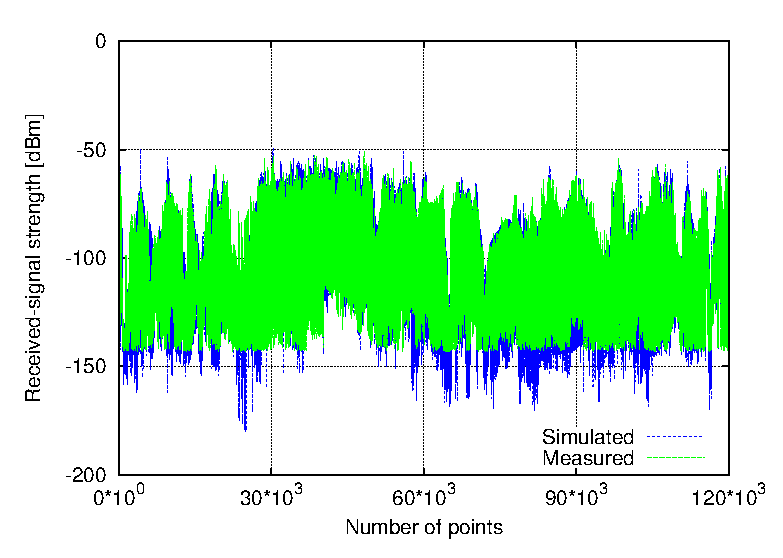
\includegraphics[width=0.47\textwidth]{08-real_network_planning/img/lte_prato_rcv_pwr}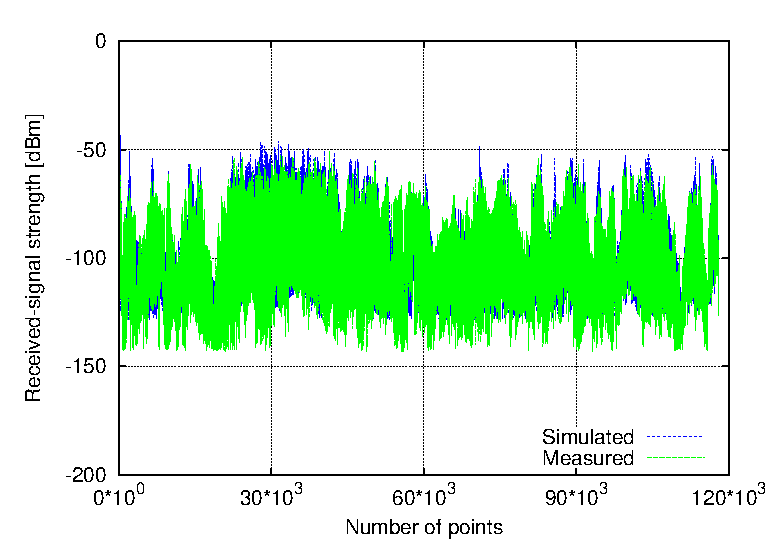
\includegraphics[width=0.47\textwidth]{08-real_network_planning/img/lte_tcpu_rcv_pwr}\\\hspace{0.4cm}(a)\hspace{6.7cm}(b)

\caption{Net$_{13}$ distribution of the predicted received-signal powers (LTE)
compared to field measurements for: (a) PRATO, and (b) the commercial
radio-planning tool.\label{fig:08-Received_signal_power-LTE}}
\end{figure}


Figure~\ref{fig:08-Received_signal_power-GSM}~(a), that depicts
the received-power levels for Net$_{11}$ (GSM), shows that the prediction
results match the field measurements rather well. A similar result
arrangement can be observed in Figure~\ref{fig:08-Received_signal_power-UMTS}~(a)
for Net$_{12}$ (UMTS), whereas the prediction results for Net$_{13}$
(LTE) show a slightly increased deviation from the field measurements,
as presented in Figure~\ref{fig:08-Received_signal_power-LTE}~(a).

\begin{figure}[h]
\centering

\includegraphics[width=0.6\textwidth]{08-real_network_planning/img/gsm_diff}

\caption{Probability distribution function for Net$_{11}$ (GSM) of the difference
between the field measurements and the simulation results of PRATO,
and the commercial tool. \label{fig:08-Prediction_difference-GSM}}
\end{figure}


\begin{figure}[h]
\centering

\includegraphics[width=0.6\textwidth]{08-real_network_planning/img/umts_diff}

\caption{Probability distribution function for Net$_{12}$ (UMTS) of the difference
between the field measurements and the simulation results of PRATO,
and the commercial tool.\label{fig:08-Prediction_difference-UMTS}}
\end{figure}


\begin{figure}[h]
\centering

\includegraphics[width=0.6\textwidth]{08-real_network_planning/img/lte_diff}

\caption{Probability distribution function for Net$_{13}$ (LTE) of the difference
between the field measurements and the simulation results of PRATO,
and the commercial tool.\label{fig:08-Prediction_difference-LTE}}
\end{figure}


Plots showing the probability distribution function (PDF\nomenclature[A]{PDF}{Probability distribution function})
of the difference between the simulation results and the field measurements
were also produced. In this case, Figures~\ref{fig:08-Prediction_difference-GSM},
\ref{fig:08-Prediction_difference-UMTS}, and~\ref{fig:08-Prediction_difference-LTE}
show graphs representing the difference, expressed in dB, between
the predictions and measurements of Net$_{11}$, Net$_{12}$ and Net$_{13}$,
respectively. Again, the graphs labeled as (a) show the analysis for
PRATO, whereas the ones labeled as (b) show the same analysis for
the commercial tool. Table~\ref{tab:08-PDF_properties} lists the
mean and standard deviation of the PDFs for each network and tool
tested, the values of which are expressed in dB. It is important to
note that the parameter set used for both tools intentionally generate
pessimistic results in terms of coverage prediction. This is clearly
observed from the mean-difference values of all three test cases.

\begin{table}
\centering

\caption{Mean and standard-deviation values for the PDFs of the difference
between simulation and measurement results.\textit{\emph{ }}\textit{\label{tab:08-PDF_properties}}}


\begin{tabular}{cccccc}
\cmidrule{2-6} 
 & \multicolumn{2}{c}{Mean {[}dB{]}} &  & \multicolumn{2}{c}{Std. deviation {[}dB{]}}\tabularnewline\addlinespace
\cmidrule{2-6} 
 & PRATO & Commercial tool &  & PRATO & Commercial tool\tabularnewline\addlinespace
\midrule
Net$_{11}$ & 9.37 & 12.04 &  & 12.29 & 11.98\tabularnewline
Net$_{12}$ & 9.31 & 8.71 &  & 11.94 & 11.23\tabularnewline
Net$_{13}$ & 3.84 & 3.63 &  & 12.20 & 11.06\tabularnewline
\bottomrule
\end{tabular}
\end{table}


Comparing the plots for each of the test networks (see Figures~\ref{fig:08-Prediction_difference-GSM},
\ref{fig:08-Prediction_difference-UMTS}, and~\ref{fig:08-Prediction_difference-LTE}),
it is clear that the difference between each pair of (a) and (b) diagrams
is minor. A small difference is present on the commercial tool, the
predictions of which show a slightly greater deviation with respect
to the measurements. Therefore, it can be concluded that the prediction
results of PRATO are comparable with the results of the commercial
tool for the three test networks. Moreover, the presented analysis
also confirms that the calculated results are independent of the frequency
band used, since each test network operates in a different frequency.

Additionally, each of the test networks extended over different terrain
types and environments, e.g., urban and suburban areas. Since the
curves of the presented charts show similar profiles for the difference
between the measurements and simulations for both tools, the applicability
of PRATO for arbitrary terrain types can also be expected.

Notice also that PRATO generated similar results as the commercial
tool in all three cases, irrespective of the operational frequency
or chosen terrain type. The predicted values are also comparable for
different distances between the BSs and UEs. Moreover, a slight improvement
can be observed in some of the prediction values of PRATO, because
they better resemble the profile shown by the field measurements.


\subsection*{Computational-time performance}

In the following, the computational-time performance of both tools
is analyzed. The analysis focused on the required processing times
of both tools on the same system, the hardware of which consisted
of a 4-core Intel i7 2.67~GHz CPU, 24~GB of RAM and a dual nVidia
GeForce GTX 590 GPU. The simulations for PRATO were performed on a
Linux operating system, using multiple processes on the CPU. The commercial
tool required a Windows Server operating system, and provided single-process,
multi-threading support to use all the cores of the CPU.

The simulations included the test networks presented above, all of
which extend over a geographical region of 285~x~185~km$^{2}$,
with a resolution of 25~m. The processing times for a set of simulations
are given in Figures~\ref{fig:08-Running_times-GSM}, \ref{fig:08-Running_times-UMTS},
and~\ref{fig:08-Running_times-LTE}, for test networks Net$_{11}$,
Net$_{12}$ and Net$_{13}$, respectively.

\begin{figure}[h]
\centering

\includegraphics[width=0.7\textwidth]{08-real_network_planning/img/gsm_running_times}

\caption{Simulation-processing times and speedup factors of Net$_{11}$ (GSM)
for the commercial tool and two implementations of PRATO. \label{fig:08-Running_times-GSM}}
\end{figure}


\begin{figure}[h]
\centering

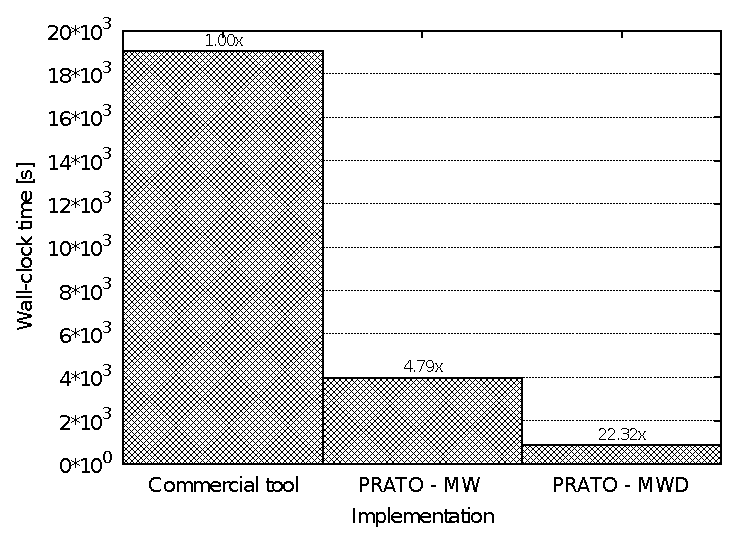
\includegraphics[width=0.7\textwidth]{08-real_network_planning/img/umts_running_times}

\caption{Simulation-processing times and speedup factors of Net$_{12}$ (UMTS)
for the commercial tool and two implementations of PRATO. \label{fig:08-Running_times-UMTS}}
\end{figure}


\begin{figure}[h]
\centering

\includegraphics[width=0.7\textwidth]{08-real_network_planning/img/lte_running_times}

\caption{Simulation-processing times and speedup factors of Net$_{13}$ (LTE)
for the commercial tool and two implementations of PRATO. \label{fig:08-Running_times-LTE}}
\end{figure}


The plotted values represent the average simulation-processing time
after performing 10 independent measurements. The time-measurement
gathering was performed during the simulations presented in the previous
section. The PRATO-CPU deployed used six workers and one master process.
For the PRATO-GPU configuration, the same process deployment was used,
and the worker processes operated on the dual GPU, i.e., two GPUs
on one board, each of which featured 1.5~GB of DRAM. 

The benefits of the parallel implementation of PRATO is clear in all
three cases. Moreover, the multi-GPU support increases the running-time
performance even further, achieving speedup factors of 18.96, 22.32,
and 9.95, for Net$_{11}$, Net$_{12}$, and Net$_{13}$, respectively.
These results confirm that the use PRATO as a radio-planning tool
in a real-world environment is feasible and it outperforms the compared
commercial tool in terms of computational-time performance.


\section{Summary}

The radio planning of modern cellular networks requires efficient
and exact radio-signal coverage calculations. In this context, the
unified framework PRATO was evaluated from a radio-network planning
point-of-view by comparing its simulation results with field measurements.
The same analysis was applied to a professional software application
in order to assess the results of PRATO from a quality and performance
perspectives.

The extensive analyses presented in this chapter showed satisfactory
results. Compared to a professional network-planning tool, the result
accuracy achieved is completely comparable irrespective of the terrain
type or operational frequency, while the computational speed is many
times higher. These results confirm that PRATO does not reduce the
solution quality due to the increased performance. Indeed, its suitability
for use in a real-world environment, addressing different radio-planning
activities by simulation, was also confirmed. This fact makes the
framework interesting for researchers as well as for radio-network
engineers.
\cleardoublepage{}


\chapter{Conclusion and further work}

\noindent First paragraph in current heading. First paragraph in current
heading. First paragraph in current heading. First paragraph in current
heading. First paragraph in current heading. First paragraph in current
heading. First paragraph in current heading. First paragraph in current
heading. First paragraph in current heading.

Next paragraph in current heading. Next paragraph in current heading.
Next paragraph in current heading. Next paragraph in current heading.
Next paragraph in current heading. Next paragraph in current heading.
Next paragraph in current heading. Next paragraph in current heading.
Next paragraph in current heading.

Next paragraph in current heading. Next paragraph in current heading.
Next paragraph in current heading. Next paragraph in current heading.
Next paragraph in current heading. Next paragraph in current heading.
Next paragraph in current heading. Next paragraph in current heading.
Next paragraph in current heading.
 \cleardoublepage{}


\chapter{Acknowledgments}

% First paragraph has no indentation.

\noindent The authors would like to especially thank the radio engineers
at Telekom Slovenije, d.d., for cooperating and sharing their professional
expertise throughout the creation of this work. This project was co-financed
by the European Union, through the European Social Fund.

The contents presented in Chapter~\ref{chap:04-Framework-design-and-implementation}
are the results of joint research work, conducted with the Nagasaki
Advanced Computer Center (NACC) of the Nagasaki University. In this
context, T. Hamada, head of NACC, acknowledges support from the Japan
Society for the Promotion of Science (JSPS) through its Funding Program
for World-leading Innovative R\&D on Science and Technology (First
Program).

The authors would like to especially thank the staff at the Nagasaki
Advanced Computing Center (NACC) of the Nagasaki University for their
support while making the computer cluster DEGIMA available for the
experimental simulations. We are also grateful with the radio engineers
at Telekom Slovenije, d.d., for supplying the network data sets and
sharing their professional expertise throughout the creation of this
work.

This project was co-financed by the European Union, through the European
Social Fund.
 \cleardoublepage{}

%\thispagestyle{plain}

\bibliographystyle{nature}
\bibliography{01-introduction/01-introduction,02-background_and_motivation/02-background_and_motivation,04-framework_design_and_implementation/04-framework_design_and_implementation,05-framework_parameter_tuning/05-framework_parameter_tuning,07-experimental_evaluation/07-01-soft_handover_alignment,07-experimental_evaluation/07-02-service_coverage_problem}


\cleardoublepage{} \listoffigures


\cleardoublepage{} \listoftables


\cleardoublepage{}\addcontentsline{toc}{chapter}{Index of Algorithms} 

\listof{myalgorithm}{Index of Algorithms} 

\appendix
%dummy comment inserted by tex2lyx to ensure that this paragraph is not empty
%%
%To not show sections in TOC use new command \tocless (uncomment next two lines)
%\newcommand{\nocontentsline}[3]{}
%\newcommand{\tocless}[2]{\bgroup\let\addcontentsline=\nocontentsline#1{#2}\egroup}
%% Example:
%\tocless\section{hide}
%\tocless\subsection{subhide}
%%


\renewcommand*{\thechapter}{ } \renewcommand*{\thesection}{\Alph{section}}
\chapter{Appendix}
\section{Appendix 1}
\noindent
List of publications related to this dissertation.
 \cleardoublepage{}

\section{Appendix 2}
\noindent
This is another appendix.

\end{document}
